\clearpage

\chapter{A SICStus \clpfd könyvtára}

A következő fejezetben a SICStus \clpfd könyvtárával fogunk foglalkozni.
A \clpfd könyvtárat az alábbi módon lehet használatba venni:
\begin{verbatim}
:- use_module(library(clpfd)).
\end{verbatim}

\section{A \clpfd könyvtár általános jellemzése}

A \clpfd könyvtár az egész számok véges tartományain (\emph{finite domain, FD})
alapuló CLP rendszert valósít meg. A könyvtár általános alapelve, hogy a
CLP relációkat a \cd{\#} jellel kell kezdeni, ezzel különböztetve meg őket
a hagyományos Prolog jelektől.

\enum{Felhasználható függvények}{
\item kétargumentumúak: {\tt +, -, *, /, mod, min, max}
\item egyargumentumú: {\tt abs} \\
Ezek a hagyományos matematikai műveletekkel megegyező funkcióval rendelkeznek.
}
\enum{Felhasználható relációk}{
\item aritmetikaiak: \cd{\#<, \#>, \#=<, \#>=, \#= \#\bs=}\\
Ezek a jól ismert Prolog relációjelek megfelelői, mindegyik \cd{xfx 700}
típusú operátor.
\item halmazműveletek:
\begin{itemize}
  \item \cd{\var{X} in \var{Halmaz}} ---
     \cd{\var{X}} értékét \cd{\var{Halmaz}}-ból veszi
  \item \cd{domain([\var{Változók},\ldots], \var{Min}, \var{Max})} ---
     \cd{\var{Változók}} minden változója értékét a
     \cd{\var{Min}}..\cd{\var{Max}} intervallumból veszi
\end{itemize}
ahol \cd{\var{Halmaz}} lehet:
\begin{itemize}
\item felsorolás: \cd{\{\var{Szám},\ldots\}}
\item intervallum: \cd{\var{Min}..\var{Max}} (\cd{xfx 550} operátor)
\item két halmaz metszete: \cd{\var{Halmaz} \cd{/\bs} \var{Halmaz}}
    (\cd{yfx 500} beépített operátor)
\item két halmaz uniója: \cd{\var{Halmaz} \cd{\bs/} \var{Halmaz}}
    (\cd{yfx 500} beépített operátor)
\item egy másik halmaz komplemense: \cd{\bs\var{Halmaz}}
    (\cd{fy 500} operátor)
\end{itemize}
}

\cd{\var{Min}}-re megengedett az \cd{inf} névkonstans, ami az alsó korlát
hiányát jelenti ($-\infty$), hasonlóan \cd{\var{Max}}-ra megengedett a \cd{sup}
névkonstans, ami pedig a felső korlát hiányát jelenti ($+\infty$). A végtelen
korlátok általában csak kényelmi célokat használnak abban az esetben, ha
a tényleges korlátok kikövetkeztethetőek. Effektíven végtelen korlátokkal
rendelkező változóknak nem sok értelmük van, mert azok a címkézés (ld. később)
során végtelen választási pontot hoznának létre (éppen ezért nem lehet olyan
változókat címkézni, amelyek végtelen tartománnyal rendelkeznek).
\br
A \clpfd világban egyszerű korlátoknak csak az \cd{\var{X} $\in$ \var{Halmaz}}
jellegű korlátokat tekintjük, minden más összetett korlátnak számít, éppen
ezért nagyon nagy hangsúly van az összetett korlátok erősítő tevékenységén
(ellentétben a \Clpb -vel, ahol nem is voltak összetett korlátok). Ez a tény
(illetve a \clpfd ,,lustasága'') teszi lehetővé azt, hogy nagyobb problémákat
is megoldjunk vele. Az összetett korlátok erősítő tevékenysége a mesterséges
intelligencia-kutatások CSP (Constraint Satisfactory Problems) ágának
módszerein alapul.

Egy egyszerű \clpfd példa:

\begin{verbatim}
| ?- X in (10..20)/\ (\{15}), Y in 6..sup, Z #= X+Y.
X in(10..14)\/(16..20), Y in 6..sup, Z in 16..sup ?
\end{verbatim}
\begin{verbatim}
| ?- X in 10..20, X #\= 15, Y in {2}, Z #= X*Y.
   Y = 2, X in(10..14)\/(16..20), Z in 20..40 ?
\end{verbatim}

A második példán lustaságon kaphatjuk rajta a \clpfd következtető mechanizmust:
ugyan kikövetkeztethető lenne, hogy \cd{Z} csak 20 és 40 közötti \emph{páros}
szám lehet (mivel \cd{Y} páros, és \cd{X} 10 és 20 között van), sőt még
az is, hogy \cd{Z} semmiképp nem lehet 30 (mert \cd{X} sem lehet 15),
de ezt a \clpfd nem teszi meg, helyette egyszerűen megnézi \cd{X} alsó és
felső határát (10 és 20), ezeket beszorozza \cd{Y} alsó és felső határával
(ez jelen esetben azonos: 2 és 2), majd az így kapott négy szám minimuma és
maximuma által megadott intervallumra szűkíti \cd{Z}-t. Ezt a mechanizmust
\emph{intervallum-szűkítés}nek nevezzük, és az \ref{szukites} fejezetben
részletesen foglalkozunk majd vele.

\section{A \clpfd feladatok megoldási struktúrája}

Minden \clpfd feladat megoldása hasonló struktúrájú programot eredményez,
ezért érdemes megkülönböztetnünk a megoldási folyamat fő lépéseit:

\begin{enumerate}
\item {\bf A probléma leképezése a \clpfd világra} \\
    Ebben a lépésben a problémának egy olyan modelljét kell megalkotnunk,
    amelyben a probléma egyes elemeit \clpfd fogalmakra (változókra,
    értéktartományokra) képezzük le.

\item {\bf Változók és korlátok felvétele} \\
    Ebben a lépésben be kell vezetnünk a feladatban szereplő változókat,
    és fel kell vennünk a változók között fennálló korlát-relációkat.

\item {\bf Címkézés} \\
    Ha a problémának a korlátok alapján nincs egyértelmű megoldása, vagy
    ezt a rendszer nem tudta kikövetkeztetni, akkor a változókat el kell
    kezdenünk szisztematikusan az értéktartományaik egy-egy lehetséges
    értékéhez kötni, így meg fogjuk kapni a probléma összes megoldását.
    A címkézési folyamat a \clpb könyvtárnál látotthoz hasonló módon
    működik, de itt egy változó nem csak kétfajta értéket vehet fel.
    Ha a problémának a korlátok felvétele után már egyértelmű a megoldása,
    akkor a címkézési fázis elmarad.
\end{enumerate}

Lássuk a fent elmondottakat egy konkrét példán! A feladat az alábbi térkép
kiszínezése kék, piros és sárga színekkel úgy, hogy a szomszédos országok
különböző színűek legyenek, és ha két ország határán a \cd{<} jel van, akkor
a két szín ábécé-rendben a megadott módon kövesse egymást.

\begin{center}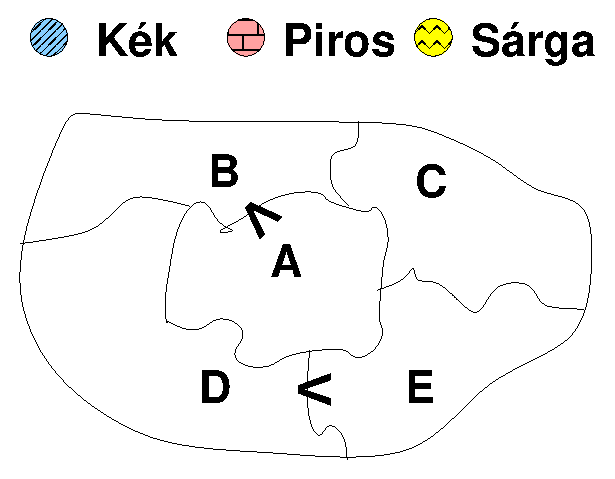
\epsfig{file=terkep.eps,width=0.2\textwidth}\end{center}

Egy lehetséges megoldási folyamat (\emph{zárójelben a CSP elnevezések}):

\begin{enumerate}
\item Minden mezőben elhelyezzük a három lehetséges színt ({\em változók és
tartományaik felvétele}).
\item Az ,,A'' mező nem lehet kék, mert annál ,,B'' nem lehetne kisebb.
A ,,B'' nem lehet sárga, mert annál ,,A'' nem lehetne nagyobb. Az ,,E'' és
,,D'' mezők hasonlóan szűkíthetők ({\em szűkítés, él-konzisztencia biztosítása}).
\item Ha az ,,A'' mező piros lenne, akkor mind ,,B'', mind ,,D'' kék lenne,
ami ellentmondás ({\em globális korlát, ill.\ borotválási technika}).
Tehát ,,A'' sárga. Emiatt a vele szomszédos ,,C'' és ,,E'' nem lehet sárga
({\em él-konszitens szűkítés}).
\item ,,C'' és ,,D'' nem lehet piros, tehát kék, így ,,B'' csak piros
lehet ({\em él-konszitens szűkítés}). Tehát az egyetlen megoldás:\\
A~=~sárga, B~=~piros, C~=~kék, D~=~kék, E~=~piros.
\end{enumerate}

Az alábbi ábrasorozaton láthatóak az egyes lépésekhez tartozó állapotok:

\btab{cccc}
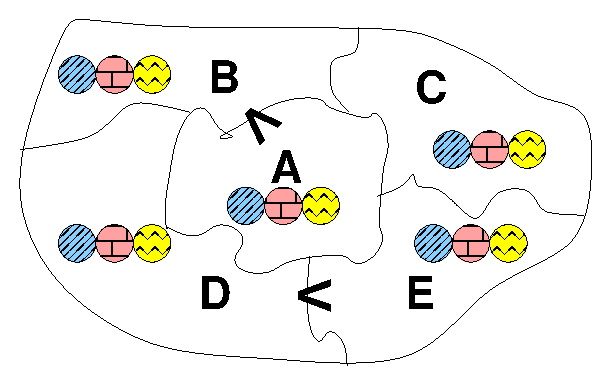
\epsfig{file=terkep2.eps,width=0.18\textwidth} &
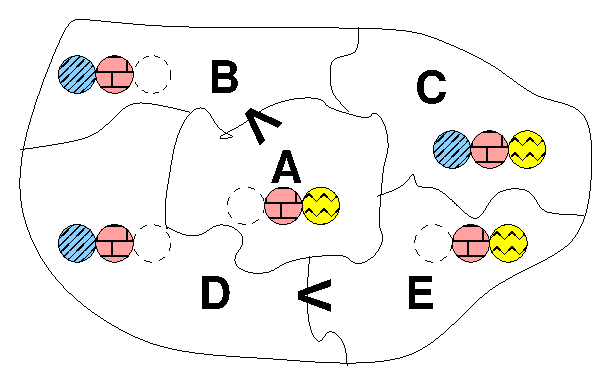
\epsfig{file=terkep3.eps,width=0.18\textwidth} &
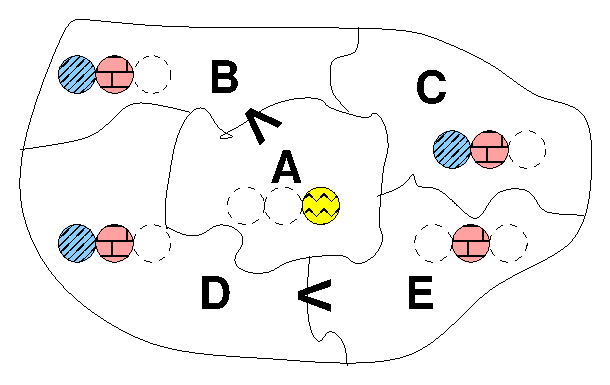
\epsfig{file=terkep4.eps,width=0.18\textwidth} &
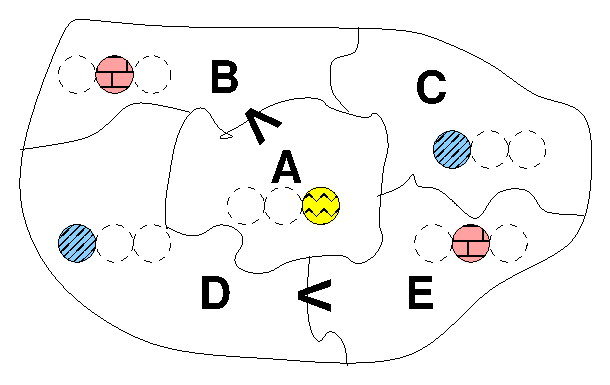
\epsfig{file=terkep5.eps,width=0.18\textwidth} \\
1. lépés & 2. lépés & 3. lépés & 4. lépés
\etab

\section{A CSP problémakör áttekintése}
\label{cspfogalmak}

Mint említettük, a \clpfd könyvtár a mesterséges intelligencia CSP megoldási
módszerein alapul, ezért mielőtt továbbmennénk, érdemes áttekinteni a CSP
problémakör fogalmait és eredményeit.

\enum{A CSP fogalma}{
\item Egy CSP-t egy $(X,D,C)$ hármassal jellemezhetünk, ahol
  \begin{itemize}
  \item $X = \tuple{x_1,\dots,x_n}$~--- változók
  \item $D = \tuple{D_1,\dots,D_n}$~--- tartományok, azaz nem üres halmazok
  \item $x_i$ változó a $D_i$ véges halmazból ($x_i$ tartománya) vehet fel
  értéket ($\forall i$-re $x_i \in D_i$)
  \item $C$ a problémában szereplő korlátok (atomi relációk) halmaza,
  argumentumaik $X$ változói (például $C \ni c = r(x_1,x_3)$, $r \subseteq D_1 \times
  D_3$)
  \end{itemize}
\item A CSP feladat megoldása: minden $x_i$ változóhoz egy  $v_i\in D_i$
  értéket kell rendelni úgy, hogy minden $c\in C$ korlátot egyidejűleg
  kielégítsünk.
}

\definicio egy $c$ korlát egy $x_i$ változójának $d_i$ értéke
  \emph{felesleges}, ha nincs a $c$ többi változójának olyan értékrendszere,
  amely $x_i=d_i$-vel együtt kielégíti $c$-t.
\br
\tetel felesleges érték elhagyásával (szűkítés) ekvivalens CSP-t kapunk.
\br
\definicio egy korlát \emph{élkonzisztens} (\emph{arc consistent}),
  ha egyik változójának tartományában sincs felesleges érték. A CSP
  \emph{élkonzisztens}, ha minden korlátja élkonzisztens. Az élkonzisztencia
  szűkítéssel biztosítható.
\br
Az \emph{élkonzisztencia} elnevezés onnan ered, hogy ha minden reláció
bináris, akkor a CSP probléma egy gráffal ábrázolható, ahol minden változónak
egy csomópont, minden relációnak egy él felel meg.

\enum{A CSP megoldás folyamata}{
\item felvesszük a változók tartományait;
\item felvesszük a korlátokat mint démonokat, amelyek szűkítéssel
él-konzisztenciát biztosítanak;
\item többértelműség esetén címkézést (labeling) végzünk:
\begin{itemize}
\item kiválasztunk egy változót (pl.a legkisebb tartományút),
\item a tartományt két vagy több részre osztjuk (választási pont),
\item az egyes választásokat visszalépéses kereséssel bejárjuk
(egy tartomány üresre szűkülése váltja ki a visszalépést).
\end{itemize}
}

A térképszínezés, mint CSP feladat esetén minden országhoz egy változót
rendeltünk hozzá, ennek a változónak az értéke fogja az ország színét
kódolni. A színekhez ábécésorrend szerint az 1, 2, 3 értékek valamelyikét
rendeltük hozzá (kék $\to$ 1, piros $\to$ 2, sárga $\to$ 3), majd felvettük a
korlátokat egyrészt arra, hogy a szomszédos országok színei különböznek (ez a
változóértékek világában egy $\neq$ típusú relációt jelent), másrészt arra, hogy
az országok színei között megadott < relációk is teljesüljenek. Ezzel
kaptunk egy kiinduló korlát-gráfot, amit a felesleges élek elhagyásával
szűkítettünk. Az alábbi ábrán látható a kiinduló korlát-gráf és annak
élkonzisztens szűkített változata:

\btab{cp{5em}c}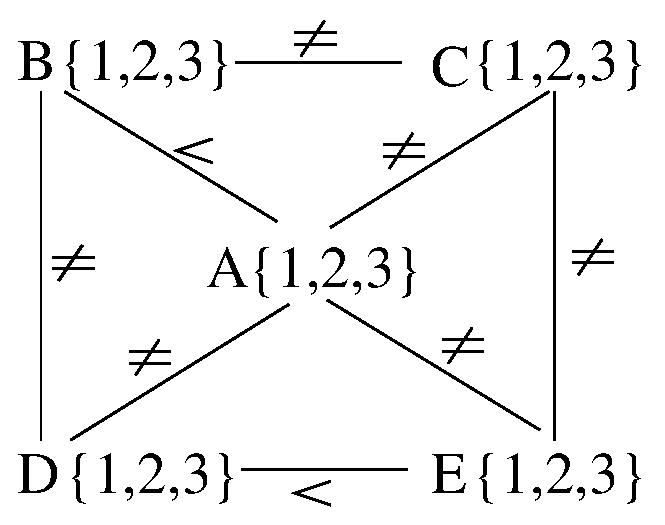
\epsfig{file=korlatok.eps,width=0.25\textwidth} & &
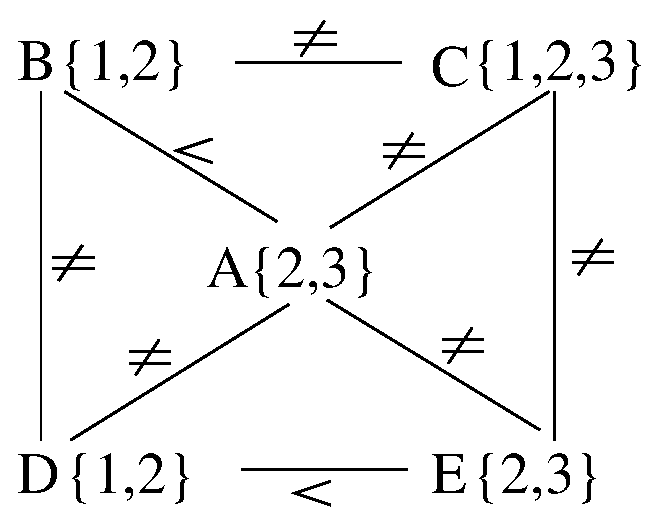
\epsfig{file=korlatok_elk.eps,width=0.25\textwidth}\etab

A CSP sémának a CLP világba történő beágyazásával kapjuk a SICStusban lévő
\clpfd könyvtárat. Minden CSP változónak egy \clpfd változó feleltethető meg,
a CSP változók értéktartományainak pedig egy-egy \clpfd egyszerű korlát.
A többi CSP korlát összetett \clpfd korlátként jelenik meg. A \clpfd korlát-tár
új változótartomány felvételén vagy egy meglévő változó tartományának
szűkítésén módosulhat. Az összetett korlátok \emph{démon}ok lesznek, amelyek
hatásukat az \emph{erősítés}en keresztül fejtik ki (ld. \ref{erosit} fejezet).
Az erősítés mindig egyszerű korlátokat ad a korlát-tárhoz. A démonok ciklikusan
működnek: megszületnek, szűkítenek, elalszanak, aktiválódnak, szűkítenek,
elalszanak, \ldots aktiválódnak, szűkítenek, és amikor már levezethetőek a
korlát-tár tartalmából, akkor megszűnnek létezni. A démonokat mindig az
érintett korlátbeli változók tartományának módosulása aktiválja. A szűkítés
mértéke a démontól függ, néha nem előnyös az összes lehetséges szűkítést
elvégezni, mert túlságosan költséges lenne.

\section{A \clpfd könyvtár jellegzetességei}

Ebben az alfejezetben a \clpfd könyvtár néhány jellegzetességét mutatjuk be
példákon keresztül. A példák megértéséhez egyetlen, nagyon fontos állítást
kell szem előtt tartanunk: {\bf a \clpfd démonok csak a korlát-táron keresztül
hatnak egymásra!}
\br
A fenti mondat azt takarja, hogy a démonok nem ,,látják'' egymást, az
egymással való interakciójukat kizárólag a korlát-táron keresztül
végzik: az egyik démon szűkíti a korlát-tárat, ennek hatására egy
másik démon felébred, szűkít, erre egy harmadik démon ébred fel
és így tovább... Előfordulhatnak azonban olyan esetek, amikor egyik
démon sem tud felébredni, és így esetleg egy nyilvánvaló ellentmondást
nem vesz észre a rendszer, mint például a következő példában:

\begin{verbatim}
| ?- domain([X,Y,Z], 1, 2), X #\= Y, X #\= Z, Y #\= Z.
X in 1..2,
Y in 1..2,
Z in 1..2 ? ;
no
\end{verbatim}

Mivel \cd{X}, \cd{Y} és \cd{Z} értékkészlete is az 1 és a 2 számokból
áll, és az \cd{X \#\bs= Y} jellegű korlátok démonai csak akkor ébrednek fel, ha
valamelyik változójuk behelyettesített lesz, ezért egyik démon sem tud szűkíteni,
és az ellentmondás nem derül ki. A megoldást globális korlátok (pl. az
\cd{all_distinct/1}) használata jelenti majd. A globális korlátok olyan korlátok,
amelyek működésükkel több korlát hatását fogják össze egyetlen démonban, így
ez a démon rá tud jönni az ilyen jellegű ellentmondásokra. Ezekről a korlátokról
a későbbiekben még részletesen lesz szó (ld. \ref{globalis}. fejezet).

Hasonló szituációt jelent a következő példa is:

\begin{verbatim}
| ?- X #> Y, Y #> X.
Y in inf..sup,
X in inf..sup ? ;
no
\end{verbatim}

Ha ugyanezt a két korlátot úgy vesszük fel, hogy közben \cd{X} és \cd{Y} tartományát
végesre szűkítjük, akkor már nem jelentkezik a probléma:

\begin{verbatim}
| ?- domain([X,Y], 1, 10), X #> Y, Y #> X.
no
\end{verbatim}

Azonban ha a tartományt egy picit tágabbra vesszük, újabb problémával találjuk
szembe magunkat, a meglepően nagy futási idővel:

\begin{verbatim}
| ?- statistics(runtime,_),
     ( domain([X,Y], 1, 100000), X #> Y, Y #> X
     ; statistics(runtime,[_,T])
     ).
T = 3630 ? ;
no
\end{verbatim}

Ennek oka ismét abban keresendő, hogy a démonok csak a korlát-táron keresztül
hatnak egymásra. Nézzük meg ugyanis ennek a példának a futását az \fdbg
nyomkövető könyvtár használatával, 10-es tartományhatárra (az \fdbg könyvtárról
bővebben a \ref{fdbg}. fejezetben lesz szó)!

\begin{verbatim}
| ?- use_module(library(fdbg)).
| ?- fdbg_on, fdbg_assign_name(X, x), fdbg_assign_name(Y, y),
     domain([X,Y], 1, 10), X #> Y, Y #> X.

domain([<x>,<y>], ==> x = inf..sup -> 1..10,
       1,10)          y = inf..sup -> 1..10
                      Constraint exited.

<x> #>= <y>+1     ==> x = 1..10 -> 2..10,   y = 1..10 -> 1..9

<x>+1 #=< <y>     ==> x = 2..10 -> 2..8,    y = 1..9 -> 3..9

<x> #>= <y>+1     ==> x = 2..8 -> 4..8,     y = 3..9 -> 3..7

<x>+1 #=< <y>     ==> x = 4..8 -> 4..6,     y = 3..7 -> 5..7

<x> #>= <y>+1     ==> x = 4..6 -> {6},      y = 5..7 -> {5}
                      Constraint exited.

2 #=< 0           ==> Constraint failed.
% Valójában a korlát <x>+1 #=< <y>, azaz 6+1 #=< 5
no
\end{verbatim}

A kimenetet értelmezve láthatjuk, hogy az \cd{X} és az \cd{Y} változók
tartománya nagyon lassan szűkül: kezdetben az \cd{X in 1..10} feltétel
és az \cd{X \#> Y} (a \clpfd belső ábrázolása szerint \cd{X \#>= Y+1})
korlát démona miatt \cd{X} tartománya a \cd{2..10} halmazra, \cd{Y}-é pedig
az \cd{1..9}-re szűkül. Ekkor a tartománymódosulások hatására felébred
az \cd{Y \#> X} korlát démona is, és szűkíti \cd{X}-et a \cd{2..8}, \cd{Y}-t
a \cd{3..9} halmazra. Ettől viszont újból felébred az \cd{X \#> Y} korlát
démona, és így folytatódik a dolog egészen addig, amíg végül az egyik
démon észre nem veszi, hogy itt meghiúsulás fog következni. Nagyobb
tartományhatárok esetén ez a láncreakció értelemszerűen tovább tart, sőt,
mint láttuk, végtelen tartományhatárok esetén nem is indul el.

\section{Egyszerű constraint feladatok megoldása}

\subsection{Térképszínezés}

Emlékeztetőül a feladat: színezzük ki az alábbi térképet kék, piros és
sárga színekkel úgy, hogy a szomszédos országok különböző színűek legyenek,
és ha két ország határán a \cd{<} jel van, akkor a két szín ábécé-rendben
a megadott módon kövesse egymást.

\begin{center}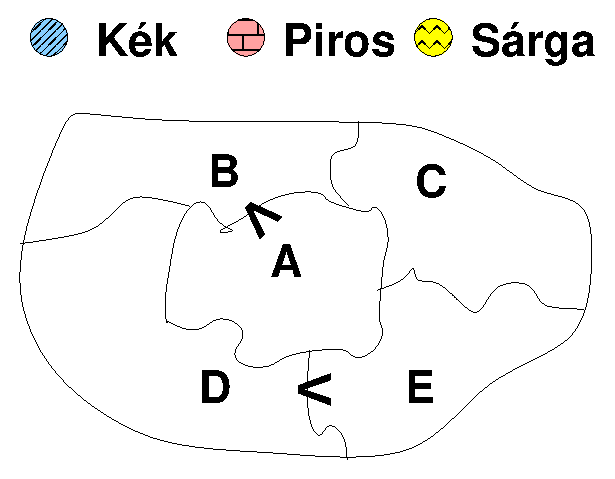
\epsfig{file=terkep.eps,width=0.2\textwidth}\end{center}

Először írjuk fel a megfelelő korlátokat leíró \clpfd célsorozatot:

\begin{alltt}
| ?- use_module(library(clpfd)).
...
| ?- domain([A,B,C,D,E], 1, 3),
     A #> B, A #\bs= C, A #\bs= D, A #\bs= E,
     B #\bs= C, B #\bs= D, C #\bs= E, D #< E.
A in 2..3, B in 1..2, C in 1..3, D in 1..2, E in 2..3 ? ;
no
\end{alltt}

Látható, hogy a Prolog az élkonzisztencia biztosítását elvégezte, de a
megoldást még nem tudta kikövetkeztetni. A megoldások meghatározásához
meg kell kérni a rendszert, hogy az \cd{A} változót rendre helyettesítse
be az 1, 2, 3 értékekre. Ez többféleképpen is elvégezhető: egyrészt a
hagyományos \cd{member/2} eljárással, amelynél azonban egyesével fel kell
sorolnunk \cd{A} lehetséges értékeit, ami nagy értékkészletnél kényelmetlen
lehet:

\begin{alltt}
| ?- domain([A,B,C,D,E], 1, 3),
     A #> B, A #\bs= C, A #\bs= D, A #\bs= E,
     B #\bs= C, B #\bs= D, C #\bs= E, D #< E,
     member(A, [1,2,3]).
A = 3, B = 2, C = 1, D = 1, E = 2 ?
\end{alltt}

Az ilyen problémák megoldására szolgál az \cd{indomain/1} eljárás, amely
ezt a behelyettesítést automatikusan elvégzi a paraméterként adott változóra:

\begin{alltt}
| ?- domain([A,B,C,D,E], 1, 3), \ldots, indomain(A).
A = 3, B = 2, C = 1, D = 1, E = 2 ?
\end{alltt}

Előfordulhatott volna azonban, hogy \cd{A} behelyettesítése még mindig
nem elég ahhoz, hogy kiderüljön az összes megoldás, ezért célszerű
a behelyettesítést mind az 5 változóra elvégezni. Ezt a \cd{labeling/2}
eljárás végzi, amely első paramétere egy opciólista, amely a címkézés
menetét szabályozza (ezzel majd később foglalkozunk), második paramétere
pedig egy változólista, amelyre a címkézést el akarjuk végezni.

\begin{alltt}
| ?- domain([A,B,C,D,E], 1, 3), \ldots, labeling([],[A,B,C,D,E]).
A = 3, B = 2, C = 1, D = 1, E = 2 ?
\end{alltt}

Annak megfogalmazására, hogy az \cd{A}, \cd{C} és \cd{E} változók értéke
mind különbözik, a Prolog kínál egy egyszerűbb és hatékonyabb megoldást is,
az \cd{all_distinct/1} predikátumot. Ez egy listát vár paraméterként, és
ügyel arra, hogy a lista összes eleme különböző értékeket vegyen fel.

\begin{alltt}
| ?- domain([A,B,C,D,E], 1, 3),
     A #> B, A #\bs= E, B #\bs= C, B #\bs= D, D #< E,
     all_distinct([A,C,E]).
A = 3, B = 2, C = 1, D = 1, E = 2 ? ; no
\end{alltt}

Látható, hogy itt már címkézésre se volt szükség, mivel az \cd{all_distinct}
korlát ,,erősebb'' a páronkénti különbözőségnél.

\subsection{Kódaritmetika (SEND+MORE=MONEY)}

\label{sendmoremoney}

A feladvány: írjon a betűk helyébe tízes számrendszerbeli számjegyeket
(azonosak helyébe azonosakat, különbözőek helyébe különbözőeket) úgy, hogy a
SEND+MORE=MONEY egyenlőség igaz legyen. Szám elején nem lehet 0 számjegy.

\begin{verbatim}
send(SEND, MORE, MONEY) :-
  length(List, 8),
  domain(List, 0, 9),               % tartományok
  send(List, SEND, MORE, MONEY),    % korlátok
  labeling([], List).               % címkézés
\end{verbatim}
\begin{verbatim}
send(List, SEND, MORE, MONEY) :-
  List=[S,E,N,D,M,O,R,Y],
  alldiff(List), S #\= 0, M #\= 0,
  SEND #=  1000*S+100*E+10*N+D,
  MORE #= 1000*M+100*O+10*R+E,
  MONEY #= 10000*M+1000*O+100*N+10*E+Y,
  SEND+MORE #= MONEY.
\end{verbatim}
\begin{alltt}
% alldiff(L): L elemei mind különbözőek (buta megvalósítás).
% Lényegében azonos a beépített all_different/1 kombinatorikai globális korláttal.
alldiff([]).
alldiff([X|Xs]) :- outof(X, Xs), alldiff(Xs).
\end{alltt}
\begin{verbatim}
outof(_, []).
outof(X, [Y|Ys]) :- X #\= Y, outof(X, Ys).
\end{verbatim}

A fenti programon jól látszik a szokásos \clpfd struktúra (tartományok
felvétele, korlátok felvétele, címkézés). Az ,,azonos betűk azonos számokat,
különböző betűk különböző számokat jelentenek'' kitételt egy saját
\cd{alldiff/1} predikátummal valósítjuk meg, amely lényegében megegyezik
az \cd{all_different/1} beépített globális korláttal. Fontos megjegyezni,
hogy az \cd{all_different/1} és az \cd{all_distinct/1} korlátok \emph{nem}
ekvivalensek, az előbbi csak páronkénti különbözőséget valósít meg! Gyakran
azonban ez is elég, és az \cd{all_different} emellett gyorsabb futást biztosít,
tehát néha érdemes használni~\cite{DBLP:conf/aaai/Regin94}. Ezen magyarázat után lássuk a program futását:

\begin{verbatim}
| ?- send(SEND, MORE, MONEY).
MORE = 1085, SEND = 9567, MONEY = 10652 ? ;
no
\end{verbatim}

Nézzük meg azt is, hogy mit adna ki a program, ha elhagynánk a címkézést:

\begin{verbatim}
| ?- List=[S,E,N,D,M,O,R,Y], domain(List, 0, 9),
     send(List, SEND, MORE, MONEY).
        List = [9,E,N,D,1,0,R,Y],
        SEND in 9222..9866,
        MORE in 1022..1088,
        MONEY in 10244..10888,
        E in 2..8, N in 2..8, D in 2..8,
        R in 2..8, Y in 2..8 ? ; no
\end{verbatim}

Amint látható, a rendszer helyből rájött arra, hogy mivel az eredmény öt
számjegyből áll, a két összeadandó viszont csak négyből, ezért \cd{M}
csak 1 lehet. Ha viszont \cd{M} 1, akkor \cd{S}-nek 9-nek kell lennie,
különben nem keletkezhet átvitel, ilyenkor viszont \cd{O} csak nulla lehet.
A többi változó értéke csak a címkézés után derül ki.

\subsection{A zebra feladat}
Szintén egy \Clpfd -ben könnyen megfogható feladat: adott 5 különböző
nemzetiségű ember, 5 különböző színű ház, 5 különböző foglalkozás, 5
különböző állat és 5 különböző ital. Egy embernek pontosan egy
foglalkozása, nemzetisége, háza, kedvenc itala és állata van. A
feladat az, hogy az ismert kötöttségek alapján megmondjuk, hogy melyik
nemzetiségű ember kedvenc állata a zebra. Az embereket megsorszámozzuk
1-től 5-ig, majd minden egyes foglalkozáshoz, nemzetiséghez, házhoz,
italhoz és állathoz egy constraint változót rendelünk, amely értékét
az 1..5 halmazból veszi fel. Egy ilyen változó $i$ értéke azt jelenti,
hogy az általa reprezentált tulajdonság az $i$. számú emberhez
tartozik. A kötöttségeket ez alapján könnyen felírhatjuk, például az,
hogy a diplomata háza a sárga, egyszerűen a két megfelelő
constraint-változó egyenlővé tételével biztosítható.  A kötöttségek a
programból könnyen kideríthetők, itt nem soroljuk fel őket. Az
egyetlen figyelmet érdemlő feltétel annak a megvalósítása, hogy
valaki egy adott ház szomszédjában lakik. Ezt a \cd{nextto/2} predikátum
kezeli. A \cd{nextto/2} tulajdonképpen egy vagylagos szerkezet, amit a
Prolog választási pontokkal valósít meg - vagyis spekulatív módon veszi fel a
vagy-kapcsolatban szereplő korlátokat, és minden lehetőségre
megpróbálja megoldani az aktuális korlát rendszert. Ez nem a legszerencsésebb
megoldás, mivel sok választási pont esetén rengeteg időt igényelhet. A
vagylagos szerkezetekről a \clpfd esettanulmányokban (\pageref{diszjunkcio}.
oldal) még lesz szó. Adott esetben a

\begin{verbatim}
nextto(A,B):- abs(A-B) #= 1.
\end{verbatim}

megoldás sokkal szerencsésebb lenne, mivel ez nem generál választási
pontokat.

\begin{verbatim}
:- use_module(library(lists)).
:- use_module(library(clpfd)).

zebra(ZOwner, All):-
  All = [England,Spain,Japan,Norway,Italy,
         Green,Red,Yellow,Blue,White,
         Painter,Diplomat,Violinist,Doctor,Sculptor,
         Dog,Zebra,Fox,Snail,Horse,
         Juice,Water,Tea,Coffee,Milk],
  domain(All, 1, 5),
  alldiff([England,Spain,Japan,Norway,Italy]),
  alldiff([Green,Red,Yellow,Blue,White]),
  alldiff([Painter,Diplomat,Violinist,Doctor,Sculptor]),
  alldiff([Dog,Zebra,Fox,Snail,Horse]),
  alldiff([Juice,Water,Tea,Coffee,Milk]),
  England = Red,          Spain = Dog,
  Japan = Painter,        Italy = Tea,
  Norway = 1,             Green = Coffee,
  Green #= White+1,       Sculptor = Snail,
  Diplomat = Yellow,      Milk = 3,
  Violinist = Juice,      nextto(Norway, Blue),
  nextto(Fox, Doctor),    nextto(Horse, Diplomat),
  labeling([ff], All),
  nth(N, [England,Spain,Japan,Norway,Italy], Zebra),
  nth(N, [england,spain,japan,norway,italy], ZOwner).

nextto(A, B) :-  A #= B+1.
nextto(A, B) :-  A #= B-1.
\end{verbatim}

\subsection{N királynő a sakktáblán}

A feladat elhelyezni egy $n * n$-es sakktáblán $n$ királynőt úgy, hogy
egyik se üsse a másikat.
\br
A megoldás minden királynőt külön oszlopba tesz, majd mindegyikükhöz
egy változót rendel, ami a királynő oszlopbeli pozícióját adja meg. A
változók tartományának deklarálása után minden két királynő között
felállít egy constraint-et (\cd{no\_threat/3}), ami azt adja meg, hogy
a két királynő nem üti egymást. Ehhez meg kell adni a két királynő
oszlopainak távolságát, ami itt az \cd{I} paraméter. Ezek után a
program végrehajtja a címkézést first-fail heurisztikával. A first-fail
elv mindig a legkisebb értékkészlettel rendelkező változót helyettesíti
be először, abban reménykedve, hogy így hamarabb kiderülnek a hibás ágak.
A címkézési módokról később lesz szó.

\label{no:threat}

\begin{verbatim}
:- use_module(library(clpfd)).

% A Qs lista N királynő biztonságos elhelyezését
% mutatja egy N*N-es sakktáblán. Ha a lista
% i. eleme j, akkor az i. királynőt az i. sor j.
% oszlopába kell helyezni.
queens(N, Qs):-
  length(Qs, N), domain(Qs, 1, N),
  safe(Qs),
  labeling([ff],Qs).  % first-fail elv

% safe(Qs): A Qs lista a királynők biztonságos
% elhelyezését írja le.
safe([]).
safe([Q|Qs]):-
  no_attack(Qs, Q, 1),
  safe(Qs).

% no_attack(Qs, Q, I): A Qs lista által leírt
% királynők egyike sem támadja a Q oszlopban levő
% kiralynőt, feltéve hogy Q és Qs távolsága I.
no_attack([],_,_).
no_attack([X|Xs], Y, I):-
  no_threat(X, Y, I),
  J is I+1, no_attack(Xs, Y, J).

% Az X és Y oszlopokban  I sortávolságra levő
% királynők nem támadják egymást.
no_threat(X, Y, I) :-
  Y #= X, Y #= X-I, Y #= X+I.
\end{verbatim}



\section{Szűkítési szintek}
\label{szukites}

A könnyebb megértés érdekében először informálisan, egy egyszerű
kétargumentumú relációra fogjuk megfogalmazni az \emph{intervallum-szűkítés}
és a \emph{tartományszűkítés} fogalmát, utána pedig formalizáljuk a
leírtakat.
\br
Tekintsünk egy $r(X,Y)$ bináris relációt! Ekkor $r$ \emph{tartományszűkítése}
során $X$ tartományából elhagyjuk az összes olyan $x$ értéket, amelyhez nem
található $Y$ tartományában olyan $y$ érték, hogy $r(x,y)$ fennáll. Hasonlóan
szűkítjük $Y$ tartományát is. A folyamat eredménye az élkonzisztencia (lásd
a fogalom definícióját a \ref{cspfogalmak} fejezetben).
\emph{Intervallum-szűkítés} során viszont $X$ tartományából elhagyjuk annak
alsó vagy felső határát, ha ahhoz nem található olyan $y$ érték, amely $Y$
határai közé esik, és azzal az $r$ reláció fennáll. Hasonlóan szűkítjük
$Y$ tartományának határait is, és ezeket a lépéseket addig ismételjük,
amíg tudunk szűkíteni. Ez a módszer nem biztosít élkonzisztenciát, de
gyorsabban elvégezhető.
\br
Példa: legyen $x \in \{0,1,2,3,4,5\}$ és $y \in \{-1,1,3,4\}$, $r(x,y)$ pedig
az $x=|y|$ reláció. A tartományszűkítés $x$ értékkészletéből elhagyja
a 0, 2, 5 értékeket, hiszen semelyik $y$ érték abszolútértéke nem lehet
sem 0, sem 2, sem 5. Az intervallum-szűkítés viszont először csak a 0
és az 5 kizárásával próbálkozik. 0-t nem zárhatja ki, hiszen $y$ tartományának
szélső értékei közé (tehát -1 és 4 közé) esik a 0, és $0=|0|$. 5-öt
kizárhatja, mert sem a -5, sem az 5 nem esik $y$ szélső értékei közé,
de a 4-et már nem zárhatja ki, ezért $x$ csak a $\{0,1,2,3,4\}$ halmazra
szűkül.
\br
A fenti példán jól látszik az intervallum-szűkítés két gyengesége:

\begin{enumerate}
\item csak a tartomány szélső értékeit hajlandó elhagyni, ezért nem hagyja el
a \cd{2} értéket;
\item a másik változó tartományában nem veszi figyelembe a ,,lyukakat'', így
a példában \cd{Y} tartománya helyett annak \emph{lefedő intervallumát}, azaz
a \cd{-1..4} intervallumot tekinti, ezért nem hagyja el \cd{X}-ből
a \cd{0} értéket.
\end{enumerate}

Ugyanakkor az intervallum-szűkítés általában konstans idejű művelet,
míg a tartományszűkítés ideje (és az eredmény mérete) erősen függ a
tartományok méretétől, ezért sok esetben a SICStus \clpfd könyvtár csak
az intervallum-szűkítést garantálja, a tartományszűkítést nem.
\br
Ezek után fogalmazzuk meg a definícióinkat formálisan is!

\enum{Jelölések}{
\item Legyen $C$ egy $n$-változós korlát, $s$ egy korlát-tár,
\item $D(X,s)$ az $X$ változó tartománya az $s$ tárban,
\item $D'(X,s) = {\rm min} D(X,s) .. {\rm max} D(X,s)$ az $X$ változó
      tartományát \emph{lefedő} (legszűkebb) \emph{intervallum}.}

\enum{A szűkítési szintek definíciója}{
\item tartományszűkítés (domain consistency) \\
\definicio $C$ \emph{tartományszűkítő}, ha minden szűkítési lépés lefutása után az
adott $C$ korlát él-konzisztens, azaz bármelyik $X_i$ változójához és annak
tetszőleges $V_i \in D(X_i,s)$ megengedett értékéhez található a többi
változónak olyan $V_j \in D(X_j,s)$ értéke ($j = 1, \ldots, i-1,i+1,\ldots, n$),
hogy $C(V_1, \ldots V_n)$ fennálljon.

\item intervallum-szűkítés (interval consistency) \\
\definicio $C$ \emph{intervallum-szűkítő} ha minden szűkítési lépés lefutása után igaz,
hogy $C$ bármelyik $X_i$ változója esetén e változó tartományának mindkét
{\em vég}pontjához (azaz a $V_i = {\rm min} D(X_i,s)$ illetve
$V_i = {\rm max} D(X_i,s)$ értékekhez) található a többi változónak
olyan $V_j \in D'(X_j,s)$ értéke ($j = 1, \ldots, i-1,i+1, \ldots, n$), hogy
$C(V_1, \ldots V_n)$ fennálljon.
}

A tartományszűkítés lokálisan (egy korlátra nézve) a lehető legjobb, de
nem garantálja a megoldást akkor sem, ha az összes korlát tartományszűkítő,
mivel nem tudja figyelembe venni a többi korlát hatását. Ezt illusztrálja
a már bemutatott \cd{all_different $\longleftrightarrow$ all_distinct} probléma, ahol
kihasználjuk, hogy az \cd{all_different} ekvivalens a páronkénti különbözőségek
felvételével:

\begin{verbatim}
| ?- domain([X,Y,Z], 1, 2), X #\= Y, Y #\= Z, Z #\= X.
X in 1..2, Y in 1..2, Z in 1..2 ? ;
no
| ?- domain([X,Y,Z], 1, 2), all_distinct([X,Y,Z]).
no
\end{verbatim}

A SICStusban a halmazkorlátok (triviálisan) tartományszűkítők. A
\emph{lineáris} aritmetikai korlátok legalább intervallum-szűkítők,
a nemlineáris aritmetikai korlátokra nincs garantált szűkítési szint.
Ha a változók valamelyik határa végtelen (\cd{inf} vagy \cd{sup}), akkor
nincs garantált szűkítési szint, de az aritmetikai és a halmazkorlátok
ilyenkor is szűkítenek. A később tárgyalt korlátokra egyenként megadjuk majd
a szűkítési szinteket.
\br
Néhány példa a szűkítési szintekre:
\begin{verbatim}
| ?- X in {4,9}, Y in {2,3}, Z #= X-Y. % intervallum-szűkítő
X in {4}\/{9}, Y in 2..3, Z in 1..7 ?
\end{verbatim}
\begin{verbatim}
| ?- X in {4,9}, Y in {2,3}, plus(Y, Z, X).
    % plus(A, B, C): A+B=C tartományszűkítő módon
X in {4}\/{9}, Y in 2..3, Z in(1..2)\/(6..7) ?
\end{verbatim}
\begin{verbatim}
| ?- X in {4,9}, Y in {2}, /* azaz Y=2 */, Z #= X-Y. % tartományszűkítő
Y = 2, X in {4}\/{9}, Z in {2}\/{7} ?
\end{verbatim}
\begin{verbatim}
| ?- X in {4,9}, Z #= X-Y, Y=2.
    % így csak intervallum-szűkítő!
    % vö. fordítási idejű korlát-kifejtés
Y = 2, X in {4}\/{9}, Z in 2..7 ?
\end{verbatim}
\begin{verbatim}
| ?-domain([X,Y], -10, 10), X*X+2*X+1 #= Y.
    % Ez nem intervallum-szűkítő, Y<0 nem lehet!
X in -4..4, Y in -7..10 ?
\end{verbatim}
\begin{verbatim}
| ?- domain([X,Y], -10, 10), (X+1)*(X+1) #= Y.
    % garantáltan nem, de intervallum-szűkítő:
X in -4..2, Y in 0..9 ?
\end{verbatim}



\section{Korlátok végrehajtása}

\label{korlatvegrehajtas}

Egy korlát végrehajtása több fázisból áll:

\begin{enumerate}
\item A korlát kifejtése belső, elemi korlátokra (ld. \ref{korlatkif}. fejezetben)
\item A korlát felvétele. Itt rögtön két lehetőség adódik:

	\begin{itemize}
	\item Egyszerű korlát (pl. \cd{X \#< 4}) esetén a korlát azonnal végrehajtásra kerül
	\item Összetett korlát esetén a korlátból démon képződik, a démon elvégzi a
	lehetséges szűkítéseit, meghatározza, hogy milyen feltételek esetén kell újra
	aktiválódnia, majd elalszik.
	\end{itemize}

\item Ha a korlátból démon képződött, és a démon ébresztési feltételei teljesülnek, akkor
aktiválódik, elvégzi a szűkítéseit, majd dönt a folytatásról. A döntés eredménye kétféle
lehet:

	\begin{itemize}
	\item Ha a démon már levezethető a tárból, akkor befejezi működését
	\item Ha a démon még nem vezethető le a tárból, akkor újból elalszik
	\end{itemize}

\end{enumerate}

Nézzük az eddig elmondottakat néhány konkrét példán!

\enumhead{\cd{A \#\bs= B} {\rm (tartományszűkítő)}}
\begin{itemize}
\item {\bf Aktiválás feltétele:} ha \cd{A} vagy \cd{B} konkrét értéket kap
\item {\bf A szűkítés módja:} az adott értéket kizárja a másik változó értelmezési
tartományából
\item {\bf A folytatás menete:} mivel ilyenkor már a démon biztosan levezethető
a tárból, ezért a démon működése befejeződik
\end{itemize}

\enumhead{\cd{A \#< B} {\rm (tartományszűkítő)}}
\begin{itemize}
\item {\bf Aktiválás feltétele:} ha \cd{A} alsó határa (min(\cd{A})) vagy \cd{B}
felső határa (max(\cd{B})) változik
\item {\bf A szűkítés módja:} \cd{A} tartományából kihagyja az $X \ge$ max(\cd{B})
értékeket, \cd{B} tartományából pedig kihagyja az $Y \le$ min(\cd{A}) értékeket
\item {\bf A folytatás menete:} ha max(\cd{A}) $<$ min(\cd{B}), akkor lefut,
egyébként elalszik
\end{itemize}

\enumhead{\cd{all\_distinct([A$_1$,A$_2$,\ldots])} {\rm (tartományszűkítő)}}
\begin{itemize}
\item {\bf Aktiválás feltétele}: ha bármelyik változó tartománya változik
\item {\bf A szűkítés módja}: páros gráfokban maximális párosítást kereső
algoritmus segítségével minden olyan értéket elhagy, amelyek esetén a korlát nem
állhat fenn. Példa:
\begin{verbatim}
| ?- A in 2..3, B in 2..3, C in 1..3,
     all_distinct([A,B,C]).
\end{verbatim}
\begin{verbatim}
                 C = 1, A in 2..3, B in 2..3 ?
\end{verbatim}
\item {\bf A folytatás menete}: ha már csak egy nem-konstans argumentuma van,
akkor lefut, különben újra elalszik. Látszólag jobb döntésnek tűnhet, ha a korlát
akkor futna le, amikor a tartományok már mind diszjunktak, de a SICStus nem így
csinálja, valószínűleg azért, mert nem éri meg.
\end{itemize}

\enumhead{\cd{X+Y \#= T} {\rm (intervallum-szűkítő)}}
\begin{itemize}
\item {\bf Aktiválás feltétele}: ha bármelyik változó alsó vagy felső határa változik (az
intervallum-szűkítés miatt nem minden tartományváltozásra ébred fel)
\item {\bf A szűkítés módja}: \cd{T}-t szűkíti a \cd{({\rm min} X+{\rm min} Y)..({\rm max}
X+{\rm max} Y)} intervallumra, \cd{X}-t szűkiti a \cd{({\rm min} T-{\rm max}
Y)..({\rm max} T-{\rm min} Y)} intervallumra, \cd{Y}-t analóg módon szűkíti.
\item {\bf A folytatás menete}: ha (a szűkítés után) mindhárom változó konstans, akkor lefut,
különben újra elalszik.
\end{itemize}

Mivel a \clpfd alapvetően ,,lusta'' működésű, és nem végez el minden lehetséges
szűkítést, ezért előfordulhat, hogy ugyanazon változókra megfogalmazott, jelentéstartalomban
megegyező, de különböző szintaktikájú korlátok nem azonos mértékben szűkítenek,
mint ahogy azt a következő példa is mutatja:

\begin{verbatim}
| ?- domain([X,Y], 0, 100), X+Y #=10, X-Y #=2.
                X in 2..10, Y in 0..8 ?

| ?- domain([X,Y], 0, 100), X+Y #=10, X+2*Y #=14.
                X = 6, Y = 4 ?
\end{verbatim}

Az alsó és a felső példának ugyanaz a megoldása, az első esetben az \cd{X-Y \#= 2}
korlát intervallum-szűkítő, és az intervallum-szűkítés a már fennálló \cd{X in 2..10}
és \cd{Y in 0..8} tartományokat nem tudja tovább szűkíteni. Az \cd{X+2*Y \#= 14}
korlát viszont ugyan garantáltan nem tartományszűkítő, de itt mégis elvégzi a
tartományszűkítést, és ezzel megtalálja a megoldást.

\section{Korlátok tükrözése: \emph{reifikáció}}

\definicio egy $C$ korlát \emph{reifikáció}ja (\emph{tükrözés}e) a korlát
igazságértékének megjelenítése egy 0-1 értékű korlát változóban. Jelölése:
$C$ \cd{\#<=> B}. Ezt úgy kell értelmezni, hogy \cd{B} egy 0-1 értékű változó,
és \cd{B} akkor és csak akkor 1, ha $C$ igaz.
\br
{\bf Példa:} \cd{(X \#>= 3) \#<=> B} jelentése: \cd{B} az \cd{X $\ge$ 3} egyenlőtlenség
igazságértéke.
\br
Az eddig ismertetett halmaz- és aritmetikai korlátok (az úgynevezett \emph{formulakorlátok})
mind tükrözhetőek, de a globális korlátok (pl. \cd{all_different/1}, \cd{all_distinct/1})
nem. A \ref{fdpred}. fejezetben ismertetésre kerülő FD predikátumok a
felhasználó határozza meg az FD predikátum klózainak megfelelő kialakításával.
\br
Egy $C$ \cd{\#<=> B} korlát végrehajtása többféle szűkítést is igényel:

\begin{description}
\item a) amikor \cd{B}-ről kiderül valami (azaz behelyettesítődik): ha \cd{B=1},
fel kell venni ({\em post}) a korlátot, ha \cd{B=0}, fel kell venni a negáltját.
\item b) amikor $C$-ről kiderül, hogy levezethető a tárból, végre kell hajtani
a \cd{B=1} helyettesítést
\item c) amikor $\lnot C$-ről kiderül, hogy levezethető a tárból, végre kell
hajtani a \cd{B=0} helyettesítést
\end{description}

A fenti három fajta szűkítést három különböző démon végzi. A levezethetőségi vizsgálat
különböző ,,ambíciókkal'', különböző bonyolultsági szinteken végezhető el (bővebben:
\ref{levezethetoseg}. fejezet).
\br
Lássuk a fent leírtakat működés közben!

\begin{itemize}
\item Alappélda, csak \cd{B} szűkül:
\begin{alltt}
| ?- X#>3 #<=> B.                  \(\Rightarrow\) B in 0..1
\end{alltt}
\item Ha \cd{B} értéket kap, akkor a rendszer felveszi a korlátot, illetve a negáltját:
\begin{alltt}
| ?- X#>3 #<=> B, B = 1.           \(\Rightarrow\) X in 4..sup
| ?- X#>3 #<=> B, B = 0.           \(\Rightarrow\) X in inf..3
\end{alltt}
\item Ha levezethető a korlát, vagy a negáltja, akkor \cd{B} értéket kap.
\begin{alltt}
| ?- X#>3 #<=> B, X in 15..sup.    \(\Rightarrow\) B = 1
| ?- X#>3 #<=> B, X in inf..0.     \(\Rightarrow\) B = 0
\end{alltt}
\item Ha a tár megengedi a korlát és a negáltja teljesülését is, akkor \cd{B} nem
kap értéket.
\begin{alltt}
| ?- X#>3 #<=> B, X in 3..4.       \(\Rightarrow\) B in 0..1
\end{alltt}
\item A rendszer kikövetkezteti, hogy az adott tárban \cd{X} és \cd{Y} távolsága legalább \cd{1}:
\begin{alltt}
| ?- abs(X-Y)#>1 #<=> B, X in 1..4, Y in 6..10.
             \(\Rightarrow\) B = 1
\end{alltt}
\item Bár a távolság-feltétel itt is fennáll, a rendszer nem veszi észre!
\begin{alltt}
| ?- abs(X-Y)#>1 #<=> B, X in \{1,5\}, Y in \{3,7\}.
             \(\Rightarrow\) B in 0..1
\end{alltt}
\item Ennek itt az az oka, hogy az aritmetika nem tartomány-konzisztens.
\begin{alltt}
| ?- D #= X-Y,
     AD #= abs(D), AD#>1 #<=> B,
     X in \{1,5\}, Y in \{3,7\}.
             \(\Rightarrow\) D in -6..2, AD in 0..6, B in 0..1
\end{alltt}
\begin{alltt}
| ?- plus(Y, D, X),      \(\Leftarrow\){\rm tartomány-konzisztens összegkorlát}
     AD #= abs(D), AD#>1 #<=> B,
     X in \{1,5\}, Y in \{3,7\}.
             \(\Rightarrow\) D in \{-6,-2,2\}, AD in \{2,6\}, B = 1
\end{alltt}
\end{itemize}

\section{Levezethetőségi szintek}

\label{levezethetoseg}

A SICStus Prolog kétfajta levezethetőségi szintet ismer, a tartományszűkítés
és az intervallum-szűkítés fogalmához hasonlóan:
\br
\definicio a $C$ $n$-változós korlát \emph{tartomány-levezethető} az $s$ tárból,
ha változóinak $s$-ben megengedett tetszőleges $V_j \in D(X_j,s)$ értékkombinációjára
($j = 1, \ldots, n$) $C(V_1, \ldots V_n)$ fennáll.
\br
\definicio a $C$ $n$-változós korlát \emph{intervallum-levezethető} az $s$ tárból,
ha változóinak $s$-ben megengedett tetszőleges $V_j \in D'(X_j,s)$ értékkombinációjára
($j = 1, \ldots, n$) $C(V_1, \ldots V_n)$ fennáll.
\br
A fentiekből a $D(x_j,s) \subseteq D'(x_j,s)$ relációt figyelembe véve következik, hogy
ha $C$ intervallum-levezethető, akkor tartomány-levezethető is. A kétféle levezethetőségi
vizsgálatra azért van szükség, mert a tartomány-levezethetőség vizsgálata általában
bonyolultabb (és tovább is tart), mint az intervallum-levezethetőségé. Például az
\cd{X \#\bs= Y} korlát tartomány-levezethető, ha \cd{X} és \cd{Y} tartományai
diszjunktak (a tartományok méretével arányos költség), ugyanakkor az
intervallum-levezethetőséghez elég az \cd{X} és \cd{Y} tartományainak lefedő
intervallumait vizsgálni (ami konstans költségű művelet).
\br
A SICStus-ban a tükrözött halmazkorlátok kiderítik a tartomány-levezethetőséget, a
tükrözött \emph{lineáris} aritmetikai korlátok legalább az intervallum-levezethetőséget
(egyes esetekben a tartomány-levezethetőséget is, lásd az előző alfejezet utolsó 4
példáját). A tükrözött nemlineáris aritmetikai korlátokra még az intervallum-levezethetőség
kiderítése sem garantálható.

\section{Egy bonyolultabb \clpfd példa: mágikus sorozatok}

\definicio egy $L = (x_{0}, x_{1}, \ldots, x_{n-1})$ sorozat \emph{mágikus}
($x_{i} \in [0..n-1]$), ha minden $i \in [0..n-1]$-re $L$-ben az $i$ szám pontosan
$x_{i}$-szer fordul elő.
\br
{\bf Példa:} $n$=4 esetén (1,2,1,0) és (2,0,2,0) mágikus sorozatok.
\br
A feladat \clpfd megoldásához definiálni fogunk a sorozatok között egy transzformációt:
\br
\definicio az $X = (x_{0}, x_{1}, \ldots, x_{n-1})$ sorozatnak az
$Y = \mathcal{E}(X) = (y_{0}, y_{1}, \ldots, y_{n-1})$ sorozat az
\emph{előfordulás-sorozat}a, ha minden $i \in [0..n-1]$-re $X$-ben az $i$ szám
pontosan $y_{i}$-szer fordul elő.

\subsection{Egyszerű \clpfd megoldás}

Látható, hogy a mágikus sorozatok azok a sorozatok, amelyek erre a $\mathcal{E}$
transzformációra nézve fixpontok (azaz olyan sorozatok, amelyeket a transzformáció
önmagába visz át). Ennek felhasználásával a feladatra könnyen adható egy néhány
soros \clpfd megoldás:

\begin{alltt}
% Az L lista egy N hosszúságú mágikus sorozat.
magikus(N, L) :-
        length(L, N), N1 is N-1, domain(L, 0, N1),
        elofordulasok(L, 0, L),
        labeling([], L).             % most felesleges

% elofordulasok([E\(_\cd{i}\), E\(_\cd{i+1}\), \ldots], i, Sor): Sor-ban az i
% szám E\(_\cd{i}\)-szer, az i+1 szám E\(_\cd{i+1}\)-szer stb. fordul elő.
% Ez a predikátum valósítja meg a fenti előfordulás-sorozat transzformációt
elofordulasok([], _, _).
elofordulasok([E|Ek], I, Sor) :-
        pontosan(I, Sor, E),
        J is I+1, elofordulasok(Ek, J, Sor).

% pontosan(I, L, E): Az I szám L-ben E-szer fordul elő.
pontosan(I, L, 0) :- outof(I, L).
pontosan(I, [I|L], N) :-
        N #> 0, N1 #= N-1, pontosan(I, L, N1).
pontosan(I, [X|L], N) :-
        N #> 0, X #\bs= I, pontosan(I, L, N).

% outof(I, L): Az I szám L-ben nem fordul elő.
outof(_, []).
outof(X, [Y|Ys]) :- X #\bs= Y, outof(X, Ys).
\end{alltt}

Példafutás (csak a \cd{pontosan/3} hívások érdekelnek minket):

\begin{verbatim}
| ?- spy pontosan/3, magikus(4, L).
 +      1      1 Call: pontosan(0,[_A,_B,_C,_D],_A) ? s
?+      1      1 Exit: pontosan(0,[1,0,_C,_D],1) ? z
 +      2      1 Call: pontosan(1,[1,0,_C,_D],0) ? s
 +      2      1 Fail: pontosan(1,[1,0,_C,_D],0) ? z
 +      1      1 Redo: pontosan(0,[1,0,_C,_D],1) ? s
?+      1      1 Exit: pontosan(0,[2,0,0,_D],2) ? z
(...)
 +      4      1 Call: pontosan(2,[2,0,0,_D],0) ? s
 +      4      1 Fail: pontosan(2,[2,0,0,_D],0) ? z
(...)
?+      1      1 Exit: pontosan(0,[3,0,0,0],3) ? z
(...)
?+      1      1 Exit: pontosan(0,[2,0,_D,0],2) ?
\end{verbatim}

\subsection{Redundáns korlátok bevezetése}

A fenti változat hatékonyságán sokat segíthetünk \emph{redundáns korlátok}
felvételével. A redundáns korlátok olyan korlátok, amelyek formálisan nem
közölnek új információt a feladatról, hanem a már fennálló korlátok következményei,
azonban úgy vannak ,,megfogalmazva'', hogy ezzel segítik a program végrehajtását,
mert olyan esetekben is szűkítéseket eredményeznek, amikor a redundancia nélküli
változat erre nem volt képes. A redundáns korlátokhoz a következő állítást
fogjuk felhasználni:
\br
\tetel ha az $L = (x_{0}, x_{1}, \ldots, x_{n-1})$ sorozat mágikus,
akkor $\sum_{i<n} x_{i} = n$ és $\sum_{i<n} i \times x_{i} = n$.
\br
Ezzel a program fő klóza a következőképpen módosul:
\begin{alltt}
% Az L lista egy N hosszú mágikus sorozat
magikus2(N, L) :-
    length(L, N), N1 is N-1, domain(L, 0, N1),
    osszege(L, S),               % \(\sum_{i\in [1..\cd{N}]} L_{i} = \cd{S}\)
    szorzatosszege(L, 0, SP),    % \(\sum_{i\in [1..\cd{N}]} i*L_{i} = \cd{SP}\)
    call(S #= N), call(SP #= N), % lásd a megjegyzést
    elofordulasok(L, 0, L).      % lásd az előző lapon

% osszege(L, Ossz): Ossz = \(\sum_i \cd{L}_i\)
osszege([], 0).
osszege([X|L], X+S) :- osszege(L, S).

% szorzatosszege(L, I, Ossz): Ossz = \(\cd{I}*\cd{L}_1+\cd{(I+1)}*\cd{L}_2+\ldots\)
szorzatosszege([], _, 0).
szorzatosszege([X|L], I, I*X+S) :-
    J is I+1, szorzatosszege(L, J, S).
\end{alltt}

Az \cd{osszege/2} és a \cd{szorzatosszege/3} hívásokat külön nem fejtjük ki, ezek
a megfelelő korlát-kifejezéseket \emph{építik fel} az \cd{S} és \cd{SP} változókba.
A \cd{call/1} alkalmazására azért van szükség, mert a korlátokat a \clpfd könyvtár
fordítási időben átalakítja a saját, belső formátumára, és ez a felhasználó által
futásidőben felépített korlátokra nem történik meg. A megoldást a korlátkifejtési
fázis késleltetése jelenti a \cd{call/1} segítségével. Egyébként a programnak ez a
változata \cd{N=10} esetben kb. ötvenszer gyorsabb az előző verziónál, és a 4 hosszú
mágikus sorozatok közül az első megoldást visszalépés nélkül adja ki!

\subsection{Tükrözéses megoldás}

A tükrözés mechanizmusának felhasználásával egy elegáns, ráadásul hatékonyabb
megfogalmazást is adhatunk a \cd{pontosan/3} eljárásra, és ezzel az egész
feladatra:

\begin{verbatim}
magikus3(N, L) :-
        length(L, N),
        N1 is N-1, domain(L, 0, N1),
        osszege(L, S), call(S #= N),
        szorzatosszege(L, 0, SS), call(SS #= N),
        elofordulasok3(L, 0, L),
        labeling([], L). % most már kell a címkézés!

% A korábbi elofordulasok/3 másolata
elofordulasok3([], _, _).
elofordulasok3([E|Ek], I, Sor) :-
        pontosan3(I, Sor, E),
        J is I+1, elofordulasok3(Ek, J, Sor).

% pontosan3(I, L, E): L-ben az I E-szer fordul elő.
pontosan3(_, [], 0).
pontosan3(I, [X|L], N) :-
        X #= I #<=> B, N #= N1+B, pontosan3(I, L, N1).
\end{verbatim}

A megoldás lényege, hogy a \cd{pontosan3/3} eljárásban az \cd{L} lista
minden \cd{X} elemére felveszünk egy \cd{X \#= I} korlátot, és ennek igazságértékét
egy \cd{B} változóban tükrözzük. Az összes \cd{B} érték összegének pontosan
\cd{E}-vel kell megegyeznie. Ezzel a megoldással sikerült kiszűrni a \cd{pontosan/3}
eljárásból az eddig meglévő diszjunkciót, és ezzel sokkal hatékonyabb kódot
sikerült készítenünk, ami az alábbi összehasonlító táblázatból is látszik
(1 perc időkorlát, Pentium III 600 MHz-es processzor):

\begin{center}
\begin{tabular}{|l|rrrrrr|}
\hline
variáns/adat                   & n=10  & n=20 & n=40  & n=80  & n=160 & n=320 \\
\hline
választós                      & 13.90 & ---  &  ---  &  ---  & ---  & ---    \\
választós+\cd{osszege}         &  0.22 & ---  &  ---  &  ---  & ---  & ---    \\
vál.+\cd{szorzatosszege}       &  0.02 & 0.55 & 44.04 &  ---  & ---  & ---    \\
vál.+\cd{ossz}+\cd{szorzossz}  &  0.02 & 0.29 & 17.98 &  ---  & ---  & ---    \\
tükrözéses                     &  0.05 & 1.07 & 24.02 &  ---  & ---  & ---    \\
tükrözéses+\cd{osszege}        &  0.01 & 0.14 &  1.71 & 20.15 & ---  & ---    \\
tükr.+\cd{szorzatosszege}      &  0.01 & 0.04 &  0.18 &  0.94 & 4.75 & 25.77  \\
tükr.+\cd{ossz}+\cd{szorzossz} &  0.01 & 0.05 &  0.19 &  0.95 & 4.61 & 23.57  \\
\hline
\end{tabular}
\end{center}

\section{Logikai korlátok}

Annak ellenére, hogy a \clpfd könyvtár alapvetően véges, egész értékű tartományok
kezelésére használatos, lehetőség van logikai korlátok használatára is. Logikai
korlátokat háromféle alkotóelemből építhetünk fel:

\begin{itemize}
\item változókból, ilyenkor a változók tartománya automatikusan a 0..1 tartományra
szűkül (a 0 a logikai hamis, az 1 a logikai igaz értéket fogja jelenteni)
\item tükrözhető aritmetikai- vagy halmazkorlátokból
\item más logikai korlátokból
\end{itemize}

Ezen építőelemek összekapcsolására az alábbi operátorok használatosak:

\begin{center}\begin{tabular}{|l|l|l|}
\hline
\verb'#\ Q'     &           negáció\ \ \ \ \ & \verb'op(710,  fy, #\).'\\
\verb'P #/\ Q'  &           konjunkció       & \verb'op(720, yfx, #/\).'\\
\verb'P #\ Q'   &           kizáró vagy      & \verb'op(730, yfx, #\).'\\
\verb'P #\/ Q'  &           diszjunkció      & \verb'op(740, yfx, #\/).'\\
\verb'P #=> Q'  &           implikáció       & \verb'op(750, xfy, #=>).'\\
\verb'Q #<= P'  &           implikáció       & \verb'op(750, yfx, #<=).'\\
\verb'P #<=> Q' &           ekvivalencia     & \verb'op(760, yfx, #<=>).'\\
\hline
\end{tabular}\end{center}

Észrevehetjük, hogy a korlátok igazságértékének tükrözésére használt \cd{\#<=>}
operátor jelen van a fenti táblázatban is. Ennek az az oka, hogy a tükrözési
jelölés valójában a logikai korlát-fogalom speciális esete. Fontos azonban megjegyezni,
hogy az \emph{összes} logikai korlát a \cd{$C$ \#<=> B} alakú \emph{elemi}
korlátra vezetődik vissza. Például:

\begin{center}
\cd{X \#= 4 \#\bs/ Y \#> 6 $\Longleftrightarrow$ X \#= 4 \#<=> B1, Y \#> 6 \#<=> B2, B1+B2 \#> 0}
\end{center}

{\bf Vigyázat!} A diszjunktív logikai korlátok gyengén szűkítenek: egy $n$-tagú
diszjunkció csak akkor tud szűkíteni, ha egy kivételével valamennyi tagjának a
negáltja levezethetővé válik (a fenti példában akkor, ha \cd{X \#= 4} vagy \cd{Y \#=< 6}
levezethető lesz).

\section{Példa a logikai korlátokra: lovagok, lókötők és normálisak}

Egy szigeten minden bennszülött lovag, lókötő, vagy normális. A lovagok mindig
igazat mondanak, a lókötők mindig hazudnak, a normális emberek pedig néha
hazudnak, néha igazat mondanak. Adott három bennszülött, $A$, $B$ és $C$, akik
közül egy lovag, egy lókötő és egy normális (de nem feltétlenül ebben a sorrendben).
Az alábbi állításokat teszik:

\begin{center}\begin{tabular}{ccc}
$A$: Én normális vagyok. & $B$: $A$ igazat mond. & $C$: Én nem vagyok normális.
\end{tabular}\end{center}

Kérdés: melyikőjük lovag, melyikőjük lókötő és melyikőjük normális?
\br
A \clpfd megoldás során alkalmazzuk az alábbi kódolást: normális $\to$ \cd{2},
lovag $\to$ \cd{1}, lókötő $\to$ \cd{0} (ez azért jó, mert így minden lovag
állítása az 1-es igazságértékbe, és minden lókötő állítása a 0-s igazságértékbe
tükrözhető, ami megegyezik a hozzájuk rendelt azonosítóval).

\begin{verbatim}
:- use_module(library(clpfd)).

% Bevezetünk néhány operátort az állítások egyszerűbb leírására.
:- op(700, fy, nem).     :- op(900, yfx, vagy).
:- op(800, yfx, és).     :- op(950, xfy, mondja).

% A B bennszülött mondhatja az Áll állítást.
B mondja Áll :- értéke(B mondja Áll, 1).

% értéke(A, Érték): Az A állítás igazságértéke Érték.
értéke(X = Y, E) :-
    X in 0..2, Y in 0..2, E #<=> (X #= Y).
értéke(X mondja M, E) :-
    X in 0..2, értéke(M, E0),
    E #<=> (X #= 2 #\/ E0 #= X).
értéke(M1 és M2, E) :-
    értéke(M1, E1), értéke(M2, E2), E #<=> E1 #/\ E2.
értéke(M1 vagy M2, E) :-
    értéke(M1, E1), értéke(M2, E2), E #<=> E1 #\/ E2.
értéke(nem M, E) :-
        értéke(M, E0), E #<=> #\E0.

| ?- all_different([A,B,C]), A mondja A = 2,
     B mondja A = 2, C mondja nem C =2,
     labeling([], [A,B,C]).
A = 0, B = 2, C = 1 ? ;
no
\end{verbatim}

\section{További globális aritmetikai korlátok}

Az eddigiek során már megismerkedhettünk két globális korláttal: az \cd{all_different/1}
és az \cd{all_distinct/1} korlátokkal. A SICStus azonban ismer még néhány hasznos
globális aritmetikai korlátot is, amelyeket ebben a fejezetben fogunk bemutatni. Ezen
korlátok közös jellemzője, hogy a többi globális korláthoz hasonlóan nem tükrözhetőek.

\begin{itemize}
\item \cd{scalar_product(Coeffs, Xs, RelOp, Value)} \\
Igaz, ha a \cd{Coeffs} egészekből álló együttható-lista és az \cd{Xs} korlát-változókból
és egészekből álló lista skalárszorzata a \cd{RelOp} relációban áll a \cd{Value}
értékkel (\cd{Value} lehet egész szám vagy korlát-változó). \cd{RelOp} egy tetszőleges
aritmetikai összehasonlító operátor (pl. \cd{\#=}, \cd{\#<} stb.). Intervallum-szűkítést
biztosít. Érdekességként megjegyezzük, hogy minden lineáris aritmetikai korlát
átalakítható egy megfelelő \cd{scalar_product} hívássá.

\item \cd{sum(Xs, RelOp, Value)} \\
Igaz, ha az \cd{Xs} korlát-változókból és egészekből álló lista összege a \cd{RelOp}
relációban áll a \cd{Value} értékkel (\cd{Value} lehet egész szám vagy korlát-változó).
Megegyezik a \cd{scalar_product(Csupa1, Xs, RelOp, Value)} hívással, ahol \cd{Csupa1}
csupa 1-es számból álló lista, és a hossza megegyezik \cd{Xs} hosszúságával.

\item \cd{knapsack(Coeffs, Xs, Value)} \\
Jelentése: \cd{Coeffs} és \cd{Xs} skalárszorzata \cd{Value}. Csak nem-negatív
számok és véges tartományú változók megengedettek, viszont cserébe tartomány-konzisztenciát
biztosít.
\end{itemize}

A \ref{sendmoremoney}. fejezetben ismertetett kódaritmetika példa egyszerűbb megoldása
\cd{scalar_product/4} segítségével:

\begin{verbatim}
send(List, SEND, MORE, MONEY) :-
        List= [S,E,N,D,M,O,R,Y],
        Pow10 = [1000,100,10,1],
        all_different(List), S #\= 0, M#\= 0,
        scalar_product(Pow10, [S,E,N,D], #=, SEND),
        %   SEND #=  1000*S+100*E+10*N+D,
        scalar_product(Pow10, [M,O,R,E], #=, MORE),
        %   MORE #= 1000*M+100*O+10*R+E,
        scalar_product([10000|Pow10], [M,O,N,E,Y],
                       #=, MONEY),
        %   MONEY #= 10000*M+1000*O+100*N+10*E+Y,
        SEND+MORE #= MONEY.
\end{verbatim}

\section{A formulakorlátok belső megvalósítása}
\label{korlatkif}

\definicio \emph{formulakorlát}oknak nevezzük az összes operátoros
jelöléssel írt korlátot, tehát az eddig tárgyalt összes korlátot, a
globális korlátok kivételével.
\br
Mint azt már a \ref{korlatvegrehajtas}. fejezet elején említettük, a
formulakorlátokat a SICStus \clpfd könyvtára elemi korlátok konjunkciójára
fordítja le a \cd{goal_expansion/3} kampó-eljárás segítségével. Ez az
eljárás minden formulakorlátot fordítási időben a \cd{scalar_product/4}
korlátra és/vagy nem publikus elemi korlátokra fejt ki. Az átfordítás
futásidőig elhalasztható a korlát \cd{call/1}-be való ágyazásával, ez
a futás közben felépített formulakorlátok esetén hasznos.

\enumhead{A legfontosabb elemi korlátok a \cd{clpfd} modulban}
\begin{itemize}
\item aritmetika:\verb?'x+y=t'/3 'x*y=z'/3 'x/y=z'/3 'x mod y=z'/3?
\verb?'|x|=y'/2 'max(x,y)=z'/3 'min(x,y)=z'/3?
 \item összehasonlítás: \verb?'x=y'/2, 'x=<y'/2, 'x\\=y'/2?
és tükrözött változataik: \cd{iff\_aux('x {\em Rel} y'(X,Y), B)},
ahol {\tt\em Rel} $\in$ \{ \verb?= =< \=?\} .
\item halmazkorlátok: \cd{propagate_interval(X,Min,Max)
prune_and_propagate(X,Halmaz)}
\item logikai korlátok: \cd{bool(Muvkod,X,Y,Z)} (jelentése: \cd{X Muv Y = Z})
\item optimalizálások: \cd{'x*x=y'/2 'ax=t'/3 'ax+y=t'/4 'ax+by=t'/5
't+u=<c'/3 't=u+c'/3 't=<u+c'/3 't\bs=u+c'/3 't>=c'/2} stb.
\end{itemize}

\label{pontszukites}
A legtöbb elemi korlát \emph{pontszűkítő}. A pontszűkítés definíciója
a következőképpen hangzik: egy $C$ korlát \emph{pontszűkítő}, ha minden
olyan tár esetén tartományszűkítő, amelyben $C$ változói legfeljebb
egy kivétellel be vannak helyettesítve (másképpen: minden ilyen tár esetén
a korlát a behelyettesítetlen változót pontosan a $C$ reláció által
megengedett értékekre szűkíti). Az egyetlen, nem pontszűkítő elemi
korlát a \cd{mod}.
\br
Lineáris korlátok esetén a kifejtés megőrzi a pont-, illetve az
intervallum-szűkítést, általános esetben azonban még a pont-szűkítést
sem őrzi meg, pl:

\begin{verbatim}
| ?- X in 0..10, X*X*X*X #= 16.
X in 1..4 ? ;
no
\end{verbatim}

A korlátkifejtés mechanizmusát a \cd{goal_expansion/4} segédeljárás
hívásával magunk is megvizsgálhatjuk:

\begin{verbatim}
| ?- use_module(library(clpfd)).
| ?- goal_expansion(X*X+2*X+1 #= Y, user, G).
        G = clpfd:('x*x=y'(X,_A),
            scalar_product([1,-2,-1],[Y,X,_A],#=,1)) ?

| ?- goal_expansion((X+1)*(X+1) #= Y, user, G).
        G = clpfd:('t=u+c'(_A,X,1),'x*x=y'(_A,Y)) ?

| ?- goal_expansion(abs(X-Y)#>1, user, G).
        G = clpfd:('x+y=t'(Y,_A,X),
               '|x|=y'(_A,_B),'t>=c'(_B,2)) ?

| ?- goal_expansion(X#=4 #\/ Y#>6, user, G).
        G = clpfd:iff_aux(clpfd:'x=y'(X,4),_A),
               clpfd:iff_aux(clpfd:'x=<y'(7,Y),_B),
               clpfd:bool(3,_A,_B,1) ?  % 3 a \/ kódja

| ?- goal_expansion(X*X*X*X #= 16, user, G).
        G = clpfd:('x*x=y'(X,_A),'x*y=z'(_A,X,_B),
                      'x*y=z'(_B,X,16)) ?

| ?- goal_expansion(X in {1,2}, user, G).
        G = clpfd:propagate_interval(X,1,2) ?

| ?- goal_expansion(X in {1,2,5}, user, G).
        G = clpfd:prune_and_propagate(X,[[1|2],[5|5]]) ?
\end{verbatim}

\section{Segédeljárások a \Clpfd -ben}

\enumhead{Statisztika}
\begin{itemize}
\item {\tt fd\_statistics(Kulcs, Érték)}: A \cd{Kulcs}-hoz tartozó
        számláló értékét \cd{Érték}-ben kiadja, és a számlálót lenullázza.
        Lehetséges kulcsok és számlált események:
\begin{itemize}
\item \cd{constraints} --- korlát létrehozása
\item \cd{resumptions} --- korlát felébresztése
\item \cd{entailments} --- korlát (vagy negáltja) levezethetővé válásának
        észlelése
\item \cd{prunings}    --- tartomány szűkítése
\item \cd{backtracks}  --- a korlát-tár ellentmondásossá válása miatt
        bekövetkező visszalépés (tehát Prolog meghiúsulások nem számítanak).
\end{itemize}
\item \cd{fd\_statistics}: az összes számláló állását kiírja és
        lenullázza őket.
\end{itemize}

Példa:

\begin{alltt}
% Az N-királynő feladat összes megoldása Ss, Lab címkézéssel való
% végrehajtása Time msec-ig tart és Btrks FD visszalépést igényel.
run_queens(Lab, N, Ss, Time, Btrks) :-
        fd_statistics(backtracks, _), statistics(runtime, _),
        findall(Q, queens(Lab, N, Q), Ss),
        statistics(runtime, [_,Time]),
        fd_statistics(backtracks, Btrks).
\end{alltt}

\enumhead{A még le nem futott, alvó korlátok kiírása a válaszban)}
\begin{itemize}
\item \cd{clpfd:full\_answer}: ez egy dinamikus kampó eljárás.
        Alaphelyzetben nincs egy klóza sem, tehát nem sikerül. Ez
        esetben a rendszer egy kérdésre való válaszoláskor csak a
        kérdésben előforduló változók tartományát írja ki, az alvó
        korlátokat nem. Ha felveszünk egy ilyen eljárást és az sikeresen
        fut le, akkor a válaszban az összes változó mellett kiírja még a
        le nem futott összes korlátot is.
\end{itemize}

\begin{alltt}
| ?- domain([X,Y], 1, 10), X+Y#=5. \(\Rightarrow\) X in 1..4, Y in 1..4 ?
| ?- assert(clpfd:full_answer).    \(\Rightarrow\) yes
| ?- domain([X,Y], 1, 10), X+Y#=5. \(\Rightarrow\) clpfd:'t+u=c'(X,Y,5),
                                      X in 1..4, Y in 1..4 ?
| ?- X+Y #= Z #<=> B.              \(\Rightarrow\) clpfd:'t=u IND'(Z,_A)#<=>B,
                                      clpfd:'x+y=t'(X,Y,_A), B in 0..1, \ldots
| ?- retract(clpfd:full_answer).   \(\Rightarrow\) yes
| ?- X+Y #= Z #<=> B.              \(\Rightarrow\) B in 0..1, \ldots
\end{alltt}

\section{FD-változók és FD-halmazok}
\label{fdset}

\definicio \emph{FD-változó}nak nevezünk minden olyan Prolog változót,
amely a korlát-tár korlátaiban szerepel, és ezért a \clpfd könyvtár különböző
információkat tart fenn róla. Az FD-változókról tárolt információkat a
programban felhasználhatjuk, de nagy valószínűséggel csak a címkézésnél,
nyomkövetésnél, illetve globális korlátokban látjuk hasznukat.
\br
Az FD-változókkal kapcsolatban a következő eljárásokat érdemes ismerni:

\begin{itemize}
\item \cd{fd\_var(V)}: \cd{V} egy, a \clpfd könyvtár által ismert változó.
\item \cd{fd\_min(X, Min)}: a \cd{Min} paramétert egyesíti az \cd{X}
változó tartományának alsó határával (ez egy szám vagy \cd{inf} lehet).
\item \cd{fd\_max(X, Max)}: a \cd{Max} paramétert egyesíti az \cd{X}
változó tartományának felső határával (ez egy szám vagy \cd{sup} lehet).
\item \cd{fd\_size(X, Size)}: \cd{Size} az \cd{X} tartományának számossága
(szám vagy \cd{sup}).
\item \cd{fd\_dom(X, Range)}: \cd{Range} az \cd{X} változó tartománya,
tartománykifejezés formában
\item \cd{fd\_set(X, Set)}: \cd{Set} az \cd{X} tartománya úgynevezett
\emph{FD-halmaz} formában (ld. lejjebb).
\item \cd{fd\_degree(X, D)}: \cd{D} az \cd{X}-hez kapcsolódó korlátok
száma.
\end{itemize}

Néhány példa a fentiek használatával:

\begin{verbatim}
| ?- X in (1..5)\/{9}, fd_min(X, Min), fd_max(X, Max), fd_size(X, Size).
Min = 1, Max = 9, Size = 6, X in(1..5)\/{9} ?
| ?- X in (1..9)/\ \(6..8), fd_dom(X, Dom), fd_set(X, Set).
Dom = (1..5)\/{9}, Set = [[1|5],[9|9]], X in ... ?
| ?- queens_nolab(8, [X|_]), fd_degree(X, Deg).
Deg = 21, X in 1..8 ?         % mivel 21 = 7*3
\end{verbatim}

A pár sorral előbb említett \emph{FD-halmaz}ok a \clpfd könyvtárban a
tartományok belső ábrázolási formáját jelentik. Jelenleg egy FD-halmaz
\cd{[Alsó|Felső]} alakú szeparált zárt intervallumok rendezett listája (mivel
a \cd{.(_,_)} struktúra memóriaigénye 33\%-kal kisebb, mint bármely más
\cd{f(_,_)} struktúráé), ezt azonban \emph{szigorúan tilos} kihasználni, nem
szabad ilyen adatszerkezetet a rendelkezésre álló könyvtári eljárásokon
kívül más módszerrel létrehozni vagy megváltoztatni! Az ilyen jellegű
megoldások előbb-utóbb \cd{segmentation violation} vagy hasonló jellegű
hibaüzenethez vezetnek.
\br
Az adattípus manipulálására szolgáló könyvtári eljárások:

\begin{itemize}
\item \cd{is\_fdset(S)}: \cd{S} egy korrekt FD-halmaz.
\item \cd{empty\_fdset(S)}: \cd{S} az üres FD-halmaz.
\item \cd{fdset\_singleton(S,E)}: \cd{S} egyedül az \cd{E} elemet tartalmazza.
\item \cd{fdset\_interval(Set, Min, Max)}: \cd{S} egyedül a \cd{Min..Max}
intervallum elemeit tartalmazza
\item \cd{empty\_interval(Min, Max)}: \cd{Min..Max} egy üres intervallum
(ekvivalens a \cd{\bs+ fdset\_interval(_, Min, Max)} hívással).
\item \cd{fdset\_parts(S, Min, Max, Rest)}: Az \cd{S} FD-halmaz áll egy
\cd{Min..Max} kezdő intervallumból és egy \cd{Rest} maradék FD-halmazból, ahol
\cd{Rest} minden eleme nagyobb \cd{Max+1}-nél. Egyaránt használható
FD-halmaz szétszedésére és építésére.
\begin{verbatim}
| ?- X in (1..9) /\ \(6..8), fd_set(X, _S),
     fdset_parts(_S, Min1, Max1, _).
         Min1 = 1,
         Max1 = 5,
         X in(1..5)\/{9} ?
\end{verbatim}
\item \cd{fdset\_union(Set1, Set2, Union)}: \cd{Set1} és \cd{Set2}
uniója \cd{Union},
\cd{fdset\_union(ListOfSets, Union)}: a \cd{ListOfSets} FD halmazokból
álló lista elemeinek uniója \cd{Union}.
\item \cd{fdset\_intersection/[3,2]} : Két halmaz, illetve egy listában
megadott halmazok metszete (analóg az \cd{fdset\_union/[3,2]}-vel)
\item \cd{fdset\_complement(Set1, Set2)}: \cd{Set1} és \cd{Set2} egymás
komplemensei
\item \cd{fdset\_member(Elt, Set)}: \cd{Elt} eleme a \cd{Set} FD-halmaznak.
Visszalépésre az összes elemet felsorolja
\item \cd{list_to_fdset(List, Set), fdset_to_list(Set, List)}: számlista
átalakítása FD-halmazzá, és fordítva.
\item \cd{range_to_fdset(Range, Set), fdset_to_range(Set, Range)}:
tartománykifejezés átalakítása FD-halmazzá és viszont.
\end{itemize}

Itt jegyeznénk meg, hogy egy FD-halmaz szintén felhasználható egy változó
tartományának szűkítésére az \cd{X in_set Set} hívás használatával, azonban
vegyük figyelembe, hogy ha \cd{Set}-et egy \cd{Y} változó tartományának
függvényében alakítjuk ki, akkor ezzel még nem érünk el ,,démoni'' hatást,
mivel a szűkítés csak \cd{Y} tartományának aktuális állásától függően
fog végrehajtódni. Az \cd{in_set} szűkítés leginkább globális korlátokban
és testreszabott címkézésnél használatos.

\section{A címkézés (labeling) testreszabása}

Elevenítsük fel a CLP programok szerkezetére vonatkozóan tett megállapításainkat!
Egy CLP programot három fő részre lehet szeparálni:

\begin{enumerate}
\item Változók felvétele és tartományaik megadása
\item Korlátok felvétele (lehetőség szerint választási pontok nélkül)
\item Címkézés, azaz a változók lehetséges értékeinek valamilyen rendszer szerint
történő behelyettesítése
\end{enumerate}

Ebben a fejezetben a 3. lépés lehetséges megvalósításaival fogunk foglalkozni.
A címkézés során adott egy változóhalmaz, amelyben minden változónak egy lehetséges
értékkészlete van. Egy \emph{címkézési lépés}ben a következő teendőket végezzük el:

\begin{enumerate}
\item Kiválasztunk a címkézendő változók közül egyet
\item A kiválasztott változó értékkészletét olyan diszjunkt részhalmazokra bontjuk,
amelyek egyesítése kiadja az eredeti értékkészletet (\emph{particionálás})
\item Ezen partíciókkal egy választási pontot hozunk létre, a választási pontból
kivezető ágak mindegyike az adott változó értékkészletét az egyik partícióra
szűkíti le. Az ágakat a hagyományos Prolog végrehajtás szabályai szerint járjuk
be, figyelembe véve azt, hogy amikor egy ágat kiválasztunk, és a változó értékét
az adott partícióra szűkítjük, akkor ez többnyire különböző korlátok felébredését
okozza, amelyek meghiúsulást válthatnak ki. Ha a szűkítés sikeresen lefutott, akkor
jöhet a következő címkézési lépés. (Megjegyzés: ha a kiválasztott változó
értékkészlete még nem egyetlen számból áll, akkor semmi nem zárja ki azt, hogy a
következő címkézési lépésben ugyanezt a változót válasszuk)
\end{enumerate}

A keresés célja többféle lehet. Előfordulhat, hogy az \emph{összes} megoldást meg
szeretnénk keresni, előfordulhat, hogy egy \emph{tetszőleges} megoldásra vagyunk kíváncsiak,
és az is megeshet, hogy a megoldások közül valamilyen szempontból az \emph{optimálisat}
keressük. Arra azonban mindenképp törekednünk kell, hogy ez(eke)t a megoldás(oka)t a lehető
legkevesebb visszalépés végrehajtásával, a lehető legrövidebb idő alatt találjuk meg.
Ebben segít a keresési stratégia testreszabása. A testreszabás három szempont szerint
történhet:

\begin{itemize}
\item A címkézési lépés elején a változó kiválasztásának módjával
\item A választási pont fajtájával (kétszeres, többszörös), valamint az egyes ágakhoz
hozzárendelt tartományokkal
\item A választási pontok ágainak bejárási irányával
\end{itemize}

Nézzük meg egy egyszerű példán, hogy hogyan függ a keresési tér mérete a változó
kiválasztásának módjától!
\br
{\tt | ?- }\parbox[t]{0.3\textwidth}{\tt
X in 1..4,
Y in 1..2,\\
indomain(X),\\
indomain(Y).
}\raisebox{-1.5ex}{\parbox[c]{0.2\textwidth}{%\vspace*{-1ex}
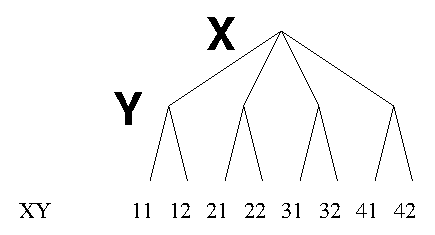
\epsfig{file=cimke1.eps,width=0.2\textwidth}}}
\br
{\tt | ?- }\parbox[t]{0.3\textwidth}{\tt
X in 1..4,
Y in 1..2,\\
indomain(Y),\\
indomain(X).
}\raisebox{-1.5ex}{\parbox[c]{0.2\textwidth}{%\vspace*{-1ex}
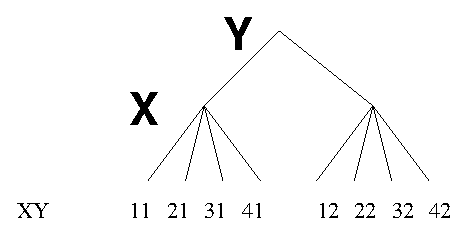
\epsfig{file=cimke2.eps,width=0.2\textwidth}}}
\br
Ha feltételezzük, hogy a fenti keresés során egyes ágak meghiúsulhatnak, akkor könnyen
rájöhetünk, hogy érdemesebb a második ábra szerinti keresési teret választani, mert ha
itt a kezdő csomópontból kimenő egyik ág meghiúsul, akkor azzal már helyből 4 eset
ellenőrzését spóroltuk meg. Ez az úgynevezett \emph{first-fail} elv: előbb címkézzük
a kisebb tartományú változót, ezzel remélhetőleg kevesebb választási pont lesz,
csökken a keresési tér mérete. Az is előfordulhat, hogy egyes feladattípusokhoz saját,
speciális sorrend a célszerű: például az N királynő feladatban célszerű előbb a középső
sorokba elhelyezni a királynőket, mert ezek jobban megszűrik a maradék változók
értékkészletét, mint a szélső sorokba helyezett királynők.
\br
A \clpfd könyvtár beépített címkéző eljárása, a \cd{labeling/2} az első paraméterként
átadott címkézési opció-listán keresztül lehetőséget ad arra, hogy a keresési tér
szerkezetét befolyásoljuk. Három lehetőség közül választhatunk:

\begin{itemize}
\item \emph{Felsorolás (\cd{enum})} --- többszörös választási pontot hoz létre, pontosan
annyi ággal, ahány lehetséges értéke van a változónak. Egy ágon mindig ezen értékek
közül pontosan az egyikre történik behelyettesítés. Használatára példa: \\
\cd{| ?- X in 1..4, labeling([enum],[X]).}
\item \emph{Kettévágás (\cd{bisect})} --- a változó tartományát megfelezi, és két ágat hoz
létre, értelemszerűen a két résztartományra való behelyettesítésével. Használatára példa: \\
\cd{| ?- X in 1..4, labeling([bisect],[X]).}
\item \emph{Lépegetés (\cd{step})} --- kiválaszt a változó tartományából egy értéket,
és két ágat hoz létre. Az egyik ágon erre az értékre szűkíti a változó tartományát,
a másik ágon pedig ezt az értéket kizárja a változó tartományából. Használatára példa: \\
\cd{| ?- X in 1..4, labeling([step],[X]).}
\end{itemize}

Az alábbi ábrákon egy 1..4 értékkészlettel rendelkező változó különböző címkézéseiből
adódó keresési terek láthatóak.

\label{kerfak}
\begin{center}\begin{tabular}{ccc}

\epsfig{file=vpont_enum.eps,width=0.095\textwidth} &
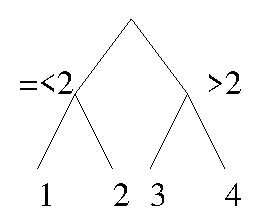
\epsfig{file=vpont_bisect.eps,width=0.1\textwidth} &
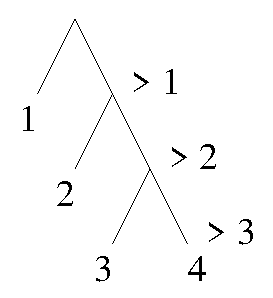
\epsfig{file=vpont_step.eps,width=0.1\textwidth} \\
Felsorolás (\cd{enum}) & Kettévágás (\cd{bisect}) & Lépegetés (\cd{step})
\end{tabular}\end{center}

Ezen ,,rövid'' bevezető után lássuk a \cd{labeling/2} címkéző eljárás részletes
ismertetését!

\enumhead{A címkézés alap-eljárása:
\cd{labeling(Opciók, VáltozóLista)}}

A \cd{VáltozóLista} minden elemét minden lehetséges módon behelyettesíti,
az \cd{Opciók} lista által előírt módon.  Az alábbi csoportok mindegyikéből
legfeljebb egy opció szerepelhet. Hibát jelez, ha a \cd{VáltozóLista}-ban van
nem korlátos tartományú változó. Ha az első négy csoport valamelyikéből nem
szerepel opció, akkor a {\tt\em dőlt betűvel} szedett alapértelmezés lép életbe.

\begin{enumerate}
\item a változó kiválasztása: \cd{{\em leftmost}, min, max, ff, ffc,
variable(Sel)}. Ezek jelentése:
	\begin{itemize}
	\item \cd{leftmost} --- a változólista legbaloldalibb eleme.
	\item \cd{min} --- a legkisebb alsó határú. Ha több van, akkor ezek közül
	a legbaloldalibb.
	\item \cd{max} --- a legnagyobb felső határú. Ha több van, akkor ezek közül
	a legbaloldalibb.
	\item \cd{ff} --- \emph{first-fail} elv szerint a legkisebb tartományú
	(ld. \cd{fd_size/2} az \ref{fdset}. fejezetben). Ha több van, akkor ezek közül
	a legbaloldalibb.
	\item \cd{ffc} --- a legkisebb tartományú. Ha több ilyen van, akkor ezek
    	közül az, amelyikhez a legtöbb korlát kapcsolódik (\emph{most constrained} elv).
	Ha még mindig több ilyen van, akkor ezek közül a legbaloldalibb. Egy változóhoz
	kapcsolódó korlátok számát az \cd{fd_degree/2} adja meg (ld. \ref{fdset}. fejezet).
	\item \cd{variable(Sel)} --- testreszabott változó-kiválasztás: a következő
	változó kiválasztása a \cd{Sel} felhasználói eljárás szerint történik. Bővebben
	erről a \pageref{variable:sel}. oldalon még lesz szó.
	\end{itemize}
\item a választási pont fajtája: \cd{{\em step}, enum, bisect, value(Enum)}. Ezek
jelentése:
	\begin{itemize}
	\item \cd{step} --- \cd{X \#= B} és \cd{X \#\bs= B} közti választás, ahol
	\cd{B} az \cd{X} tartományának alsó vagy felső határa, a bejárási iránytól
	függően
	\item \cd{enum} --- többszörös választás \cd{X} lehetséges értékei közül
	\item \cd{bisect} --- \cd{X \#< M} és \cd{X \#>= M} közti választás, ahol
	\cd{M} az \cd{X} tartományának középső eleme.
	\item \cd{value(Enum)} --- testreszabott választás: \cd{Enum} egy felhasználói
	eljárás, amelynek szerepe, hogy leszűkítse X tartományát. Bővebben erről
	az \pageref{value:enum}. oldalon még lesz szó.
	\end{itemize}
\item a bejárási irány: \cd{{\em up}, down}. \cd{up} értelemszerűen alulról felfelé,
\cd{down} felülről lefelé járja be a tartományt. Csak \cd{step} típusú
címkézésnél van szerepe.
\item a keresett megoldások: \cd{{\em all}, minimize(X), maximize(X)}. Ezek jelentése:
	\begin{itemize}
	\item \cd{all} -- az összes megoldást megkeresi
	\item \cd{minimize(X)} -- azt a megoldást adja vissza, melyben \cd{X} értéke
	minimális.
	\item \cd{maximize(X)} -- azt a megoldást adja vissza, melyben \cd{X} értéke
	maximális.
	\end{itemize}
\item a gyűjtendő statisztikai adat: \cd{assumptions(A)}. A keresés végén egyesíti
\cd{A} értékét a sikeres megoldáshoz vezető ágon lévő változó-kiválasztások
számával (ami lényegében a keresési út hosszát jelenti).
\item a balszélső ágtól való eltérés korlátozása: \cd{discrepancy(D)}. Ezzel azt
korlátozzuk, hogy a keresés során maximum \cd{D}-szer választhatunk a választási
pontokban nem legbaloldalibb ágat. Akkor hasznos, ha a probléma megoldására van
valamiféle heurisztikánk, és úgy alakítjuk ki a keresési teret, hogy a heurisztika
szerinti optimális választást a legbaloldalibb ág tartalmazza. Mivel a heurisztika
nem teljesen tökéletes, ezért valamekkora eltérést megengedünk (ezt szabályozzuk
\cd{D} értékével). Ezt a módszert hívjuk \emph{Limited Discrepancy Search}-nek (LDS).
\end{enumerate}

A fenti pontokra való hivatkozással a \cd{labeling/2} eljárás pontos működése
így fest:

\label{labeling:lepesek}
\begin{description}
\item[a.]  Ha a változólista üres, akkor a címkézés sikeresen véget
ér. Egyébként kiválasztunk belőle egy \cd{X} elemet az 1. csoportbeli opció
által előírt módon.
\item[b.] Ha \cd{X} behelyettesített, akkor a változólistából elhagyjuk, és az
{\bf a.} pontra megyünk.
\item[c.] Egyébként az \cd{X} változó tartományát felosztjuk két vagy több
diszjunkt részre a 2. csoportbeli opció szerint (kivéve \cd{value(Enum)}
esetén, amikor is azonnal az {\bf e.} pontra megyünk).
\item[d.] A tartományokat elrendezzük a 3. csoportbeli opció szerint.
\item[e.] Létrehozunk egy választási pontot, amelynek ágain sorra
leszűkítjük az \cd{X} változót a kiválasztott tartományokra.
\item[f.] Minden egyes ágon az \cd{X} szűkítése értelemszerűen kiváltja a
rá vonatkozó korlátok felébredését. Ha ez meghiúsulást okoz, akkor
visszalépünk az {\bf e.} pontra és ott a következő ágon folytatjuk.
\item[g.] Ha \cd{X} most már behelyettesített, akkor elhagyjuk a változólistából.
Ezután mindenképpen folytatjuk az {\bf a.} pontnál.
\item[h.] Eközben értelemszerűen követjük a 4-6. csoportbeli opciók előírásait is.
\end{description}

Lássunk egy példát az \fdbg nyomkövető könyvtár (\ref{fdbg}. fejezet) használatával!
\br
\begin{verbatim}
| ?- fdbg_assign_name(X, x), fdbg_assign_name(Y, y),
     X in 1..3, Y in 1..2, X #>= Y, fdbg_on,
     labeling([min], [X,Y]).
% The clp(fd) debugger is switched on
Labeling [1, <x>]: starting in range 1..3.
Labeling [1, <x>]: step: <x> = 1
    <y>#=<1     y = 1..2 -> {1} Constraint exited.
                                                X = 1, Y = 1 ? ;
Labeling [1, <x>]: step: <x> >= 2
    <y>#=<<x>   y = 1..2, x = 2..3  Constraint exited.
    Labeling [6, <y>]: starting in range 1..2.
    Labeling [6, <y>]: step: <y> = 1
        Labeling [8, <x>]: starting in range 2..3.
        Labeling [8, <x>]: step: <x> = 2
                                                X = 2, Y = 1 ? ;
        Labeling [8, <x>]: step: <x> >= 3
                                                X = 3, Y = 1 ? ;
        Labeling [8, <x>]: failed.
    Labeling [6, <y>]: step: <y> >= 2
        Labeling [12, <x>]: starting in range 2..3.
        Labeling [12, <x>]: step: <x> = 2
                                                X = 2, Y = 2 ? ;
        Labeling [12, <x>]: step: <x> >= 3
                                                X = 3, Y = 2 ? ;
        Labeling [12, <x>]: failed.
    Labeling [6, <y>]: failed.
Labeling [1, <x>]: failed.
\end{verbatim}

A keresési fa:

\begin{center}
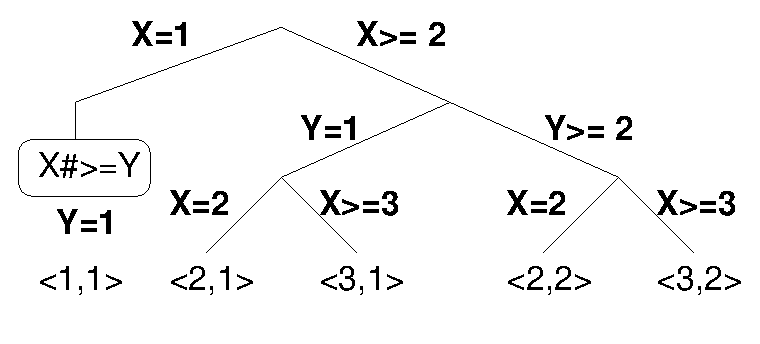
\epsfig{file=cimke_pelda.eps,width=0.4\textwidth}
\end{center}

Egy másik példa, ezúttal szélsőérték-számításra:

\begin{verbatim}
| ?- _L=[X,Y,Z], domain(_L, 0, 1), V#=Y+Z-X, labeling([minimize(V)], _L).
V = -1, X = 1, Y = 0, Z = 0 ? ;
no
\end{verbatim}

A keresési fa (branch-and-bound algoritmussal):

\begin{center}
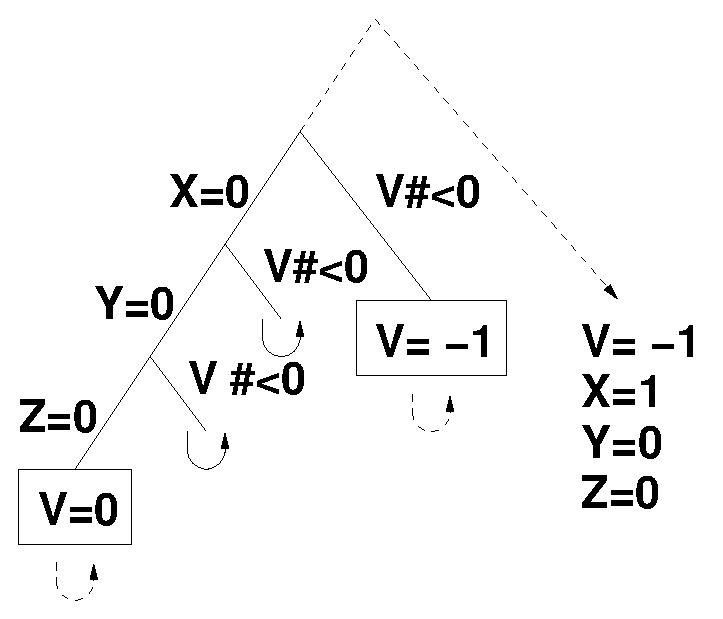
\epsfig{file=bb-pelda.eps,width=0.4\textwidth}
\end{center}

A branch-and-bound algoritmus itt először megkeresi az első megoldást, majd innentől
kezdve a további ágak végigjárása során korlátként felveszi azt is, hogy a megoldásnak
kisebbnek kell lennie, mint az eddig megtalált legkisebb. Ha ezzel a feltétellel is
talál újabb megoldást, akkor innentől kezdve a többi ágon már ezzel az újabb minimummal
dolgozik, egészen addig, amíg be nem járja a teljes keresési teret.
\br
A statisztikai funkciót  és a bal szélső ágtól való eltérés korlátozását bemutató példa
(érdemes összevetni az eredményeket a \pageref{kerfak}. oldalon látható keresési
fákkal):

\begin{alltt}
% a Select címkézési mód használatával megkeresi az X in 1..4 korlát összes
% megoldását, és a megoldásokhoz vezető utak hosszát As-ben adja vissza
assumptions(Select, As) :-
     X in 1..4, findall(A, labeling([Select, assumptions(A)], [X]), As).

% a Select címkézési mód és D eltérés-korlát használatával megkeresi az
% X in 1..4 korlát összes megoldását, és a megtalált megoldásokat visszaadja
% Xs-ben
lds(Select, D, Xs) :-
     X in 1..4, findall(X, labeling([Select, discrepancy(D)], [X]), Xs).

| ?- assumptions(enum, As).          As = [1,1,1,1] ? ; no
| ?- assumptions(bisect, As).        As = [2,2,2,2] ? ; no
| ?- assumptions(step, As).          As = [1,2,3,3] ? ; no

| ?- lds(enum, 1, Xs).               Xs = [1,2,3,4] ? ; no
| ?- lds(bisect, 1, Xs).             Xs = [1,2,3] ? ; no
| ?- lds(step, 1, Xs).               Xs = [1,2] ? ; no
\end{alltt}

Látható, hogy \cd{enum} címkézési módnál minden megoldáshoz 1 hosszú út vezet,
mivel egy többszörös választási pontot hoztunk létre. Éppen ezért az a korlátozásunk,
hogy a legbaloldalibb ágtól maximum egyszer térhetünk el, nem jelent semmi pluszt,
mind a négy megoldást meg tudjuk így keresni.
\br
\cd{bisect} címkézésnél minden megoldáshoz egy 2 hosszú út vezet, hiszen az
első választási pontban az \cd{X \#< 3} és \cd{X \#>= 3} korlátok felvétele között
választunk, a második választási pontban pedig a megmaradó 2 méretű tartományokat
felezzük tovább. A legbaloldalibb ágtól való eltérésre vonatkozó korlátunk így nem
találja meg a 4-et, mint megoldást, mert ahhoz először az \cd{X \#>= 3} ágat, másodszor
pedig az \cd{X = 4} ágat kéne választanunk, és mindkettő jobb oldali ág.
\br
\cd{step} címkézésnél az 1-hez, mint megoldáshoz 1 hosszú út vezet, mert az első
választási pontban az \cd{X = 1} és \cd{X \#= 1} korlátok között döntünk. A 2-t így
már csak két lépésben tudjuk megtalálni, a 3-at és a 4-et pedig hasonló módon csak
3-3 lépésben. Mivel a bal oldali út itt mindig az \cd{X} valamely értékre való kötését
jelenti, és csak egyszer léphetünk jobb oldalra, ezért csak az 1-et és a 2-t fogjuk
megtalálni, hiszen a 3-hoz már kétszer, a 4-hez már háromszor kéne jobbra lépnünk.
\br
\label{variable:sel}
Mint azt már néhány oldallal előbb említettük, a felhasználónak a \cd{labeling/2}
eljárás \cd{variable(Sel)} opcióján keresztül lehetősége van egy saját változó-kiválasztó
eljárás írására is. Az eljárást \cd{Sel(Vars, Selected, Rest)} alakban hívja meg a rendszer,
ahol \cd{Vars} a még címkézendő változók/számok listája. \cd{Sel} feladata, hogy
determinisztikusan egyesítse \cd{Selected}-et a következő címkézendő \emph{változóval},
\cd{Rest}-et pedig a maradékkal. \cd{Sel} egy tetszőleges meghívható kifejezés lehet,
a három argumentumot a rendszer fűzi \cd{Sel} argumentumainak végére, így a \cd{Sel}
által hivatkozott eljárás akár 3-nál több paraméterrel is rendelkezhet. A példa egy olyan
kiválasztást valósít meg, ahol a felhasználó szabályozhatja, hogy hányadik változót
válasszuk ki a változó-listából.

\begin{verbatim}
% A Vars-beli változók között Sel a Hol-adik, ha a lista teljes hosszát
% 1-nek vesszük (Hol így egy törtszám). Rest a maradék.
valaszt(Hol, Vars, Sel, Rest) :-
        szur(Vars, Szurtek),
        length(Szurtek, Len), N is integer(Hol*Len),
        nth0(N, Szurtek, Sel, Rest).

% szur(Vk, Szk): A Vk-ban levő változók listája Szk.
szur([], []).
szur([V|Vk], Szk) :- nonvar(V), !, szur(Vk, Szk).
szur([V|Vk], [V|Szk]) :- szur(Vk, Szk).
\end{verbatim}

\label{value:enum}
Lehetőség van a kiválasztott változó tartományának szűkülését is befolyásolni. Ehhez a
\cd{labeling/2} opció-listájában a \cd{value(Enum)} opciót kell megadnunk. \cd{Enum}-ot
a rendszer \cd{Enum(X, Rest, BB0, BB)} alakban hívja meg, ahol \cd{[X|Rest]} a címkézendő
változók listája, és ebből \cd{X}-et kell az eljárásnak címkéznie, mégpedig
nemdeterminisztikus módon \cd{X} tartományát az összes kívánt módon szűkítve (tehát
a \cd{value(Enum)} a \pageref{labeling:lepesek}. oldalon lévő lépések közül a
{\bf c.}, {\bf d.} és {\bf e.} lépéseket váltja ki). \cd{BB} és \cd{BB0} értéke számunkra
csak annyiból lényeges, hogy az első választásnál meg kell hívni \cd{first_bound(BB0, BB)}-t,
a másodiknál pedig \cd{later_bound(BB0, BB)}-t a branch-and-bound, illetve LDS módszerek
kiszolgálására. \cd{Enum} egy meghívható kifejezés, a 4 paramétert a rendszer fűzi \cd{Enum}
argumentumlistájának végére. Példaként tekintsünk egy olyan címkéző eljárást, amely
az értékeket az értéklistában belülről kifelé haladva sorolja fel:

\begin{verbatim}
midout(X, _Rest, BB0, BB) :-
        fd_size(X, Size),
        Mid is (Size+1)//2,
        fd_set(X, Set),
        fdset_to_list(Set, L),
        nth(Mid, L, MidElem),
        (   first_bound(BB0, BB), X = MidElem
        ;   later_bound(BB0, BB), X #\= MidElem
        ).

| ?- X in {1,3,12,19,120},
     labeling([value(midout)], [X]).
X = 12 ? ;
X = 3 ? ;
X = 19 ? ;
X = 1 ? ;
X = 120 ? ; no
\end{verbatim}

Végül, a címkézés testreszabásának fontosságát bizonyítandó, nézzük meg az N királynő
feladat megoldását különféle címkéző módszerekkel (600 MHz-es Pentium III gépen):

\begin{center}
\enumhead{Összes megoldás keresése}
\begin{tabular}{|l|rr|rr|rr|}
\hline
méret           & \multicolumn{2}{c|}{ n=8}    & \multicolumn{2}{c|}{ n=10}    & \multicolumn{2}{c|}{ n=12}    \\
\hline
megoldások száma       & \multicolumn{2}{c|}{92}    & \multicolumn{2}{c|}{
724}    & \multicolumn{2}{c|}{ 14200}    \\
\hline
címkézés                     & sec & btrk & sec & btrk & sec & btrk \\
\hline
\hline
\cd{[step]}                 & 0.07 & 324 & 1.06 & 5942 & 25.39 & 131K \\ \hline
\cd{[enum]}                 & 0.07 & 324 & 1.03 & 5942 & 24.84 & 131K \\ \hline
\cd{[bisect]}               & 0.07 & 324 & 1.07 & 5942 & 26.04 & 131K \\ \hline \hline
\cd{[enum,min]}             & 0.08 & 462 & 1.31 & 8397 & 33.89 & 202K \\ \hline
\cd{[enum,max]}             & 0.07 & 462 & 1.31 & 8397 & 33.89 & 202K \\ \hline
\cd{[enum,ff]}              & 0.06 & 292 & 0.97 & 4992 & 21.57 & 101K \\ \hline
\cd{[enum,ffc]}             & 0.06 & 292 & 1.04 & 4992 & 23.24 & 101K \\ \hline
\cd{[enum,{\em midvar}\footnotemark[1]]\footnotemark[2]}    & 0.06 & 286 & 0.90 & 4560 & 20.11 &  88K \\ \hline
\end{tabular}
\end{center}

\begin{center}
\enumhead{Első megoldás keresése}
\begin{tabular}{|l|rr|rr|rr|}
\hline
méret           & \multicolumn{2}{c|}{ n=16}    & \multicolumn{2}{c|}{ n=18}    & \multicolumn{2}{c|}{ n=20}    \\
\hline
címkézés                     & sec & btrk & sec & btrk & sec & btrk \\
\hline
\hline
\cd{[enum]}                 & 0.43 & 1833 & 1.76 &  7436 &  9.01 & 37320\\ \hline
\cd{[enum,min]}             & 0.52 & 2095 & 0.87 &  2595 &  1.39 &  3559\\ \hline
\cd{[enum,max]}             & 0.61 & 3182 & 2.68 & 13917 & 16.06 & 83374\\ \hline
\cd{[enum,ff]}              & 0.03 &    7 & 0.05 &    11 &  0.08 &    33\\ \hline
\cd{[enum,ffc]}             & 0.03 &    7 & 0.05 &    11 &  0.09 &    33\\ \hline
\cd{[enum,{\em midvar\footnotemark[1]}]\footnotemark[2]}    & 0.04 &   69 & 0.06 &    57 &  0.15 &   461\\ \hline
\cd{[value(midout)\footnotemark[2]]}        & 0.04 &    3 & 0.05 &     4 &  0.09 &    38\\ \hline
\cd{[value(midout)\footnotemark[2],ffc]}    & 0.04 &   15 & 0.06 &    41 &  0.08 &    20\\ \hline
\end{tabular}
\end{center}

\footnotetext[1]{{\tt{\em midvar} $\equiv$ variable(valaszt(0.5))}.}
\footnotetext[2]{Hatékonyabb statikusan (a címkézés előtt egyszer) elrendezni a változókat
és az értékeket, \\ lásd az {\tt alt_queens/2} eljárást a \cd{library('clpfd/examples/queens')} állományban.}

%% bele kéne venni a 91. oldalon lévő részt is???? (szélsőértékek ismételt hívással való
%% előállítása témakör)

\section{Kombinatorikus korlátok}

Az ebben a fejezetben ismertetett globális korlátok az eddigiekhez hasonlóan
nem tükrözhetőek. Minden olyan helyen, ahol a korlátok FD-változót várnak,
írhatunk számértéket is.

\subsection{Értékek számolása és különbözősége}

\medskip

{\bcd{count(Val, List, {\em Relop}, Count)}}

Jelentése: a \cd{Val} egész szám a \cd{List} FD-változó-listában $n$-szer fordul elő,
és fennáll az  {\it n} \cd{{\em Relop} Count} reláció. Itt \cd{Count} FD változó,
\cd{\em Relop} pedig a hat összehasonlító reláció egyike: \cd{\#=, \#\bs=, \#<} \ldots.
Tartomány-szűkítést biztosít.

\medskip

{\bcd{global_cardinality(Vars, Vals)}}

\cd{Vars} egy FD változókból álló lista, \cd{Vals} pedig  \cd{I-K} alakú párokból
álló lista, ahol \cd{I} egy egész, \cd{K} pedig egy FD változó. Mindegyik \cd{I}
érték csak egyszer fordulhat elő a \cd{Vals} listában. Jelentése: A \cd{Vars}-beli
FD változók csak a megadott \cd{I} értékeket vehetik fel, és minden egyes \cd{I-K}
párra igaz, hogy a \cd{Vars} listában pontosan \cd{K} darab \cd{I} értékű elem van.
Ha \cd{Vals} vagy \cd{Vars} tömör, és még sok más speciális esetben tartomány-szűkítést
ad.

\medskip

\label{all_distinct}
{\bcd{all\_different(Vs{\em [}, Options{\em ]})\\
      all\_distinct(Vs{\em [}, Options{\em ]})}}

Jelentése: a \cd{Vs} FD változó-lista elemei páronként különbözőek.
A korlát szűkítési mechanizmusát az \cd{Options} opció-lista szabályozza,
eleme lehet:

\begin{itemize}
\item \cd{consistency(Cons)} --- a szűkítési algoritmust szabályozza. \cd{Cons} lehet:
\begin{description}
\item[\cd{global}] --- tartomány-szűkítő algoritmus (Regin), durván a
tartományok méretével arányos idejű (alapértelmezés \cd{all\_distinct} esetén)
\item[\cd{bound}] --- intervallum-szűkítő algoritmus (Mehlhorn), a
változók és értékek számával arányos idejű
\item[\cd{local}] --- a nemegyenlőség páronkénti felvételével azonos
szűkítő erejű algoritmus, durván a változók számával arányos idejű
(alapértelmezés \cd{all\_different} esetén).
\end{description}

\item \cd{on(On)} --- az ébredést szabályozza. \cd{On} lehet:
\begin{description}
\item[\cd{dom}] --- a változó tartományának bármiféle változásakor
ébreszt (alapértelmezés \cd{all\_distinct} esetén),
\item[{\rm \bf \cd{min}, \cd{max}, {\rm ill.} \cd{minmax}}] ---
a változó tartományának adott ill. bármely határán történő változáskor ébreszt,
\item[\cd{val}] --- a változó behelyettesítésekor ébreszt csak (alapértelmezés
\cd{all\_different} esetén).
\end{description}

A \cd{consistency(local)} beállításnál nincs értelme \cd{val}-nál
korábban ébreszteni, mert ez a szűkítést nem befolyásolja.
\end{itemize}

A különböző ébresztési és szűkítési módok bemutatásához nézzük az alábbi predikátumot:

\begin{verbatim}
pelda(Z, I, On, C) :-
     L = [X,Y,Z], domain(L, 1, 3),
     all_different(L, [on(On),consistency(C)]), X #\= I, Y #\= I.
\end{verbatim}

\begin{tabular}{ll}
\verb'| ?- pelda(Z, 3, dom, local).'    & $\rightarrow$ \verb'  Z in 1..3 '  \\
\verb'| ?- pelda(Z, 3, min, global).'   & $\rightarrow$ \verb'  Z in 1..3 '  \\
\verb'| ?- pelda(Z, 3, max, bound).'    & $\rightarrow$ \verb'  Z = 3     '  \\
\verb'| ?- pelda(Z, 2, minmax, global).'& $\rightarrow$ \verb'  Z in 1..3 '  \\
\verb'| ?- pelda(Z, 2, dom, bound).'    & $\rightarrow$ \verb'  Z in 1..3 '  \\
\verb'| ?- pelda(Z, 2, dom, global).'   & $\rightarrow$ \verb'  Z = 2     '  \\
\end{tabular}
\br
Látható, hogy csak a harmadik és a hatodik példa jön rá arra, hogy \cd{Z} csak
a második paraméterben megadott érték lehet. Az első és az ötödik példa a \cd{local},
illetve \cd{bound} algoritmus gyengesége miatt nem végzi el a szűkítést, a második
és a negyedik pedig a nem megfelelő ébresztési feltétel miatt.

\subsection{Függvénykapcsolatok és relációk}

{\bcd{element(X, List, Y)}}

Jelentése: \cd{List} \cd{X}-edik eleme \cd{Y} (1-től számozva). Itt \cd{X} és \cd{Y}
FD változók, \cd{List} FD változókból álló lista. Az \cd{X} változóra nézve
tartomány-szűkítést, az \cd{Y} és \cd{List} változókra nézve intervallum-szűkítést
biztosít.

Példák:

\begin{verbatim}
| ?- element(X, [0,1,2,3,4], Y), X in {2,5}.  % ekvivalens Y #= X-1-gyel
X in {2}\/{5}, Y in 1..4 ?                    % intervallum-konzisztens
| ?- element(X, [0,1,2,3,4], Y), Y in {1,4}.
X in {2}\/{5}, Y in {1}\/{4} ?                % tartomány-konzisztens

% X #= C #<=> B megvalósítása, 1=<{X,C}=<6 esetére
% (C konstans).
beq(X, C, B) :-
        X in 1..6, call(I #= X+6-C),
        element(I, [0,0,0,0,0,1,0,0,0,0,0], B).
\end{verbatim}

\medskip
{\bcd{relation(X, Rel, Y)}}

Itt \cd{X} és \cd{Y} FD változók, \cd{Rel} formája: egy lista
{\tt\em Egész-KonstansTartomány} alakú párokból (ahol mindegyik {\tt\em Egész}
csak egyszer fordulhat elő). Jelentése: \cd{Rel} tartalmaz egy \cd{X-Tart} párt,
ahol \cd{Y} eleme a \cd{Tart}-nak, azaz: \[ \cd{relation(X,H,Y)} \equiv \tuple{\cd{X,Y}}
\in \{\tuple{x,y}|x-\cd{T} \in \cd{H}, y \in \cd{T}\}\] Tetszőleges bináris reláció
definiálására használható, tartomány-szűkítést biztosít. Példa:

\begin{verbatim}
'abs(x-y)>1'(X,Y) :-
        relation(X, [0-(2..5), 1-(3..5), 2-{0,4,5},
                     3-{0,1,5}, 4-(0..2), 5-(0..3)], Y).

| ?- 'abs(x-y)>1'(X,Y), X in 2..3.
Y in (0..1) \/ (4..5) ? ;
no
\end{verbatim}

\medskip
{\bcd{case(Template, Tuples, DAG{\em [}, Options{\em ]})}}

Jelentése: A \cd{Tuples} lista minden elemét illesztve a \cd{Template}
mintára, a \cd{DAG} által leírt reláció fennáll. Az ébresztést és a
szűkítést az \cd{Options} opció-lista szabályozza (hasonló módon, mint
az \cd{all_distinct} esetén, lásd \pageref{all_distinct}. oldal és
SICStus kézikönyv). Alaphelyzetben minden változásra ébred és
tartomány-szűkítést ad.

A \cd{DAG} csomópontok listája, az első elem a kezdőpont. Egy csomópont
alakja: \cd{node(ID, X, Successors)}. Itt \cd{ID} a csomópont azonosítója
(egész vagy atom), \cd{X} a vizsgálandó változó. Belső gráfpont esetén
\cd{Successors} a rákövetkező csomópontok listája, elemei \cd{Min..Max)-ID2}
alakúak. Egy ilyen elem jelentése: ha \cd{Min} $\leq$ \cd{X} $\leq$ \cd{Max},
akkor menjünk az \cd{ID2} csomópontra. Végpont esetén \cd{Successors} a
végfeltételek listája, elemei \cd{Min..Max} alakúak, jelentése pedig: ha
valamelyik elem esetén \cd{Min} $\leq$ \cd{X} $\leq$ \cd{Max} fennáll, akkor
a reláció teljesül.
\br
Példaként tekintsük az alábbi gráfot, amely az ,,\cd{X}, \cd{Y} és \cd{Z}
felének egészrésze mind más'' (\([\frac{\cd{X}}{\cd{2}}]\neq[\frac{\cd{Y}}{\cd{2}}],
[\frac{\cd{X}}{\cd{2}}]\neq[\frac{\cd{Z}}{\cd{2}}],
[\frac{\cd{Y}}{\cd{2}}]\neq[\frac{\cd{Z}}{\cd{2}}]\)) relációt írja le a 0..5
tartományon:

\begin{center}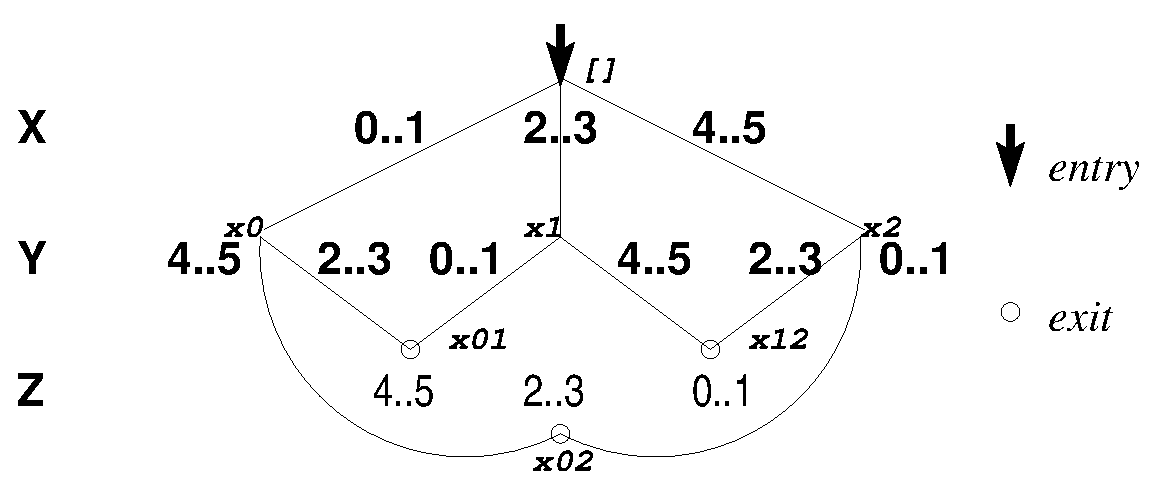
\epsfig{file=case.eps,width=0.7\textwidth}\end{center}

Ennek megvalósítása a \cd{case/3} korláttal:

\begin{verbatim}
felemasok(X, Y, Z) :-
   case(f(A,B,C), [f(X,Y,Z)],
        [node([], A, [(0..1)-x0,(2..3)-x1,(4..5)-x2]),
         node(x0, B, [(2..3)-x01,(4..5)-x02]),
         node(x1, B, [(0..1)-x01,(4..5)-x12]),
         node(x2, B, [(0..1)-x02,(2..3)-x12]),
         node(x01,C,[4..5]), node(x02,C,[2..3]), node(x12,C,[0..1])
        ]).
\end{verbatim}

Példa többszörös mintára: \cd{case(T,[A$_1$,$\ldots$],D)$\equiv$case(T,[A$_1$],D),$\ldots$}

\begin{verbatim}
felemasok_vacak(X, Y, Z) :-
    case(A\=B, [X\=Y,X\=Z,Y\=Z],
     [node(root, A, [(0..1)-0,(2..3)-1,(4..5)-2]),
      node(0,B,[2..5]),node(1,B,[0..1,4..5]),node(2, B, [0..3])
     ], [on(val(X)),on(val(Y)),on(val(Y))/*,prune(val(X)), ...*/]).
\end{verbatim}

\subsection{Leképezések, gráfok}

{\bcd{sorting(X, I, Y)}}

Az \cd{X} FD-változókból álló lista rendezettje az \cd{Y} FD-változó-lista. Az \cd{I}
FD-változó-lista írja le a rendezéshez szükséges permutációt. Azaz: mindhárom
paraméter azonos ($n$) hosszúságú, \cd{Y} rendezett, \cd{I} az \cd{1..$n$} számok
egy permutációja, és $\forall i \in$ \cd{1..$n$} esetén \cd{X$_i$ =Y$_{\cd{I}_i}$}.

\medskip

{\bcd{assignment(X, Y{\em [}, Options{\em ]})}}

\cd{X} és \cd{Y} FD változókból alkotott azonos ($n$) hosszúságú listák. Teljesül,
ha \cd{X$_i$} és \cd{Y$_i$} mind az \cd{1..$n$} tartományban vannak és \cd{X$_i$=$j$}
$\Leftrightarrow$ \cd{Y$_j$=$i$}. Másképpen fogalmazva: \cd{X} egy-egyértelmű
leképezés az \cd{1..$n$} halmazon (az \cd{1..$n$} számok egy permutációja), és
\cd{Y} az \cd{X} inverze.

Az \cd{Options} lista ugyanolyan, mint az \cd{all\_different/[1,2]} korlát
esetében (ld. \pageref{all_distinct}. oldal), az alapértelmezés
\cd{[on(domain),consistency(global)]}.

\medskip

{\bcd{circuit(X)} }

\cd{X} $n$ hosszúságú lista. Igaz, ha minden \cd{X$_i$} az \cd{1..$n$}
tartományba esik, és \cd{X$_1$, X$_{\cd{X}_1}$, X$_{\cd{X}_{\cd{X}_1}}$... }
($n$-szer ismételve) az \cd{1..$n$} számok egy permutációja. Másképp: \cd{X} egy
egyetlen ciklusból álló permutációja az \cd{1..$n$} számoknak.

Gráfokon vett értelmezés: legyen egy $n$ szögpontú irányított gráfunk,
jelöljük a pontokat az \cd{1..$n$} számokkal. Vegyünk fel $n$ db FD-változót,
\cd{X$_i$} tartománya álljon azon $j$ számokból, amelyekre $i$-ből vezet $j$-be él.
Ekkor \cd{circuit(X)} azt jelenti, hogy az $i$ $\rightarrow$ \cd{X$_i$} élek a
gráf egy Hamilton-körét adják.

\medskip

{\bcd{circuit(X, Y)}}

Ekvivalens a következővel: \cd{circuit(X), assignment(X, Y)}. Gráfokon értelmezve
megadja a Hamilton-kört és annak az ellenkező irányban vett bejárását is.

Példák az \cd{assignment/2} és a \cd{circuit/2} használatára:

\begin{verbatim}
| ?- length(L, 3), domain(L, 1, 3), assignment(L, LInv), L=[2|_],
     labeling([], L).
L = [2,1,3], LInv = [2,1,3] ? ;
L = [2,3,1], LInv = [3,1,2] ? ;
no
| ?- length(L, 3), domain(L, 1, 3), circuit(L, LInv), L=[2|_].
L = [2,3,1], LInv = [3,1,2] ? ;
no
\end{verbatim}

Kicsit ,,életszagúbb'' példa:

\medskip

\begin{tabular}{cp{0.8\textwidth}}
\begin{tabular}{|c|c|c|}
\hline 1 & 2 & 2 \\ \hline 3 & 1 & 3 \\ \hline 4 & 4 & 1 \\ \hline
\end{tabular} &
\vspace{-1.5\baselineskip}
Adott a bal oldalt látható 3 $\times$ 3-as négyzetrács. Feladat: járjuk be
a rács elemeit a bal felső sarokból indulva úgy, hogy minden cellán pontosan
egyszer haladunk át, és $n$-t tartalmazó celláról csak $n+1$-et tartalmazóra
léphetünk (kivéve $n=4$ esetben, innen csak 1-est tartalmazóra). \\
\end{tabular}

\begin{verbatim}
| ?- L=[_1,_2,_3,_4,_5,_6,_7,_8,1], _1=2, _2 in {4,6}, _3=6,
     _4 in {7,8}, _5 in {2,3}, _6=8, _7=5, _8 in {5,9},
     circuit(L).
L = [2,4,6,7,3,8,5,9,1] ? ; no
\end{verbatim}

Az eredmény-listában minden elem megadja, hogy az elemnek megfelelő cella után
melyik cella következik a körben (a cellákat fentről lefelé és balról jobbra
számoztuk be 1-től 9-ig).
\br
A \cd{circuit/1} felhasználható az utazó ügynök probléma megoldására is:

\begin{verbatim}
:- module(tsp, [tsp/3]).
:- use_module(library(clpfd)).
:- use_module(library(lists), [append/3]).

tsp(Lab, Successor, Cost) :-
        Successor = [X1,X2,X3,X4,X5,X6,X7],
        Costs = [C1,C2,C3,C4,C5,C6,C7],
        element(X1, [0,205,677,581,461,878,345], C1),
        element(X2, [205,0,882,427,390,1105,540], C2),
        element(X3, [677,882,0,619,316,201,470], C3),
        element(X4, [581,427,619,0,412,592,570], C4),
        element(X5, [461,390,316,412,0,517,190], C5),
        element(X6, [878,1105,201,592,517,0,691], C6),
        element(X7, [345,540,470,570,190,691,0], C7),
        sum(Costs, #=, Cost),
        Predecessor = [Y1,Y2,Y3,Y4,Y5,Y6,Y7],
        Costs2 = [D1,D2,D3,D4,D5,D6,D7],
        element(Y1, [0,205,677,581,461,878,345], D1),
        element(Y2, [205,0,882,427,390,1105,540], D2),
        element(Y3, [677,882,0,619,316,201,470], D3),
        element(Y4, [581,427,619,0,412,592,570], D4),
        element(Y5, [461,390,316,412,0,517,190], D5),
        element(Y6, [878,1105,201,592,517,0,691], D6),
        element(Y7, [345,540,470,570,190,691,0], D7),
        sum(Costs2, #=, Cost),
        circuit(Successor, Predecessor),
        append(Successor, Predecessor, All),
        labeling([minimize(Cost)|Lab], All).

| ?- tsp([ff], Succs, Cost).
Cost = 2276, Succs = [2,4,5,6,7,3,1] ?
\end{verbatim}

\subsection{Ütemezési korlátok}

{\bcd{cumulative(Starts, Durations, Resources, Limit{\em[}, Opts{\em ]})}}

Jelentése: a \cd{Starts} kezdőidőpontokban elkezdett, \cd{Durations} ideig tartó
és \cd{Resources} erőforrásigényű feladatok bármely időpontban összesített
erőforrásigénye nem haladja meg a \cd{Limit} határt (és fennállnak az opcionális
precedencia korlátok). Az első három argumentum FD változókból álló, egyforma ($n$)
hosszú lista, a negyedik egy FD változó.

\medskip

{\bcd{serialized(Starts, Durations{\em [}, Opts{\em ]})}}

A \cd{cumulative} speciális esete, ahol az összes erőforrás-igény és a korlát is 1.

\br
Vezessük be a \cd{cumulative($S,D,R,Lim$ \dots )} híváshoz az alábbi jelöléseket:

\begin{quote}
$a = min(S_1,\ldots,S_n)$ {\rm $a$ a kezdőidőpont)} \\
$b = max(S_1+D_1,\ldots,S_n+D_n)$ {\rm $b$ a (végidőpont)}\\
$R_{ij} = R_j$, ha  $S_j \leq i < S_j+D_j$,
        egyébként $R_{ij} = 0$; {\rm $R_{ij}$ (a $j$. feladat erőforrásigénye
        az $i$. időpontban)}
\end{quote}

Ezekkel a jelölésekkel a korlát jelentése (a precedencia-korlátok nélkül):

\begin{quote}
$R_{i1}+\ldots+R_{in} \leq Lim$ minden $a \leq i < b$ esetén.
\end{quote}

Az \cd{Opts} opciólista a következő beállításokat tartalmazhatja:

\begin{itemize}
\item \cd{precedences(Ps)} ---
          \cd{Ps} egy lista, amely precedencia korlátokat ír le. Elemei a következők
          lehetnek (\cd{I} és \cd{J} feladatok sorszámai, \cd{D} egy pozitív
          egész, \cd{Tart} egy  konstans-tartomány):
\begin{itemize}
\item\cd{d(I,J,D)}, jelentése: $S_\cd{I}+\cd{D} \leq S_\cd{J}$ vagy $S_\cd{J} \leq S_\cd{I}$
(tehát az \cd{I}. és a \cd{J}. feladat közti átállás egy holtidővel modellezhető, és
\cd{D} az \cd{I}. feladat hossza ($D_\cd{I}$) plusz az átállási idő. Ha azt akarjuk
megadni, hogy egy feladatot előbb el kell végezni, mint egy másikat, akkor átállási
időnek \cd{sup}-ot kell megadni.
\item\cd{I-J in Tart}, jelentése: \cd{$S_\cd{I}-S_\cd{J}$ \#= D$_\cd{IJ}$,
D$_\cd{IJ}$ in Tart}. Akkor használatos, ha az \cd{I}. és \cd{J}. feladat között
eltelt időnek alsó és felső korlátja is van.
\end{itemize}

\item \cd{resource(R)} --- speciális ütemezési címkézéshez szükséges opció. \cd{R}-et
          egyesíti egy kifejezéssel, amelyet később átadhatunk az \cd{order\_resource/2}
          eljárásnak, hogy felsoroltassuk a feladatok lehetséges sorrendjeit. Az
          \cd{order_resource/2} eljárásról bővebben a \pageref{order_resource}. oldalon
          lesz szó.

\item \cd{decomposition(Boolean)} ---
          Ha \cd{Boolean} \cd{true}, akkor minden ébredéskor megpróbálja
          kisebb darabokra bontani a korlátot (pl. ha van két
          át nem lapoló feladathalmazunk, akkor ezeket külön-külön
          kezelhetjük, ami az algoritmusok gyorsabb lefutását
          eredményezheti). Alapértelmezésben ki van kapcsolva.

\item \cd{path\_consistency(Boolean)} ---
          Ha \cd{Boolean} \cd{true}, akkor figyeli a feladatok kezdési
          időpontja közti különbségek konzisztenciáját. Ez egy olyan redundáns
          korlátra hasonlít, amely minden $i,j$ párra felveszi a
          \cd{SD$_{ij}$ \#= S$_j$ - S$_i$}, és minden $i,j,k$ hármasra a
          \cd{SD$_{ik}$ \#= SD$_{ij}$ + SD$_{jk}$} korlátot. Alapértelmezésben
          ki van kapcsolva.

\item \cd{static\_sets(Boolean)}
          Ha \cd{Boolean} \cd{true}, akkor, ha bizonyos feladatok sorrendje
          ismert, akkor ennek megfelelően megszorítja azok kezdő
          időpontjait. Alapértelmezésben ki van kapcsolva. Például:
\begin{verbatim}
| ?- _S = [S1,S2,S3],  domain(_S, 0, 9), (SS = false ; SS = true),
     serialized(_S, [5,2,7], [static_sets(SS),
                              precedences([d(3,1,sup), d(3,2,sup)])]).
SS=false, S1 in 0..4, S2 in(0..2)\/(5..7), S3 in 5..9 ? ;
SS=true,  S1 in 0..4, S2 in(0..2)\/(5..7), S3 in 7..9 ? ;
no
\end{verbatim}

\item \cd{edge\_finder(Boolean)}
          Ha \cd{Boolean} \cd{true}, akkor megpróbálja kikövetkeztetni az egyes
          feladatok sorrendjét. Alapértelmezésben ki van kapcsolva. Példa:
\begin{verbatim}
| ?- _S = [S1,S2,S3], domain(_S, 0, 9),
      serialized(_S, [8,2,2], [edge_finder(true)]).
S1 in 4..9, S2 in 0..7, S3 in 0..7 ? ;
no
\end{verbatim}

\item \cd{bounds_only(Boolean)}
          Ha \cd{Boolean} \cd{true}, akkor a korlát az $S_i$ változóknak
          csak a határait szűkíti, a belsejüket nem. Alapértelmezésben be van kapcsolva.

\end{itemize}

\medskip

{\bcd{cumulatives(Tasks, Machines{\em [}, Options{\em ]})}} \\
Több erőforrást (gépet) igénylő feladatok ütemezése (lásd SICStus kézikönyv).
\br
Példaként tekintsünk egy olyan ütemezési feladatot, ahol a rendelkezésre álló
erőforrások száma 13, az erőforrásigények és időtartamok pedig az alábbi táblázat
szerint alakulnak:

\begin{center}
\begin{tabular}{|l|r|r|r|r|r|r|r|}
\hline
Tevékenység               & t1   & t2    & t3   & t4   & t5   & t6   & t7 \\
\hline
Időtartam                 & 16   & 6     & 13   & 7    & 5    & 18   & 4 \\
Erőforrásigény            & 2    & 9     & 3    & 7    &10    & 1    &11\\
\hline
\hline
Egy megoldás              &0--16 &16--22 &9--22 &9--16 &4--9  &4--22 &0--4\\
\hline
\end{tabular}
\end{center}

\begin{verbatim}
% A fenti ütemezési feladatban a tevékenységek kezdőidőpontjait
% az Ss lista tartalmazza, a legkorábbi végidőpont az End.
schedule(Ss, End) :-
        length(Ss, 7),
        Ds = [16, 6,13, 7, 5,18, 4],
        Rs = [ 2, 9, 3, 7,10, 1,11],
        domain(Ss, 0, 30),
        End in 0.. 50,
        after(Ss, Ds, End),
        cumulative(Ss, Ds, Rs, 13),
        labeling([ff,minimize(End)], [End|Ss]).

% after(Ss, Ds, E): Az E időpont az Ss kezdetű Ds időtartamú
% tevékenységek mindegyikének befejezése után van.
after([], [], _).
after([S|Ss], [D|Ds], E) :- E #>= S+D, after(Ss, Ds, E).
\end{verbatim}

\begin{minipage}[c]{0.40\textwidth}
\begin{alltt}
| ?- schedule(Ss, End).

Ss = [0,16,9,9,4,4,0],
End = 22 ? ;
no
\end{alltt}
\end{minipage}
\hspace{0.10\textwidth}
\parbox[c]{0.45\textwidth}{
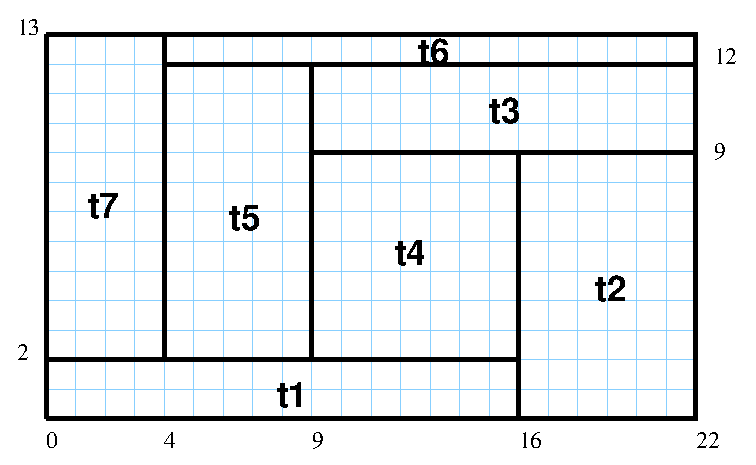
\epsfig{file=sched3.eps,width=0.45\textwidth}}

Példa precedencia-korlátra:

\begin{alltt}
| ?- _S = [S1,S2], domain(_S,0,9), S1 #< S2, {\em{}% a két külön korlát}
     serialized(_S, [4,4], []).              {\em{}% nem jól szűkít:}
        S1 in 0..8, S2 in 1..9 ? ;  no

| ?- _S = [S1,S2], domain(_S,0,9), Opts=[precedences([d(2,1,sup)],
     serialized(_S, [4,4], Opts)]). {\em{}% ^^ \(\equiv\) S1 #< S2}
        S1 in 0..5, S2 in 4..9 ? ;  no
\end{alltt}
\label{order_resource}
{\bcd{order_resource(Options, Resource)}}

Igaz, ha a \cd{Resource} által leírt feladatok elrendezhetők valamilyen
sorrendbe. Ezeket az elrendezéseket felsorolja. A \cd{Resource} argumentumot a
fenti ütemező eljárásoktól kaphatjuk meg az ütemező eljárás opció-listájába
helyezett \cd{resource(Resource)} elemmel. Az \cd{order_resource/2} opció-listája
a következő dolgokat tartalmazhatja (mindegyik csoportból legfeljebb egyet,
alapértelmezés: \cd{[first,est]}):

\begin{itemize}
\item stratégia
     \begin{itemize}
     \item \cd{first} Mindig olyan feladatot választunk ki, amelyet az összes
                       többi elé helyezhetünk.
     \item \cd{last} Mindig olyan feladatot választunk ki, amelyet az összes
                       többi után helyezhetünk.
     \end{itemize}
\item tulajdonság: \cd{first} stratégia esetén az adott tulajdonság
     minimumát, \cd{last} esetén a maximumát tekintjük az összes feladatra
     nézve.
     \begin{itemize}
     \item \cd{est} legkorábbi lehetséges kezdési idő
     \item \cd{lst} legkésőbbi lehetséges kezdési idő
     \item \cd{ect} legkorábbi lehetséges befejezési idő
     \item \cd{lct} legkésőbbi lehetséges befejezési idő
     \end{itemize}
\end{itemize}

Példa:

\begin{verbatim}
| ?- _S=[S1,S2,S3], domain(_S, 0, 9),
     serialized(_S, [5,2,7],
                [precedences([d(3,1,sup), d(3,2,sup)]),
                 resource(_R)]), order_resource([],_R).
S1 in 0..2, S2 in 5..7, S3 in 7..9 ? ;
S1 in 2..4, S2 in 0..2, S3 in 7..9 ? ;
no
\end{verbatim}

Látható, hogy az \cd{order_resource/2} csak a lehetséges elrendezésekre vonatkozóan
címkéz, de az egyes elrendezéseken belül a változók értékeit ,,függőben'' hagyja.

\subsection{Diszjunkt szakaszok és téglalapok}

{\bcd{disjoint1(Lines{\em [}, Options{\em ]})}}

Jelentése: A \cd{Lines} által megadott intervallumok diszjunktak. A \cd{Lines} lista
elemei $F(S_j,D_j)$ vagy $F(S_j,D_j,T_j)$ alakú kifejezések listája, ahol $S_j$ és
$D_j$ $j$. szakasz kezdőpontját és hosszát megadó változók. $F$ tetszőleges funktor,
$T_j$ egy atom vagy egy egész, amely a szakasz típusát definiálja (alapértelmezése 0).
Az \cd{Options} lista a következő dolgokat tartalmazhatja (a \cd{Boolean} változók
alapértelmezése \cd{false}):

\begin{itemize}
\item \cd{decomposition(Boolean)}
          Ha \cd{Boolean} \cd{true}, akkor minden ébredéskor megpróbálja kisebb
          darabokra bontatni a korlátot.

\item \cd{global(Boolean)}
          Ha \cd{Boolean} \cd{true}, akkor egy redundáns algoritmust használ a
          jobb szűkítés érdekében. Példa:

\begin{verbatim}
| ?- domain([S1,S2,S3], 0, 9), (G = false ; G = true),
     disjoint1([S1-8,S2-2,S3-2], [global(G)]).
       G = false, S1 in 0..9, S2 in 0..9, S3 in 0..9 ? ;
       G = true,  S1 in 4..9, S2 in 0..7, S3 in 0..7 ?
\end{verbatim}

\item \cd{wrap(Min,Max)}
          A szakaszok nem egy egyenesen, hanem egy körön helyezkednek el,
          ahol a \cd{Min} és \cd{Max} pozíciók egybeesnek (\cd{Min} and
          \cd{Max} egészek kell, hogy legyenek). Ez az opció a \cd{Min..(Max-1)}
          intervallumba kényszeríti a kezdőpontokat.

\item \cd{margin(T1,T2,D)}
          Bármely \cd{T1} típusú vonal végpontja legalább \cd{D} távolságra lesz
          bármely \cd{T2} típusú vonal kezdőpontjától, ha \cd{D} egész.
          Ha \cd{D} nem egész, akkor a \cd{sup} atomnak kell lennie, ekkor
          minden \cd{T2} típusú vonalnak előrébb kell lennie, mint bármely
          \cd{T1} típusú vonal.
\end{itemize}

{\bcd{disjoint2(Rectangles{\em [}, Options{\em ]})}}

     Jelentése: A \cd{Rectangles} által megadott téglalapok nem metszik
     egymást. A \cd{Rectangles} lista elemei $F(S_{j1},D_{j1},S_{j2},D_{j2})$
     vagy $F(S_{j1},D_{j1},S_{j2},D_{j2},T_j)$ alakú kifejezések. Itt
     $S_{j1}$ és $D_{j1}$ a $j$. téglalap X irányú kezdőpontját és hosszát
     jelölő változók, $S_{j2}$ és $D_{j2}$ ezek Y irányú megfelelői,
     $F$ tetszőleges funktor,  $T_j$ egy egész vagy atom, amely a
     téglalap típusát jelöli (alapértelmezése 0).

Az \cd{Options} lista a következő dolgokat tartalmazhatja (a \cd{Boolean} változók
alapértelmezése \cd{false}):

\begin{itemize}
\item \cd{decomposition(Boolean)}
          Mint \cd{disjoint1/2}.

\item \cd{global(Boolean)}
          Mint \cd{disjoint1/2}.

\item \cd{wrap(Min1,Max1,Min2,Max2)}
          \cd{Min1} és \cd{Max1} egész számok vagy rendre az \cd{inf} vagy
          \cd{sup} atom. Ha egészek, akkor a téglalapok egy olyan henger
          palástján helyezkednek el, amely az X irányban fordul körbe, ahol
          a \cd{Min1} és \cd{Max1} pozíciók egybeesnek. Ez az opció a
          \cd{Min1..(Max1-1)} intervallumba kényszeríti az $S_{j1}$ változókat.
          \cd{Min2} és \cd{Max2} ugyanezt jelenti Y irányban. Ha mind a négy
          paraméter egész, akkor a téglalapok egy tóruszon helyezkednek el.

\item \cd{margin(T1,T2,D1,D2)}
          Ez az opció minimális távolságokat ad meg, \cd{D1} az X,
          \cd{D2} az Y irányban bármely \cd{T1} típusú téglalap vég- és bármely \cd{T2}
          típusú téglalap kezdőpontja között. \cd{D1} és \cd{D2} egészek vagy a
          \cd{sup} atom. \cd{sup} azt jelenti, hogy a \cd{T2} típusú téglalapokat
          a \cd{T1} típusú téglalapok elé kell helyezni a megfelelő irányban.

\item \cd{synchronization(Boolean)}:  Speciális esetben redundáns korlátot
          vesz fel (lásd SICStus kézikönyv).
\end{itemize}

Példa: helyezzünk el három diszjunkt téglalapot úgy, hogy $(x,y)$ bal alsó sarkuk
az $0 \leq x \leq 2, 0 \leq y \leq 1$ téglalapban legyen. A méretek ($x \times y$
sorrendben): 1 $\times$ 3, 2 $\times$ 2, 3 $\times$ 3. Az 1 $\times$ 3-as téglalap
$x$ koordinátája nem lehet 2.

\begin{verbatim}
| ?- domain([X1,X2,X3], 0, 2), domain([Y1,Y2,Y3], 0, 1), X1 #\= 2,
     disjoint2([r(X1,3,Y1,1),r(X2,2,Y2,2),r(X3,3,0,3)]).
X1 in 0..1, Y1 = 0,   X2 = 0, Y2 = 1,   X3 = 2, Y3 = 1 ?
\end{verbatim}

\section{Felhasználói korlátok definiálása}

A SICStus Prolog kétféle lehetőséget kínál a \clpfd modul korlátainak
felhasználói korlátokkal való bővítésére: a \emph{globális korlát}okat és
az \emph{FD predikátum}okat. A \emph{globális korlát}ok tetszőleges (nem korlátos)
számú változót tartalmazó korlátok definiálására alkalmasak. A korlátok
működését teljesen általános Prolog kódként adhatjuk meg, beleértve az
ébresztési feltételeket és a befejezés módját is. A globális korlátok
reifikációja (tükrözése) azonban nem támogatott. Az \emph{FD predikátumok}
ezzel szemben csak rögzített számú változót tartalmazó korlátok leírására
alkalmasak, viszont itt a reifikáció is támogatott, és az ébresztési
feltételek meghatározása automatikus. Az FD predikátumokban a programozó
úgynevezett \emph{indexikálisok} segítségével írja le a szűkítési, illetve
levezethetőségi feltételeket. Az indexikálisok nyelve egy speciális, halmazértékű
funkcionális nyelv a tartományokkal való műveletek végzésére. Az alábbi
Prolog kód egy példa egy FD predikátumra:

\begin{alltt}
% Az X+Y #= T korlát (intervallum szűkítéssel)
'x+y=t'(X,Y,T) +:
        X in min(T) - max(Y)..max(T) - min(Y),
        Y in min(T) - max(X)..max(T) - min(X),
        T in min(X) + min(Y)..max(X) + max(Y).
\end{alltt}

Az indexikális nyelv bővebb elemzése az \ref{fdpred}. fejezetben olvasható.

\subsection{Globális korlátok}

\label{globalis}

Mint azt már említettük, a globális korlátot egy külön Prolog eljárásként
kell megírni, amelyben az \cd{fd\_global/3} eljárással indul el a korlát
tényleges végrehajtása. Az \cd{fd\_global/3} paraméterezése:
\br
{\bcd{fd\_global(Constraint, State, Susp)}}\\
Elindítja \cd{Constraint} végrehajtását \cd{State} kezdőállapottal és
\cd{Susp} ébresztési feltételekkel. \cd{Constraint} egy tetszőleges Prolog
struktúra lehet, azonban célszerű a korlát nevével megegyezőre választani,
már csak azért is, mert ha a \cd{clpfd:full_answer} bekapcsolásával kérjük
a le nem futott démonok megjelenítését, akkor a Prolog a \cd{Constraint}-ben
megadott nevet fogja kiírni.
\br
A Prolog lehetőséget biztosít arra, hogy a globális korlát az ébresztések
között megőrizzen bizonyos állapotinformációkat. Ez az állapotinformáció
is tetszőleges Prolog struktúra lehet, a kezdőértékét pedig a \cd{State}
paraméterrel tudjuk beállítani.
\br
A korlát indításakor az \cd{fd\_global/3} harmadik paraméterében
meg kell adni egy ébresztési listát, amely előírja, hogy mely változók
milyen tartomány-változásakor kell felébreszteni a korlátot. A lista elemei
a következők lehetnek:
\begin{itemize}
\item \cd{dom(X)} --- az \cd{X} változó tartományának bármely
változásakor
\item \cd{min(X)} --- az \cd{X} változó alsó határának változásakor
\item \cd{max(X)} --- az \cd{X} változó felső határának változásakor
\item \cd{minmax(X)} --- az \cd{X} változó alsó vagy felső határának
változásakor
\item \cd{val(X)} --- az \cd{X} változó behelyettesítésekor
\end{itemize}

Fontos, hogy a korlát \emph{nem} tudja majd, hogy melyik változójának milyen
változása miatt ébresztik fel. Ráadásul ha több változás történik, a korlát
akkor is csak egyszer fog felébredni, éppen ezért nagyon fontos, hogy a
korlát minden lehetséges tartomány-változásra megfelelően reagáljon anélkül,
hogy tudná, hogy pontosan melyik változó változása ébresztette fel őt.
\br
Az \cd{fd\_global/3} meghívásakor és minden ébredéskor a rendszer elvégzi a
felhasználó által megadott szűkítéseket. Ezeket a szűkítéseket a
\cd{clpfd:dispatch\_global/4} többállományos (\cd{multifile}) kampó-eljárás
kibővítésével lehet megadni.
\br
{\bcd{clpfd:dispatch\_global(Constraint, State, NewState, Actions)}}\\
Ennek az eljárásnak a törzse definiálja a \cd{Constraint} korlát ébredésekor
végrehajtandó teendőket és állapot-változásokat. A \cd{Constraint} paraméterben
ugyanaz a struktúra fog megjelenni, mint amit az \cd{fd\_global/3} első
paraméterében átadtunk. \cd{State} tartalmazza az ébredéskor fennálló állapotot,
\cd{NewState}-et pedig nekünk kell majd kitölteni az új állapottal. A végrehajtandó
szűkítéseket \emph{tilos} a kampó-eljárás belsejében végrehajtani, helyette ezeket
az \cd{Actions} listában kell átadnunk, és ott kell jeleznünk a korlát sikeres
lefutását vagy meghiúsulását is. Alapértelmezésben a korlát démona az eljárás
lefutása után visszaalszik.
\br
Az \cd{Actions} lista az alábbi elemekből állhat (a sorrend nem számít):

\begin{itemize}
\item \cd{exit} ill. \cd{fail} --- a korlát sikeresen ill. sikertelenül lefutott
\item \cd{X=V}, \cd{X in R}, \cd{X in\_set S} --- az adott szűkítést kérjük végrehajtani
(ez is okozhat meghiúsulást)
\item \cd{call(Module:Goal)} --- az adott hívást kérjük végrehajtani. A
\cd{Module:} modul-kvalifikáció kötelező!
\end{itemize}

Mivel a \cd{dispatch_global/4} eljárás a többi \cd{multifile} eljáráshoz hasonlóan
interpretáltan fut, ezért a futás gyorsítása érdekében célszerű a \cd{dispatch_global}
eljárások törzsébe csak egyetlen klózt írni, ami az általunk írt korlátkezelő eljárásra
mutat (mivel az már betöltéskor le fog fordulni, és így gyorsabb lesz a futás).
\br
Az alábbi példa az \cd{X \#=< Y} korlát megvalósítása globális korlátként:

\begin{verbatim}
:- multifile clpfd:dispatch_global/4.
:- discontiguous clpfd:dispatch_global/4.   % nem folytonos eljárás

% X #=< Y, globális korlátként megvalósítva.
lseq(X, Y) :-
        % lseq(X,Y) globális démon indul, kezdőállapot: void.
        % Ébredés: X alsó és Y felső határának változásakor.
        fd_global(lseq(X,Y), void, [min(X),max(Y)]).

clpfd:dispatch_global(lseq(X,Y), St, St, Actions) :-
        dispatch_lseq(X, Y, Actions).

dispatch_lseq(X, Y, Actions) :-
        fd_min(X, MinX), fd_max(X, MaxX),
        fd_min(Y, MinY), fd_max(Y, MaxY),
        (   number(MaxX), number(MinY), MaxX =< MinY
            % buzgóbb, mint X#=<Y, mert az csak X vagy Y
            % behelyettesítésekor fut le.
        ->  Actions = [exit]
        ;   Actions = [X in inf..MaxY,Y in MinX..sup]
        ).
\end{verbatim}

A fenti korlát működése igen egyszerű. Először meghatározzuk \cd{X} és \cd{Y} tartományainak
szélső határait a megfelelő változókba. Ezek után ha \cd{MaxX} és \cd{MinY} is szám
(tehát nem \cd{inf} vagy \cd{sup}), valamint \cd{MaxX} kisebb vagy egyenlő, mint \cd{MinY},
akkor befejezzük a működésünket, ellenkező esetben \cd{X}-et az \cd{inf..MaxY}, \cd{Y}-t
a \cd{MinX..sup} intervallumra szűkítjük, és újra elalszunk. Ha az előző két szűkítés
valamelyike meghiúsulna, akkor a Prolog automatikusan gondoskodik arról, hogy visszalépés
következzen be.
\br
Újabb példa, ezúttal az \cd{S = sign(X)} (\cd{X} előjele \cd{S}) korlátra:

\begin{alltt}
% X előjele S, globális korlátként megvalósítva.
sign(X, S) :-
        S in -1..1,
        fd_global(sign(X,S), void, [minmax(X),minmax(S)]).
        % Ébredés: X és S alsó és felső határának változásakor.

clpfd:dispatch_global(sign(X,S), St, St, Actions) :-
        fd_min(X, MinX0), sign_of(MinX0, MinS),
        fd_max(X, MaxX0), sign_of(MaxX0, MaxS),
        fd_min(S, MinS0), sign_min_max(MinS0, MinX, _),
        fd_max(S, MaxS0), sign_min_max(MaxS0, _, MaxX),
        Actions = [X in MinX..MaxX, S in MinS..MaxS|Exit],
        (   max(MinS0,MinS)=:=min(MaxS0,MaxS) -> Exit = [exit]
        ;   Exit = []
        ).

% sign_of(X, S): X egész vagy végtelen érték előjele S
sign_of(inf, S) :- !, S = -1.
sign_of(sup, S) :- !, S = 1.
sign_of(X, S) :- S is sign(X).

% sign_min_max(S, Min, Max): \(sign(x)=\cd{S} \Leftrightarrow x \in \cd{Min..Max}\)
sign_min_max(-1, inf, -1).
sign_min_max(0, 0, 0).
sign_min_max(1, 1, sup).
\end{alltt}

A reifikáció megvalósítása globális korláttal:

\begin{verbatim}
% X #=< Y #<=> B, globális korlátként megvalósítva.
lseq_reif(X, Y, B) :-
        B in 0..1, fd_global(lseq_reif(X,Y,B), void,
                             [minmax(X),minmax(Y),val(B)]).

clpfd:dispatch_global(lseq_reif(X,Y, B), St, St, Actions) :-
        fd_min(X, MinX), fd_max(X, MaxX),
        fd_min(Y, MinY), fd_max(Y, MaxY),
        (   fdset_interval(_, MaxX, MinY)   % MaxX =< MinY
        ->  Actions = [exit,B=1]
        ;   empty_interval(MinX, MaxY)      % MaxY < MinX
        ->  Actions = [exit,B=0]
        ;   B == 1 -> Actions = [exit, call(user:lseq(X,Y))]
        ;   B == 0 -> Actions = [exit, call(user:less(Y,X))]
        ;   Actions = []
        ).
\end{verbatim}

Ehhez hasonló trükkökkel természetesen tetszőleges globális korlátot átírhatunk
olyan alakba, amely egy 0-1 értékű változóban tükrözi az igazságértékét, de
ez nem ,,tiszta'' reifikáció. Mindössze annyi ilyenkor a teendőnk, hogy meghatározzuk
azokat a feltételeket, amelyekből kiderül, hogy a korlát, illetve a negáltja levezethető,
és ezen feltételek teljesülése esetén az igazságértéket \cd{0}-ra, illetve \cd{1}-re
kell szűkítenünk. Ugyanakkor arra is figyelni kell, hogy ha az igazságérték kerül
behelyettesítésre, akkor a korlátot, illetve a negáltját ezúttal reifikáció nélkül
kell felvennünk a tárba.
\br
Valósítsuk meg globális korlátként a mágikus sorozatok példájában már használt
\cd{pontosan/3} korlátot! (Emlékeztetőül: \cd{pontosan(I, L, E)} $\Leftrightarrow$
az \cd{I} elem \cd{L}-ben \cd{E}-szer fordul elő)

\begin{alltt}
% Az Xs listában az I szám pontosan N-szer fordul elő.
% N és az Xs lista elemei FD változók vagy számok lehetnek.
exactly(I, Xs, N) :-
    dom_susps(Xs, Susp),
    length(Xs, Len), N in 0..Len,
    fd_global(exactly(I,Xs,N), Xs/0, [minmax(N)|Susp]).
    % Állapot: L/Min ahol L az Xs-ből az I-vel azonos ill.
    % biztosan nem-egyenlő elemek esetleges kiszűrésével áll
    % elő, és Min a kiszűrt I-k száma.

% dom_susps(Xs, Susp): Susp dom(X)-ek listája, minden X \(\in\) Xs-re.
dom_susps([], []).
dom_susps([X|Xs], [dom(X)|Susp]) :-
    dom_susps(Xs, Susp).

clpfd:dispatch_global(exactly(I,_,N), Xs0/Min0, Xs/Min, Actions) :-
    ex_filter(Xs0, Xs, Min0, Min, I),
    length(Xs, Len), Max is Min+Len,
    fd_min(N, MinN), fd_max(N, MaxN),
    (   MaxN =:= Min -> Actions = [exit,N=MaxN|Ps],
        ex_neq(Xs, I, Ps)            % Ps = \(\{x\) in_set \bs\{I\}\( | x\in\) Xs\(\}\)
    ;   MinN =:= Max -> Actions = [exit,N=MinN|Ps],
        ex_eq(Xs, I, Ps)             % Ps = \(\{x\) in_set  \{I\}\( | x\in\) Xs\(\}\)
    ;   Actions = [N in Min..Max]
    ).

% ex_filter(Xs, Ys, N0, N, I): Xs-ből az I-vel azonos ill. attól
% biztosan különböző elemek elhagyásával kapjuk Ys-t,
% N-N0 a kiszűrt I-k száma.
ex_filter([], [], N, N, _).
ex_filter([X|Xs], Ys, N0, N, I) :-
    X==I, !, N1 is N0+1, ex_filter(Xs, Ys, N1, N, I).
ex_filter([X|Xs], Ys0, N0, N, I) :-
    fd_set(X, Set), fdset_member(I, Set), !,   % X még lehet I
    Ys0 = [X|Ys], ex_filter(Xs, Ys, N0, N, I).
ex_filter([_X|Xs], Ys, N0, N, I) :-            % X már nem lehet I
    ex_filter(Xs, Ys, N0, N, I).

% A Ps lista elemei `X in_set S', \(\forall\) X \(\in\) Xs-re, S az \bs\{I\} FD halmaz.
ex_neq(Xs, I, Ps) :-
    fdset_singleton(Set0, I), fdset_complement(Set0, Set),
    eq_all(Xs, Set, Ps).

% A Ps lista elemei `X in_set S', \(\forall\) X \(\in\) Xs-re, S az \{I\} FD halmaz.
ex_eq(Xs, I, Ps) :-
    fdset_singleton(Set, I), eq_all(Xs, Set, Ps).

% eq_all(Xs, S, Ps): Ps `X in_set S'-ek listája, minden X \(\in\) Xs-re.
eq_all([], _, []).
eq_all([X|Xs], Set, [X in_set Set|Ps]) :-
    eq_all(Xs, Set, Ps).


| ?- exactly(5, [A,B,C], N), N #=< 1, A=5.
A = 5, B in (inf..4)\bs/(6..sup), C in (inf..4)\bs/(6..sup), N = 1 ?
| ?- exactly(5, [A,B,C], N), A in 1..2, B in 3..4, N #>= 1.
A in 1..2, B in 3..4, C = 5, N = 1 ?
| ?- _L=[A,B,C], domain(_L,1,3), A #=< B, B #< C, exactly(3, _L, N).
A in 1..2, B in 1..2, C in 2..3, N in 0..1 ?
\end{alltt}

A SICStus 3.8.6-nál és a régebbi verzióknál a fenti megvalósítás kapcsán egy érdekes
hibával találhatjuk magunkat szemközt:

\begin{verbatim}
| ?- L = [N,1], N in {0,2}, exactly(0, L, N).
L = [0,1], N = 0 ? ;
no
\end{verbatim}

Amint látható, a kapott megoldás hibás, hiszen a \cd{[0,1]} listában a \cd{0} elem
nem 0-szor fordul elő, tehát az \cd{exactly(0, L, N)} korlát nem áll fenn. A probléma
általánosan a következőképpen fogalmazható meg:

\begin{quote}
Legyen \cd{c(X,Y)} egy globális korlát, amely \cd{[dom(X),dom(Y)]}
ébresztésű. Tegyük fel, hogy \cd{X} tartománya változik, és ennek hatására
a korlát szűkíti \cd{Y} tartományát. Kérdés: ébredjen-e fel ettől újra a
korlát?
\end{quote}

A SICStus fejlesztői úgy döntöttek, hogy ilyen esetben a korlát ne ébredjen fel újra.
Emiatt egy globális korláttal szemben támasztanunk kell egy olyan elvárást, hogy az
\emph{idempotens} legyen: ha meghívjuk, elvégezzük az akció-lista feldolgozását,
majd azonnal újra meghívjuk, akkor a második hívás már biztosan ne váltson ki további
szűkítéseket (tehát ne legyen érdemes újra meghívni). Formálisan: $dg(dg(s))=dg(s)$,
ahol $dg$ a \cd{dispatch_global/4} eljárásnak a tárra gyakorolt hatását jelöli.
\br
Jelen példánkban a korlátunk megvalósítása nem teljesíti az idempotencia feltételét,
mivel az \cd{L} lista első eleme \cd{N}, és ezáltal \cd{N}-en keresztül az \cd{exactly/3}
második és harmadik paramétere ,,össze van kapcsolva''. A SICStus a 3.8.7. verzió óta
figyeli az összekapcsolt változókat, és ha ilyet talál, akkor automatikusan feltételezi
a $dg$ függvényről, hogy az nem idempotens, ezért újra és újra meghívja az \cd{exactly/3}
korlát démonát egészen addig, amíg van szűkítés. Így a második meghívás alkalmával
már kiderül a fent megtalált megoldásról, hogy az hibás.

\subsection{FD predikátumok}

\label{fdpred}

Az FD predikátumok segítségével egy korlát levezethetőségi és szűkítési szabályait
írhatjuk le egy halmazértékű funkcionális nyelv alkalmazásával. Egy FD predikátum
formailag hasonlít egy hagyományos Prolog predikátumhoz, de más a jelentése, és
szigorúbb formai szabályokkal is szembe kell néznünk.
\br
Az FD predikátumok mindig 1..4 klózból állnak, és mindnek más a ,,nyakjele''. A
\cd{+:} nyakjelű klózt kötelező megírni, a \cd{-:}, \cd{+?} és \cd{-?} nyakjelűek
opcionálisak, akkor van rájuk szükség, ha reifikálható korlátot szeretnénk írni.
A klózok törzse úgynevezett \emph{indexikális}ok gyűjteményéből áll, az egyes
indexikálisokat vesszővel kell egymástól elválasztani, de ez esetben a vessző
\emph{nem} konjunkciót jelent, a hagyományos Prolog predikátumokkal ellentétben.
A \cd{+:} és \cd{-:} nyakjelű klózok \emph{szűkítő} (\emph{mondó}, \emph{tell})
indexikálisokból állnak, és azt írják le, hogy az adott korlát, illetve a negáltja
hogyan szűkíti a korlát-tárat. A \cd{+?} és \cd{-?} nyakjelű klózok egyetlen
\emph{kérdező} (\emph{ask}) indexikálist tartalmaznak, amely azt írja le, hogy
a korlát, illetve a negáltja mely feltétel teljesülése esetén vezethető le a
tárból. Az FD klózok fejében az argumentumok kötelezően csak változók lehetnek,
és a törzsben is csak ezek a változók szerepelhetnek. Példaként tekintsük az
\cd{X \#=< Y} korlát FD predikátum változatát:

\begin{verbatim}
'x=<y'(X,Y) +:                 % Az X =< Y korlát szűkítései.
        X in inf..max(Y),      % X szűkítendő az inf..max(Y),
        Y in min(X)..sup.      % Y a min(X)..sup intervallumra.

'x=<y'(X,Y) -:                 % Az X =< Y korlát negáltjának,
        X in (min(Y)+1)..sup,  % azaz az X > Y korlátnak a
        Y in inf..(max(X)-1).  % szűkítései.

'x=<y'(X,Y) +?                 % Ha X tartománya része az
        X in inf..min(Y).      % inf..min(Y) intervallumnak,
                               % akkor X =< Y levezethető.

'x=<y'(X,Y) -?                 % Ha X tartománya része a
        X in (max(Y)+1)..sup.  % (max(Y)+1)..sup intervallumnak,
                               % akkor X > Y levezethető.
\end{verbatim}

A fenti példából már láthatjuk, hogy az összes indexikális \cd{{\em Változó} in {\em
TKif}} alakú, ahol a \cd{{\em TKif}} tartománykifejezés tartalmazza a
\cd{{\em Változó}}-tól különböző \emph{összes} fejváltozót. Ha olyan indexikálist
írunk, amelyre ez utóbbi feltétel nem teljesül, akkor igen nagy a valószínűsége,
hogy az indexikális hibásan fog működni (erre a \pageref{hibas_indexikalis}. oldalon
látunk is majd egy példát). A \cd{\em{TKif}} tartománykifejezés (\emph{range})
egy (parciális) halmazfüggvényt ír le, azaz a benne szereplő változók tartományának
függvényében egy újabb tartományt állít elő. Például a \cd{min(X)..sup} kifejezés
az \cd{X} alsó határának függvényében állít elő egy tartományt, ha \cd{X}-ről azt
tudjuk, hogy az \cd{1..10} intervallumban van benne, akkor \cd{min(X)..sup} = \cd{1..sup}
fog teljesülni. A \cd{{\em Változó} in {\em TKif}} alakú kifejezés \cd{\em Változó}
értékét a \cd{\em TKif} tartománykifejezés által előállított halmazra szűkíti (bizonyos
feltételek fennállása esetén, ld. később).

Formálisan: az \cd{X in {\em R}(Y,Z,\ldots)} indexikális jelentése a következő
reláció:

\[
Rel(R) =  \{ \tuple{x,y,z, \ldots} | x \in \parbox{0.6em}{\tt\em R}(\{y\},\{z\}, \ldots)\}
\]

Más szóval ha az \cd{\em R}-beli változóknak egyelemű a tartománya, akkor az
\cd{\em R} tartománykifejezés értéke \emph{pontosan} az adott relációt kielégítő \cd{X}
értékek halmaza lesz (ld. még a pont-szűkítés definícióját, \pageref{pontszukites}. oldal).
\br
{\bf Az FD predikátumok alapszabálya:} az egy FD-klózon belül lévő indexikálisok
jelentésének (azaz az általuk definiált relációnak) azonosnak kell lennie! Ennek oka
az úgynevezett ,,\emph{társasház-elv}'': az FD predikátum kiértékelésére a Prolog
\emph{bármelyik} indexikálist felhasználhatja! Gyakorlásképp nézzük meg, hogy az előző
példa FD-klózaiban teljesül-e ez az alapszabály:

\begin{alltt}
'x=<y'(X, Y) +:
    X in inf..max(Y), % \(\{\tuple{x,y}|x\in{}\cd{inf..max(\{}y\cd{\})}\} \equiv \{\tuple{x,y}|x\in{}(-\infty,y]\} \equiv \{\tuple{x,y}|x\leq{}y\}\)
    Y in min(X)..sup. % \(\{\tuple{x,y}|y\in{}\cd{min(\{}x\cd{\})..sup}\} \equiv \{\tuple{x,y}|y\in{}[x,+\infty)\} \equiv \{\tuple{x,y}|y\geq{}x\}\)
\end{alltt}

Mivel $x \leq y$ és $y \geq x$ ekvivalensek, ezért itt a társasház-elv teljesül.
\br
Most definiálni fogjuk a tartománykifejezések pontos szintaktikáját. Bevezetjük az
alábbi jelöléseket ($s$ továbbra is egy adott korlát-tárat fog jelenteni):

\begin{description}
\item[$X$] egy korlát-változó, tartománya \domx{X}. \vspace*{-1ex}
\item[$T$] egy számkifejezés ({\em term}), amelynek jelentése
egy egész szám vagy egy végtelen érték, ezt \valx{T}-sel jelöljük.
(Végtelen érték csak \cd{$T_1$..$T_2$}-ben lehet.) \vspace*{-1ex}
\item[$R$] egy tartománykifejezés ({\em range}), amelynek jelentése
egy számhalmaz, amit \setx{R}-sel jelölünk.
\end{description}

A tartománykifejezéseket alkotó elemi kifejezések és operátorok összefoglalva az
alábbi táblázatban láthatóak:

\begin{center}{\tt
\begin{tabular}{|p{15em}|@{\hspace*{3.5em}}p{21.5em}|}
\hline
{\rm\bf Szintaxis}                &   \hspace*{-3em}{\rm\bf Szemantika}            \\
\hline
\rule{0ex}{3ex}$T$ $\Longrightarrow$             &   \hspace*{-3em}\valx{T} =     \\
\ \ \ \ \ \ {\em integer}         &   {\em integer} {\rm értéke}                  \\
\ \ |\ \ \ inf                    &   \(-\infty\)                                 \\
\ \ |\ \ \ sup                    &   \(+\infty\)                                 \\
\ \ |\ \ \ $X$                    &   {\rm \(x\) feltéve, hogy \domx{X}\(=\{x\}\).
                                      Egyébként az indexikális felfüggesztődik
                                      (,,pucér'' változó esete).}                 \\
\ \ |\ \ \ card($X$)              &   $\left| \domxm{X} \right|$ {\rm(a tartomány elemszáma)}\\
\ \ |\ \ \ min($X$)               &   \(\min(\domxm{X})\) {\rm(a tartomány alsó határa)} \\
\ \ |\ \ \ max($X$)               &   \(\max(\domxm{X})\) {\rm(a tartomány felső határa)} \\
\ \ |\ \ \ $T_1$ + $T_2$          &   $\valxm{T_1} + \valxm{T_2}$ \\
\ \ |\ \ \ $T_1$ - $T_2$          &   $\valxm{T_1} - \valxm{T_2}$ \\
\ \ |\ \ \ $T_1$ * $T_2$          &   $\valxm{T_1} * \valxm{T_2}$ \\
\ \ |\ \ \ $T_1$ mod $T_2$        &   $\valxm{T_1} \bmod \valxm{T_2}$             \\
\ \ |\ \ \ - $T_1$                &   $- \valxm{T_1}$ \\
\ \ |\ \ \ $T_1$ /> $T_2$         &   $\left\lceil\valxm{T_1}/\valxm{T_2}\right\rceil$
                                      {\rm (felfelé kerekített osztás)}\\
\ \ |\ \ \ $T_1$ /< $T_2$         &   $\left\lfloor\valxm{T_1}/\valxm{T_2}\right\rfloor$
                                      {\rm (lefelé kerekített osztás)}\\[1ex]
\hline
\rule{0ex}{3ex}$R$ $\Longrightarrow$  &   \hspace*{-3em}\setx{R} =                \\%[1ex]
\ \ \ \ \ \ \{$T_1$,$\ldots$,$T_n$\}   &   $\{\valxm{T_1},\ldots,\valxm{T_n}\}$    \\
\ \ |\ \ \ dom($X$)               &   \domx{X}                                     \\
\ \ |\ \ \ $T_1$..$T_2$           &   $[\valxm{T_1},\valxm{T_2}]$
                                      {\rm (intervallum)}           \\
\ \ |\ \ \ $R_1$/\bs{}$R_2$       &   $\setxm{R_1}\cap\setxm{R_2}$  {\rm (metszet)}\\
\ \ |\ \ \ $R_1$\bs/{}$R_2$       &   $\setxm{R_1}\cup\setxm{R_2}$  {\rm (unió)}\\
\ \ |\ \ \ \bs{}$R_1$             &   $\setminus\setxm{R_1}$   {\rm (komplementer halmaz) }                  \\
\ \ |\ \ \ - $R_1$                &   $\{ -x | x \in \setxm{R_1} \}$ {\rm (pontonkénti negáció) }                    \\
\ \ |\ \ \ $R_1$ + $R_2$          &   $\{ x+y | x \in \setxm{R_1}, y \in \setxm{R_2} \}$ {\rm (pont. összeg)}                \\
\ \ |\ \ \ $R_1$ + $T_2$          &   $\{ x+t | x \in \setxm{R_1}, t = \valxm{T_2} \}$ \\
\ \ |\ \ \ $R_1$ - $R_2$          &   $\{ x-y | x \in \setxm{R_1}, y \in \setxm{R_2} \}$ {\rm (p. különbség)}                \\
\ \ |\ \ \ $R_1$ - $T_2$          &   $\{ x-t | x \in \setxm{R_1}, t = \valxm{T_2} \}$ \\
\ \ |\ \ \ $T_1$ - $R_2$          &   $\{ t-y | t = \valxm{T_1}, y \in \setxm{R_2} \}$ \\
\ \ |\ \ \ $R_1$ mod $R_2$        &   $\{ x \bmod y | x \in \setxm{R_1}, y \in \setxm{R_2} \}$ {\rm (p. modulo)}                     \\
\ \ |\ \ \ $R_1$ mod $T_2$        &   $\{ x \bmod t | x \in \setxm{R_1}, t = \valxm{T_2} \}$ \\
\ \ |\ \ \ unionof($X$,$R_1$,$R_2$) &   {\rm unió-kifejezés, ld. \pageref{unio:ind}. oldal }                          \\
\ \ |\ \ \ switch($T$,$MapList$)   &   {\rm kapcsoló-kifejezés, ld. \pageref{kapcs:ind}. oldal}                      \\
\ \ |\ \ \ $R_1$\ ?\ $R_2$          &   {\rm feltételes kifejezés, ld. \pageref{felt:ind}. oldal }              \\[1ex]
\hline
\end{tabular}
}\end{center}

Az ilyen kifejezésekben szereplő összeadás, kivonás, szorzás, osztás, modulus és
ellentett műveletek mindegyike \emph{pontonkénti} műveletvégzés. Ez azt takarja,
hogy a műveletet végrehajtjuk a két operandusból a Descartes-szorzat segítségével
kapott párokra, majd az eredményekből egy újabb halmazt képezünk. Például vegyük
az alábbi korlátot:

\begin{alltt}
f(X,Y) +: Y in 5 - dom(X).  {\em%} \(\{ \makebox[2em]{5-x} | \makebox[0.8em]{x}\in{}\cd{dom(X)} \}\)
\end{alltt}

A fenti korlát az \cd{Y \#= 5-X} relációt valósítja meg, tartományszűkítő módon:

\begin{verbatim}
| ?- X in {1, 3, 5}, f(X,Y).
Y in{0}\/{2}\/{4} ?
\end{verbatim}

Itt a korlát belsejében az \cd{Y in 5 - dom(X)} hívás során minden $x \in$ \domx{X}-re
végrehajtódik az $y = 5-x$ kivonás, majd ezeket az $y$-okat egy halmazba rakva kapjuk
\domx{Y}-t.
\br
A korábban \cd{plusz/3} néven hivatkozott tartományszűkítő összegkorlát FD predikátummal
való megvalósítása:

\begin{alltt}
| 'x+y=t tsz'(X, Y, T) +:
        X in dom(T) - dom(Y), {\em%} \(\{ \makebox[2em]{t-y} | \makebox[0.8em]{t}\in{}\cd{dom(T)}, \makebox[0.8em]{y}\in{}\cd{dom(Y)} \}\)
        Y in dom(T) - dom(X), {\em%} \(\{ \makebox[2em]{t-y} | \makebox[0.8em]{t}\in{}\cd{dom(T)}, \makebox[0.8em]{x}\in{}\cd{dom(X)} \}\)
        T in dom(X) + dom(Y). {\em%} \(\{ \makebox[2em]{x+y} | \makebox[0.8em]{x}\in{}\cd{dom(X)}, \makebox[0.8em]{y}\in{}\cd{dom(Y)} \}\)

| ?- _X in \{10,20\}, _Y in \{0,5\}, _X+_Y #= Z.
Z in 10..25 ?
| ?- _X in \{10,20\}, _Y in \{0,5\}, 'x+y=t tsz'(_X, _Y, Z).
Z in\{10\}\bs/\{15\}\bs/\{20\}\bs/\{25\} ?
\end{alltt}

Példa ,,pucér'' (indexikálisban önmagában álló) változóra:

\begin{alltt}
f(X,Y,I) +: Y in \bs\{X,X+I,X-I\}.
% hasonló az N királynő feladat no_threat/3 korlátjához, ld. \pageref{no:threat}. oldal

| ?- X in \{3, 5\}, Y in 1..5, f(X, Y, 2), X = 3.
Y in \{2\}\bs\{4\} ?
\end{alltt}

Pucér változó használata esetén az indexikális végrehajtása felfüggesztődik addig,
amíg a pucér változók be nem helyettesítődnek. Végül egy példa bonyolultabb számkifejezés
indexikálisos megvalósítására:

\begin{alltt}
| 'ax+c=t'(A,X,C,T) +:  % feltétel: A > 0
        X in (min(T) - C) /> A .. (max(T) - C) /< A,
        T in min(X)*A + C      ..  max(X)*A + C.

| ?- 'ax+c=t'(2,X,1,T), T in 0..4.
X in 0..1, T in 1..3 ?
\end{alltt}

\subsection{Indexikálisok monotonitása}

Az imént említettük azt is, hogy a \cd{{\em Változó} in {\em TKif}} alakú indexikális
\cd{\em Változó} értékét csak bizonyos feltételek teljesülése mellett szűkíti
a \cd{\em TKif} tartománykifejezés által előállított halmazra. Most tisztázni fogjuk,
hogy mik is ezek a bizonyos feltételek. Tekintsük az alábbi két FD predikátumot:

\begin{alltt}
f(X, Y) +: Y in min(X)..sup.

| ?- X in 5..10, f(X, Y).
X in 5..10, Y in 5..sup?

f(X, Y) +: Y in max(X)..sup.

| ?- X in 5..10, f(X, Y).
X in 5..10, Y in inf..sup?
\end{alltt}

A két FD predikátum ránézésre nagyjából megegyezik, ha \cd{X} tartománya egyelemű
lenne, akkor mindkettő az \cd{Y \#>= X} korláttal ekvivalens jelentésű lenne. A második
esetben azonban a Prolog mégsem hajlandó szűkíteni, ugyanis az \cd{Y in 10..sup}
szűkítést kéne végrehajtania, majd \cd{X} tartományának későbbi szűkülésekor \cd{Y}
tartományát \emph{bővítenie} kellene, ami nem lehetséges. Például ha a későbbiekben
kiderülne, hogy \cd{X in 6..7}, akkor \cd{Y}-nak a \cd{7..sup} tartományra kéne
bővülnie.
\br
Az általános megfogalmazáshoz vezessünk be néhány újabb fogalmat:
\br
\definicio egy $R$ tartománykifejezés egy $s$ tárban \emph{kiértékelhető}, ha az
$R$-ben előforduló összes ,,pucér'' változó tartománya az $s$ tárban
egyelemű (be van helyettesítve). A továbbiakban csak kiértékelhető
tartománykifejezésekkel foglalkozunk.
\br
\definicio egy $s$ tárnak \emph{pontosítás}a $s'$ ($s' \subseteq s$), ha minden
$X$ változóra $D(X,s') \subseteq D(X,s)$ (azaz $s'$ szűkítéssel állhat elő $s$-ből).
\br
\definicio egy $R$ tartománykifejezés egy $s$ tárra nézve \emph{monoton}, ha
minden $s' \subseteq s$ esetén $S(R,s') \subseteq S(R,s)$, azaz a tár
szűkítésekor a kifejezés értéke is szűkül.
\br
\definicio egy $R$ tartománykifejezés egy $s$ tárra nézve \emph{antimonoton}, ha
minden $s' \subseteq s$ esetén $S(R,s') \supseteq S(R,s)$.
\br
\definicio $R$ $s$-ben konstans, ha monoton és antimonoton (azaz $s$ szűkülésekor
már nem változik).
\br
\definicio egy indexikálist monotonnak, antimonotonnak, ill. konstansnak nevezünk,
ha a tartománykifejezése monoton, antimonoton, ill. konstans.

\enum{Példák}{
\item \cd{min(X)..max(Y)} egy tetszőleges tárban monoton.
\item \cd{max(X)..max(Y)} monoton minden olyan tárban, ahol \cd{X} behelyettesített,
és antimonoton, ahol \cd{Y} behelyettesített.
\item \cd{card(X)..Y} kiértékelhető, ha \cd{Y} behelyettesített, és ilyenkor antimonoton.
\item \cd{(min(X)..sup) \bs/ (0..sup)} egy tetszőleges tárban monoton,
és konstans minden olyan tárban, ahol \cd{min(X) >= 0}.
}

\tetel ha egy ,,\cd{$X$ in $R$}'' indexikális monoton egy $s$ tárban, akkor
$X$ értéktartománya az $S(R,s)$ tartománnyal szűkíthető.
\br
{\bf Bizonyítás} (vázlat): Tegyük fel, hogy $x_0 \in D(X,s)$ egy tetszőleges olyan
érték, amelyhez találhatók olyan $y_0 \in D(Y,s$), $z_0 \in D(Z,s)$, \ldots értékek, hogy
$\tuple{x_0,y_0,z_0,\ldots}$ kielégíti az indexikális által definiált relációt. Azaz

\[ \tuple{x_0,y_0,z_0,\ldots} \in Rel(R) \Leftrightarrow x_0 \in S(R, s'),
s'= \{Y~\cd{in}~\{y_0\},Z~\cd{in}~\{z_0\},\ldots\} \]

Itt $s' \subseteq s$, hiszen $y_0 \in D(Y,s$), $z_0 \in D(Z,s)$,
\ldots. A monotonitás miatt $S(R, s)
\supseteq S(R, s') \ni x_0$. Így tehát $S(R, s)$ tartalmazza az összes, a
reláció által az $s$ tárban megengedett értéket, ezért ezzel a halmazzal
való szűkítés jogos.
\br
A \clpfd rendszer egy indexikálisról a következő irányelvek alapján dönti el, hogy
az monoton-e vagy sem:

\begin{itemize}
\item Egy számkifejezésről egyszerűen megállapítható, hogy a tár
szűkülésekor nő, csökken, vagy konstans-e (kivéve \cd{$T_1$ mod $T_2$}, itt
várunk, míg $T_2$ konstans lesz).
\item Tartománykifejezések esetén:
\begin{itemize}
\item \cd{$T_1$..$T_2$} monoton, ha $T_1$ csökken és $T_2$ nő, antimonoton,
 ha $T_1$ nő és $T_2$ csökken.
\item \cd{dom($X$)} mindig monoton.
\item A metszet és unió műveletek eredménye (anti)monoton, ha mindkét
operandusuk az, a komplemensképzés művelete megfordítja a monotonitást.
\item A pontonként végzett műveletek megőrzik az (anti)monotonitást (ehhez a
$T_i$ operandus konstans kell legyen, pl.\ \cd{dom(X)+card(Y)}$\leadsto$\cd{dom(X)+1}).
\end{itemize}
\item Az (anti)monotonitás eldöntésekor a rendszer csak a változók behelyettesítettségét
vizsgálja, pl. a \cd{(min(X)..sup) \bs/ (0..sup)} kifejezést csak akkor tekinti
konstansnak, ha \cd{X} behelyettesített.
\end{itemize}

\subsection{Szűkítő indexikálisok feldolgozási lépései}

Egy \cd{X in R} szűkítő indexikális feldolgozása mindig a végrehajthatóság vizsgálatával
kezdődik: ha \cd{R}-ben behelyettesítetlen (,,pucér'') változó van, vagy \cd{R}-ről a
rendszer nem látja azonnal, hogy monoton, akkor felfüggeszti a végrehajtását addig, amíg
ezek a feltételek nem teljesülnek. Ezek után meghatározza az indexikálisból képződő démon
aktiválási feltételeit az egyes \cd{R}-beli változókra nézve, mégpedig az alábbiak
szerint (\cd{Y} az \cd{R}-ben előforduló változók egyike):

\begin{itemize}
        \item \cd{dom(Y), card(Y)} környezetben előforduló \cd{Y} változó esetén az
        indexikális a változó tartományának bármilyen módosulásakor
        aktiválandó;
        \item \cd{min(Y)} környezetben -- alsó határ változásakor
        aktiválandó;
         \item
        \cd{max(Y)} környezetben-- felső határ változásakor aktiválandó.
\end{itemize}

A szűkítés menete a következőek szerint történik: ha $D(X,s)$ és $S(R,s)$ diszjunktak,
akkor visszalépés következik be, egyébként a tárat az $X\ \cd{in}\ S(R,s)$ korláttal
szűkítjük (erősítjük), azaz $D(X,s):= D(X,s) \cap S(R,s)$. A démon akkor fejezi be
működését, ha az \cd{R} tartománykifejezés konstanssá válik (például azért, mert
minden \cd{R}-beli változó behelyettesítődik). Ekkor $Rel(\cd{R})$ garantáltan fennáll,
ezért \emph{az indexikálist tartalmazó korlát} levezethető, ilyenkor viszont a társasház-elv
alapján hatékonysági okokból a korlát \emph{összes} indexikálisa befejezi a működését.
\br
Az indexikálisok feldolgozási lépéseit néhány példán keresztül is bemutatjuk:

\begin{alltt}
'x=<y'(X, Y) +:
        X in inf..max(Y),     {\em{}% (ind1)}
        Y in min(X)..sup.     {\em{}% (ind2)}
\end{alltt}

\enum{Az \cd{\em (ind1)} indexikális végrehajtási lépései}{
\item Végrehajthatóság vizsgálata: nincs benne pucér változó, monoton, tehát végrehajtható
\item Aktiválás: \cd{Y} felső határának változásakor.
\item Szűkítés: \cd{X} tartományát elmetsszük az \cd{inf..max(Y)}
        tartománnyal, azaz \cd{X} felső határát az \cd{Y}-éra állítjuk,
        ha az utóbbi a kisebb.
\item Befejezés: amikor \cd{Y} behelyettesítődik, akkor \cd{\em (ind1)}
        konstanssá válik. Ekkor {\bf mindkét} indexikális --- \cd{\em (ind1)}
        és \cd{\em (ind2)} is ---befejezi működését.  }

Egy másik korlát, kicsit kevésbé részletesen:

\begin{alltt}
'abs(x-y)>=c'(X, Y, C) +:
        X in (inf .. max(Y)-C) \bs/ (min(Y)+C .. sup),
        % vagy:  X in \bs (max(Y)-C+1 .. min(Y)+C-1),
        Y in (inf .. max(X)-C) \bs/ (min(X)+C .. sup).

| ?- 'abs(x-y)>=c'(X,Y,5), X in 0..6.
X in 0..6, Y in(inf..1)\bs/(5..sup) ?
| ?- 'abs(x-y)>=c'(X,Y,5), X in 0..9.
X in 0..9, Y in inf..sup ?
\end{alltt}

A \cd{no_threat/3} korlát (ld. N királynő feladat, \pageref{no:threat}. oldal) kicsit
erősebb indexikálisos megvalósítása:

\begin{alltt}
no_threat_2(X, Y, I) +:
        X in \bs\{Y,Y+I,Y-I\}, Y in \bs\{X,X+I,X-I\}.

| ?- no_threat_2(X, Y, 2), Y in 1..5, X=3.
X = 3, Y in \{2\}\bs/\{4\} ?
| ?- no_threat_2(X, Y, 2), Y in 1..5, X in \{3,5\}.
X in\{3\}\bs/\{5\}, Y in 1..5 ?
\end{alltt}

Érdemes megfigyelni, hogy a második példában nincs szűkítés annak ellenére, hogy \cd{Y}
sem 3, sem 5 nem lehet. Azonban mivel az \cd{Y}-hoz tartozó indexikálisban \cd{X}
pucéron szerepel, de még nem teljesen behelyettesített, ezért a teljes indexikális
felfüggesztődik.
\br
Végül nézzünk egy példát arra az esetre, amikor a társasház-elv nem érvényesül, és
ezért az FD predikátum hibásan működik:

\label{hibas_indexikalis}
\begin{alltt}
'x=<y=<z rossz'(X, Y, Z) +:
        Y in min(X)..max(Z),    {\em%} \(\{ \tuple{x,y,z} | x \leq y \leq z\}\)
        Z in min(Y).. sup,      {\em%} \(\{ \tuple{x,y,z} |      y \leq z\}\)
        X in inf..max(Y).       {\em%} \(\{ \tuple{x,y,z} | x \leq y     \}\)

| ?- 'x=<y=<z rossz'(15, 5, Z).
Z in 5..sup ?
\end{alltt}

A korlát felvételekor egyedül a második indexikális tud aktiválódni (mivel \cd{Y} és \cd{X}
már eleve konstans), és ez leszűkíti \cd{Z}-t az \cd{5..sup} intervallumra anélkül, hogy
figyelembe venné, hogy a korlát a \cd{15} $\not\leq$ \cd{5} feltétel miatt eleve nem állhat
fenn. A javításhoz meg kell ismerkednünk azzal a három tartománykifejezéssel is, amelyekről
eddig még nem esett szó.

\subsection{Bonyolultabb tartománykifejezések}

\label{unio:ind}
\enumhead{Unió-kifejezés: \cd{unionof(X, H, T)}}

Egy \cd{unionof(X, H, T)} kifejezésben \cd{X} változó, \cd{H} és \cd{T}
tartománykifejezések. Kiértékelése egy $s$ tárban: legyen \cd{H} értéke
az $s$ tárban $S(\cd{H},s) = \{x_1, \ldots, x_n\}$ (ha $S(H,s)$ végtelen,
a kiértékelést felfüggesztjük). Képezzük a $T_i$ kifejezéseket úgy, hogy
\cd{T}-ben \cd{X} helyébe $x_i$-t írjuk. Ekkor az unió-kifejezés értéke
a $S(T_1,s), \ldots, S(T_n,s)$ halmazok uniója. Képlettel:
\[
        S(\cd{unionof(X,H,T)}, s) = \bigcup \{S(\cd{T}, (s \wedge \cd{X =}
        x)) | x \in D(\cd{H}, s)\}
\]

Egy unió-kifejezés kiértékelésének ideje/tárigénye arányos a \cd{H}
tartomány méretével!
\br
A \cd{no_threat/3} (ld. N királynő feladat, \pageref{no:threat}. oldal) maximálisan
szűkítő, de egyáltalán nem hatékony megvalósítása:

\begin{alltt}
no_threat_3(X, Y, I) +:
        X in unionof(B, dom(Y), \bs\{B,B+I,B-I\}),
        Y in unionof(B, dom(X), \bs\{B,B+I,B-I\}).

| ?- no_threat_3(X, Y, 2), Y in 1..5, X in \{3,5\}.
X in \{3,5\}, Y in \{1,2,4\} ?
\end{alltt}

\label{kapcs:ind}
\enumhead{Kapcsoló-kifejezés: \cd{switch(T, MapList)}}
\cd{T} egy számkifejezés, \cd{MapList} pedig \cd{{\em integer}-Range}
alakú párokból álló lista, ahol az \cd{\em integer} értékek mind
különböznek (\cd{Range} egy tartománykifejezés). Jelöljük $K$-val \valx{T}-t
(ha \cd{T} nem kiértékelhető, az indexikálist felfüggesztjük).
Ha \cd{MapList} tartalmaz egy $K-R$ párt, akkor a kapcsoló-kifejezés értéke
$S(R,s)$ lesz, egyébként az üres halmaz lesz az értéke. Példa:

\begin{verbatim}
% Ha I páros, Z = X, egyébként Z = Y. Vár míg I értéket nem kap.
p(I, X, Y, Z) +:   Z in switch(I mod 2, [0-dom(X),1-dom(Y)]).

p2(I, X, Y, Z) +:  % ugyanaz mint p/4, de nem vár.
    Z in unionof(J, dom(I) mod 2, switch(J, [0-dom(X),1-dom(Y)])).
\end{verbatim}

Egy \cd{relation/3} kapcsolat megvalósítható egy \cd{unionof-switch} szerkezettel:

\begin{alltt}
% relation(X, [0-\{1\},1-\{0,2\},2-\{1,3\},3-\{2\}], Y) \(\Leftrightarrow |x-y|=1 x,y\in[0,3]\)
absdiff1(X, Y) +:
  X in unionof(B,dom(Y),switch(B,[0-\{1\},1-\{0,2\},2-\{1,3\},3-\{2\}])),
  Y in unionof(B,dom(X),switch(B,[0-\{1\},1-\{0,2\},2-\{1,3\},3-\{2\}])).
\end{alltt}

Példa: az \cd{Y in \{0,2,4\}} tárban \cd{absdiff1} első indexikálisának
kiértékelése a következő (jelöljük \cd{MAPL}-lel a
\cd{[0-\{1\},1-\{0,2\},2-\{1,3\},3-\{2\}]} listát):

\begin{verbatim}
X in unionof(B,{0,2,4},switch(B,MAPL)) =
     switch(0,MAPL) \/ switch(2,MAPL) \/ switch(4,MAPL) =
     {1}            \/ {1,3}          \/ {}             = {1,3}
\end{verbatim}

\label{felt:ind}
\enumhead{Feltételes kifejezés: \cd{Felt ? Tart}}

\cd{Felt} és \cd{Tart} tartománykifejezések. Ha \setx{\cd{Felt}} üres halmaz, akkor a
feltételes kifejezés értéke is üres halmaz, egyébként pedig azonos \setx{\cd{Tart}}
értékével. Példák:

\begin{verbatim}
% X in 4..8 #<=> B.
'x in 4..8<=>b'(X, B) +:
        B in (dom(X)/\(4..8)) ? {1} \/ (dom(X)/\ \(4..8)) ? {0},
        X in (dom(B)/\{1}) ? (4..8) \/ (dom(B)/\{0}) ? \(4..8).
\end{verbatim}

A feltételes kifejezés használatával már meg tudjuk fogalmazni az \cd{'x=<y=<z'/3}
korlátunk helyes szűkítési feltételeit:

\begin{alltt}
'x=<y=<z'(X, Y, Z) +:
        Y in min(X)..max(Z),
        Z in ((inf..max(Y)) /\bs dom(X)) ? (min(Y)..sup),  % (*)
             {\em% ha} max(Y) \(\geq\) min(X){\em akkor} min(Y)..sup{\em egyébként} \{\}
        X in ((min(Y)..sup) /\bs dom(Z)) ? (inf..max(Y)).
\end{alltt}

A \cd{(*)} indexikális jobboldalának kiértékelése az előzőleg problematikus esetben
(\cd{X = 15, Y = 5}):

\begin{alltt}
X = 15, Y = 5 \(\Longrightarrow\) (inf..5)/\bs\{15\} ? (5..sup) = \{\} ? (5..sup) = \{\}
X = 15, Y in 5..30 \(\Longrightarrow\) (inf..30)/\bs\{15\} ? 5..sup = {15} ? 5..sup = 5..sup
\end{alltt}

A feltételes kifejezés a kiértékelés késleltetésére is használható, ha
\cd{(Felt?(inf..sup) \bs/ Tart)} alakban használjuk. Ezen tartománykifejezés
értéke \setx{\cd{Tart}}, ha \setx{\cd{Felt}} üres, egyébként \cd{inf..sup}. Az ilyen
szerkezetekben \cd{Tart} értékét a rendszer nem értékeli ki, amíg \cd{Felt} nem üres.
Példa:

\begin{verbatim}
% Maximálisan szűkít, kicsit kevésbé lassú
no_threat_4(X, Y, I) +:
    X in (4..card(Y))?(inf..sup) \/ unionof(B,dom(Y),\{B,B+I,B-I}), % (**)
    Y in (4..card(X))?(inf..sup) \/ unionof(B,dom(X),\{B,B+I,B-I}).
\end{verbatim}

Ez a \cd{no_threat/3} korlát egy olyan megvalósítása, amely csak abban az esetben
használja az egyik változó esetében az \cd{unionof} szerkezetet, ha a másik változó
halmazának számossága már 4-nél kisebb. A \cd{(**)} indexikális jobb oldalának
kiértékelése (\cd{I = 1}):

\begin{verbatim}
Y in 5..8 ---> (4..4)?(inf..sup) \/ unionof(...) = inf..sup

Y in 5..7 ---> (4..3)?(inf..sup) \/ unionof(B,5..7,\{B,B+1,B-1}) =
                {}?(inf..sup) \/ unionof(B,5..7,\{B,B+1,B-1}) =
                {} \/ \{5,6,4} \/ \{6,7,5} \/ \{7,8,6} = \{6}
\end{verbatim}

\subsection{Reifikálható FD predikátumok}

Egy reifikálható FD predikátumban általában mind a négy nyakjelű klóz szerepel. Ha
valamelyiket elhagyjuk, akkor az ahhoz tartozó szűkítés, illetve levezethetőség-vizsgálat
elmarad. Emlékeztetőül: a \cd{+:} és \cd{-:} nyakjelű klózok \emph{szűkítő}
(\emph{mondó}, \emph{tell}) indexikálisokból állnak, és azt írják le, hogy az adott
korlát, illetve a negáltja hogyan szűkíti a korlát-tárat. A \cd{+?} és \cd{-?} nyakjelű
klózok egyetlen \emph{kérdező} (\emph{ask}) indexikálist tartalmaznak, amely azt
írja le, hogy a korlát, illetve a negáltja mely feltétel teljesülése esetén vezethető
le a tárból. A kérdező klózban egy \cd{X in R} kérdező indexikális valójában a
\cd{dom(X)} $\subseteq$ \cd{R} feltételt fejezi ki, mint az FD predikátum (vagy
negáltja) levezethetőségi feltételét. Például az \cd{X \#\bs= Y} korlát esetén:

\begin{verbatim}
'x\\=y'(X,Y) +:        % 1. a korlátot szűkítő indexikálisok
        X in \{Y},
        Y in \{X}.

'x\\=y'(X,Y) -:        % 2. a negáltját szűkítő indexikálisok
        X in dom(Y),
        Y in dom(X).

'x\\=y'(X,Y) +?        % 3. a levezethetőséget kérdező
        X in \dom(Y).  % indexikális

'x\\=y'(X,Y) -?        % 4. a negált levezethetőségét kérdező
        X in {Y}.      % indexikális (itt felesleges, az okot
                       % lásd később)
\end{verbatim}

Egy \cd{X \#\bs= Y \#<=> B} reifikáció ezek után a következőképpen megy végbe: a
3. klóz folyamatosan figyeli, hogy \cd{X} és \cd{Y} tartományai diszjunktak-e
(\cd{dom(X)} $\subseteq$ \cd{\bs dom(Y)}), és ha ez teljesül, akkor \cd{B}-be
1-et helyettesít. Ugyanakkor a 4. klóz figyeli, hogy \cd{X=Y} igaz-e (\cd{dom(X)}
$\subseteq$ \cd{\{Y\}}), és ha igen, akkor \cd{B}-be 0-t helyettesít. Közben
egy külön démon figyeli, hogy \cd{B} behelyettesítődik-e, ha igen, és \cd{B=1},
akkor elindítja az 1. klózbeli indexikálisokat. \cd{B=0} esetben a 2. klóz
indexikálisai indulnak el.

\subsection{Kérdező indexikálisok feldolgozási lépései}

A kérdező indexikálisokra másfajta feldolgozási szabályok érvényesek, mint a
szűkítő indexikálisokra. A legfontosabb különbség, hogy egy kérdező indexikális
végrehajtását mindaddig felfüggesztjük, amíg kiértékelhető és \emph{antimonoton}
nem lesz (ellentétben a szűkítő indexikálisokkal, ahol a monotonitás volt a
feltétel). Az ébresztési feltételek a szűkítő indexikálisokhoz hasonlóak
(\cd{Y} az \cd{X in R} kifejezés esetén egy \cd{R}-ben előforduló változó):

\begin{itemize}
	\item \cd{X} tartományának bármilyen változásakor
        \item \cd{dom(Y), card(Y)} környezetben előforduló \cd{Y} változó esetén az
        indexikális a változó tartományának bármilyen módosulásakor
        aktiválandó;
        \item \cd{min(Y)} környezetben -- alsó határ változásakor
        aktiválandó;
         \item
        \cd{max(Y)} környezetben -- felső határ változásakor aktiválandó.
\end{itemize}

Ha az indexikális felébred, két eset lehetséges:

\begin{itemize}
        \item Ha \domx{X} $\subseteq$ \setx{R}, akkor a korlát levezethetővé vált.
        \item Ha  \domx{X} és \setx{R} diszjunktak, valamint
        \setx{R} monoton is (vagyis konstans, mivel idáig csak akkor juthattunk el,
	ha antimonoton is), akkor a korlát negáltja levezethetővé vált (emiatt
        felesleges az \cd{'x\bs\bs=y'} FD predikátum 4. klóza).
	\item Egyébként újra elaltatjuk az indexikálist.
\end{itemize}

Egy egyszerű példa:

\begin{alltt}
'x=<y'(X,Y) +?
        X in inf..min(Y).      {\em% (ind1)}
\end{alltt}

\enum{Az \cd{\em (ind1)} kérdező indexikális végrehajtási lépései}{
\item Végrehajthatóság vizsgálata: nincs benne pucér változó, minden tárban
antimonoton, tehát végrehajtható
\item Aktiválás: \cd{Y} alsó határának változásakor.
\item Levezethetőség: megvizsgáljuk, hogy \cd{X} tartománya része-e az
\cd{inf..min(Y)} tartománynak, azaz \cd{max(X) =< min(Y)} fennáll-e.  Ha
igen, akkor a korlát levezethetővé vált, a démon befejezi működését, és a
reifikációs változó az \cd{1} értéket kapja.
\item Negált levezethetősége: megvizsgáljuk, hogy a tartománykifejezés
konstans-e, azaz \cd{Y} behelyettesített-e. Ha igen, akkor megvizsgáljuk,
hogy az \cd{inf..min(Y)} intervallum és \cd{X} tartománya diszjunktak-e,
azaz \cd{Y~<~min(X)} fennáll-e. Ha mindez teljesült, akkor a korlát
negáltja levezethetővé vált, a démon befejezi működését, és a reifikációs
változó a \cd{0} értéket kapja.
}

\subsection{Korlátok automatikus fordítása indexikálisokká}

A SICStus lehetőséget kínál arra, hogy egy egyszerű \clpfd korlátot
automatikusan indexikálissá fordítsunk. A következő korlátozások érvényesek:

\begin{itemize}
\item Az indexikálissá fordítandó kifejezés formája \cd{Head} \cd{+:} \cd{Korlát.},
ahol \cd{Korlát} csak lineáris kifejezésekből álló \emph{aritmetikai}
korlát vagy a \cd{relation/3} és \cd{element/3} szimbolikus korlátok egyike
lehet. A \cd{relation/3} és \cd{element/3} korlátok unió- és kapcsoló-kifejezésekké
fordulnak (ld. \pageref{unio:ind}. oldal). Mivel ezek végrehajtási ideje erősen függ
a tartomány méretétől, ezért vigyázni kell a kezdő tartományok megfelelő beállítására.
\item Csak a \cd{+:} nyakjel használható, így ezek a korlátok nem reifikálhatóak.
\end{itemize}

Az így kapott átfordított korlátok a változók számának függvényében négyzetes
helyigényűek (szemben az eredeti korlátok lineáris helyigényével) és általában lassabbak
is. Előfordulhat azonban olyan eset is, hogy az átfordított változat gyorsabb, mint
ahogy a később ismertetésre kerülő torpedó és dominó feladatok esetén is:

\br

\begin{center}\begin{tabular}{|l|r|r|c|l|r|r|}
\cline{1-3}\cline{5-7}
Torpedó        & \cd{:-} & \cd{+:} & \hspace{0.5cm} & Dominó & \cd{:-} & \cd{+:} \\
\cline{1-3}\cline{5-7}
fules2         & 12.31   & 10.67   & \hspace{0.5cm} &   2803 &   174.7 & 127.6 \\
dense-clean    &  4.02   &  2.77   & \hspace{0.5cm} &   2804 &    37.3 &  27.7 \\
dense-collapse &  1.79   &  1.29   & \hspace{0.5cm} &   2805 &   327.7 & 239.8 \\
\cline{1-3}\cline{5-7}
\end{tabular}\end{center}
\br

A torpedó feladatban a \cd{relation/3} korlátot, a dominó feladatban a
\cd{B1+...+BN \#= 1} alakú korlátokat (\cd{Bi 0..1} értékű változók, \cd{N=<5})
fejtettünk ki indexikálisokká.

\subsection{Indexikálisok összefoglalása}

Legyen \cd{C(Y$_1$, $\ldots$, Y$_n$)} egy FD-predikátum, amelyben szerepel egy
\begin{center}
  \cd{Y$_i$ in R(Y$_1$, $\ldots$, Y$_{i-1}$, Y$_{i+1}$, $\ldots$, Y$_n$)}
\end{center}
indexikális. Az \cd{R} tartománykifejezés által definiált reláció:

\[ C = \{ \tuple{y_1, \ldots, y_n} |  y_i \in S(\cd{R},\tuple{{\tt
Y}_1=y_1,
 \ldots, \cd{Y}_{i-1}=y_{i-1}, \cd{Y}_{i+1}=y_{i+1},  \ldots })\}\]

{\bf Kiterjesztett alapszabály}: Egy FD-predikátum csak akkor
értelmes, ha a pozitív (\cd{+:} és \cd{+?} nyakjelű) klózaiban levő összes
indexikális ugyanazt a relációt definiálja, továbbá a negatív (\cd{-:} és
\cd{-?} nyakjelű) klózaiban levő összes indexikális ennek a relációnak a
negáltját (komplemensét) definiálja.
\br
Ha $R$ monoton egy $s$ tárra nézve, akkor $S(R,s)$-ről belátható,
hogy minden olyan $y_i$ értéket tartalmaz, amelyek (az $s$ által
megengedett $y_j$ értékekkel együtt) a $C$ relációt
kielégítik. Ezért szűkítő indexikálisok esetén jogos az $Y_i$
tartományát $S(R,s)$-rel szűkíteni. Ha viszont $R$ antimonoton egy $s$ tárra
nézve, akkor $S(R,s)$-ről belátható, hogy minden olyan $y_i$ értéket kizár,
amelyekre (az $s$ által megengedett legalább egy $y_j$ érték-rendszerrel együtt)
a $C$ reláció nem áll fenn. Ezért kérdező indexikálisok esetén, ha $D(Y_i,s)
\subseteq S(R,s)$, jogos a korlátot az $s$ tárból levezethetőnek
tekinteni. A fentiek miatt természetesen adódik az indexikálisok
felfüggesztési szabálya: a szűkítő indexikálisok végrehajtását
mindaddig felfüggesztjük, amíg monotonná nem válnak; a kérdező
indexikálisok végrehajtását mindaddig felfüggesztjük, amíg
antimonotonná nem válnak.
\br
{\bf Az indexikálisok deklaratív volta:} Ha a fenti alapszabályt
betartjuk, akkor a \clpfd megvalósítás az FD-predikátumot helyesen
valósítja meg, azaz mire a változók teljesen behelyettesítetté
válnak, az FD predikátum akkor és csak akkor for sikeresen lefutni, vagy
az 1 értékre tükröződni (reifikálódni), ha a változók értékei a
predikátum által definiált relációhoz tartoznak. Az indexikális
megfogalmazásán csak az múlik, hogy a nem konstans tárak esetén milyen
jó lesz a szűkítő, ill. kérdező viselkedése.
